\documentclass[conference,a4paper]{IEEEtran}
\IEEEoverridecommandlockouts
\usepackage[utf8]{inputenc}
\usepackage{balance}
\usepackage[T1]{fontenc}
\usepackage{amsmath,amssymb}
\usepackage{graphicx,textcomp}
\usepackage[table]{xcolor}
\usepackage{booktabs,tabularx,array}
\usepackage{placeins,stfloats,microtype,url}
\usepackage[hidelinks]{hyperref}
\hypersetup{pdftitle={Beyond Averages and Snapshots: Assignment 2},
pdfauthor={Parikshith Aithal K V, Sindhoor Ganapathi Hegde, Varshith M Gowda}}
\graphicspath{{figures/}}
\extrafloats{100}
\renewcommand{\topfraction}{0.95}
\renewcommand{\dbltopfraction}{0.95}
\renewcommand{\textfraction}{0.05}
\renewcommand{\floatpagefraction}{0.7}
\renewcommand{\dblfloatpagefraction}{0.7}
\setcounter{totalnumber}{5}
\setcounter{dbltopnumber}{3}
\definecolor{accent}{HTML}{2A78D6}
\definecolor{accentbg}{HTML}{EEF4FC}
\newcommand{\takeaway}[1]{\par\smallskip\noindent\fcolorbox{accent}{accentbg}{%
\parbox{\dimexpr\columnwidth-2\fboxsep-2\fboxrule\relax}{\small\textbf{Takeaway.} #1}}\par\medskip}
\newcolumntype{Y}{>{\raggedright\arraybackslash}X}
\makeatletter
\newcommand{\widecaption}[2]{\begingroup\def\@captype{figure}\caption{#1}\label{#2}\endgroup}
\makeatother

\setlength{\textfloatsep}{9pt plus 2pt minus 2pt}
\setlength{\dbltextfloatsep}{4pt plus 1pt minus 1pt}
\setlength{\floatsep}{8pt plus 2pt minus 2pt}
\setlength{\dblfloatsep}{3pt plus 1pt minus 1pt}
\begin{document}
\raggedbottom
\title{Beyond Averages and Snapshots\\{\large Connectivity Profiles and Daily Weather}\\[3pt]{\normalsize Team Plot Twist \textbullet{} DAS732 Data Visualization, Term 1 (2026-27)}\\{\normalsize Programming Assignment 2}}
\author{
\IEEEauthorblockN{Parikshith Aithal K V}
\IEEEauthorblockA{Roll No. BT2024249\\IIIT Bangalore}
\and
\IEEEauthorblockN{Sindhoor Ganapathi Hegde}
\IEEEauthorblockA{Roll No. BT2024014\\IIIT Bangalore}
\and
\IEEEauthorblockN{Varshith M Gowda}
\IEEEauthorblockA{Roll No. BT2024227\\IIIT Bangalore}}
\IEEEaftertitletext{\vspace{-8pt}\begin{center}\small
\href{https://aithal007.github.io/DV_assignment2/}{\textcolor{accent}{\underline{Live dashboard and demonstrations: aithal007.github.io/DV\_assignment2/}}}
\end{center}\vspace{1pt}}
\maketitle
\pagestyle{plain}
\thispagestyle{plain}



\begin{abstract}What do averages and snapshots hide about inequality, relationships and change over time? We study country telecommunications indicators and daily US weather separately. Network, multivariable, temporal and spatial views connect each question to empirical evidence. Across country levels, broadband and internet adoption correlate strongly (Spearman $r_s = 0.831$, $p < 0.001$), but their 2015-2020 paired gains show no detectable association ($r_s = 0.054$, $p = 0.48$). Regional membership accounts for 53\% of measured country-level adoption variance, leaving 47\% within regions. The low-to-high fixed-cohort median gap widened from 16.2 percentage points in 2000 to a peak of 62.7 in 2011, then compressed to 53.8 in 2020; high-start countries also had less remaining headroom. Across 13,416 grid cells, hot-dry conditions occupy 16.27\% of weighted cell-days, while localized persistence reaches 67 consecutive days, showing that domain-wide frequency and local duration describe different event properties. These contrasts show why group summaries, endpoints and separate frequencies require individual values, paired histories and explicit temporal order for valid interpretation.\end{abstract}

\begin{IEEEkeywords}country internet use, visual comparison, temporal change, daily weather, multivariable visualization\end{IEEEkeywords}

\section{Introduction}

A national adoption rate hides infrastructure differences; a regional mean hides its member countries; a monthly weather summary hides daily events. We use linked comparisons to recover that missing detail.

\textbf{Central question: What do averages and snapshots hide about inequality, relationships and change over time?}

We ask: (1) Do similar internet-use levels conceal different telecom profiles? (2) Does overall progress imply catch-up among the same countries? (3) What do weather averages and selected dates omit about location, event timing and duration? Country data answer the first two questions; weather answers the third. Both domains address the same problem: scalar summaries collapse multi-dimensional variance, flatten non-monotonic trajectories, and mask co-occurring extremes. Linked coordinates, rugs, and aligned fields recover this hidden structure. Each result is interpreted descriptively with its scope stated.



\section{Data and preparation}

\textbf{Country inputs and cleaning.} Three curated Assignment 1 (A1) Our World in Data / International Telecommunication Union (OWID/ITU) CSV extracts \cite{ref2} provide internet-user counts, internet-use percentages and telecom subscriptions. Our data preprocessing pipeline renames columns, checks source-key uniqueness and numeric types, then outer-joins the files on entity, country code and year with one-to-one validation. The join has 13,387 rows; removing 823 explicitly listed aggregate rows leaves 12,564 country-year records. Missing values remain missing: they are neither replaced with zero nor imputed. \path{data/processed/region_lookup.csv} maps ISO3 codes into six broad geographical labels; it is a display classification, not an official political taxonomy. Unmapped entries remain Unclassified.

\textbf{Comparable cohorts and transformations.} Complete cases are declared for each task: Cohort A (network and profiles, $n = 179$); Cohort B (matched 2015--2020 pairs, $n = 175$, where four 2020-complete countries lack 2015 profiles); Cohort C (2000--2020 annual panel, $n = 159$, with 158 geographically classified); and Cohort D (treemap user counts, $n = 184$). In Fig.~\ref{fig:12}, Asia includes $n = 37$ classified countries, whereas Fig.~\ref{fig:13} tracks all $n = 41$ Asian entities. Within-country changes are reported in percentage points (pp) and subscriptions per 100 people. The 2020 observations are treated as official ITU pandemic-year published estimates.

\textbf{Professor's guidance and network construction.} Following the professor's advice, we score every country pair, inspect the similarity distribution and filter highly similar pairs. Four indicators are z-scored separately across the 179 countries: subtract the indicator mean and divide by its standard deviation. Euclidean distance $d$ gives similarity $s=1/(1+d)$. Our team chooses the 95th percentile, $P_{95}=0.569763$, as the sparse default: 797 of 15,931 pairs remain, with all 179 nodes retained. Perturbation was mentioned as an option; P95 is our team's choice. Fig.~\ref{fig:1} explains that choice and its sensitivity. Edge overlap uses Jaccard similarity: $J(E_1,E_2)=|E_1 \cap E_2|\,/\,|E_1 \cup E_2|$. Parallel coordinates (PCP) use bundled curves \cite{ref10}; treemaps use squarified aspect optimization \cite{ref13}.

\textbf{Weather period and sampling rationale.} gridMET \cite{ref1} supplies \path{tmmx} (daily maximum temperature in K, converted to C), \path{pr} (rain in mm/day), \path{vs} (wind speed in m/s at 10 m) and \path{th} (wind FROM-direction in degrees from north at 10 m). July-September spans peak summer into early autumn, allowing heat persistence, cooling and rain timing to be compared in one contiguous interval. The selected 2023 year includes the Southwest July heat dome documented by NOAA \cite{ref9}, making persistence substantively relevant; it is a case study, not a representative climate year. Uniform eight-date sampling (13 days apart with endpoints) gives reproducible seasonal coverage; all 92 days support daily and event inferences.

\textbf{Weather preparation and weighting.} Decode NetCDF packing/masks. Read every sixth grid cell along latitude and longitude (stride-six subsampling, keeping 1/36th of cells), align coordinates and dates, and retain the same 13,416 cells valid for all four variables on all 92 days. Cosine-latitude weights $w_i = \cos(\phi_i)$ approximate spherical surface area without meridian convergence distortion. Quiver vector components point toward flow: $u = -v_s \sin(\theta)$, $v = -v_s \cos(\theta)$. Audit records log hashes, masks and unit consistency.



\subsection{Tools, interaction and implementation evidence}

NetworkX \cite{ref3} computes the three layouts; D3 \cite{ref4} implements layout/threshold selection, node filters, PCP bundling/brushing/reordering \cite{ref10} and treemap zoom/hierarchy/partition controls \cite{ref13}. Gephi \cite{ref5} is an allowed alternative, not a required additional tool. The first-page dashboard link opens the working browser user interfaces (UIs); \path{images/gui/} and the interaction receipt provide local evidence. Open \path{web/home.html} through \path{python} \path{run_visualizations.py} to exercise the controls locally. The README documents setup, reproduction and browser checks.



\par\noindent{\small High-resolution UI screenshots and the complete control inventory for all four applications are documented in the repository \path{REPORT.md}; the live interactive versions are linked from the dashboard above.}

\section{Country relationships and paths}

We establish how links are constructed, compare country histories and inspect relationships hidden inside a community.



\subsection{Fig. 1: Complete pair similarities, threshold selection and three layouts}

\begin{figure*}[!tb]\centering

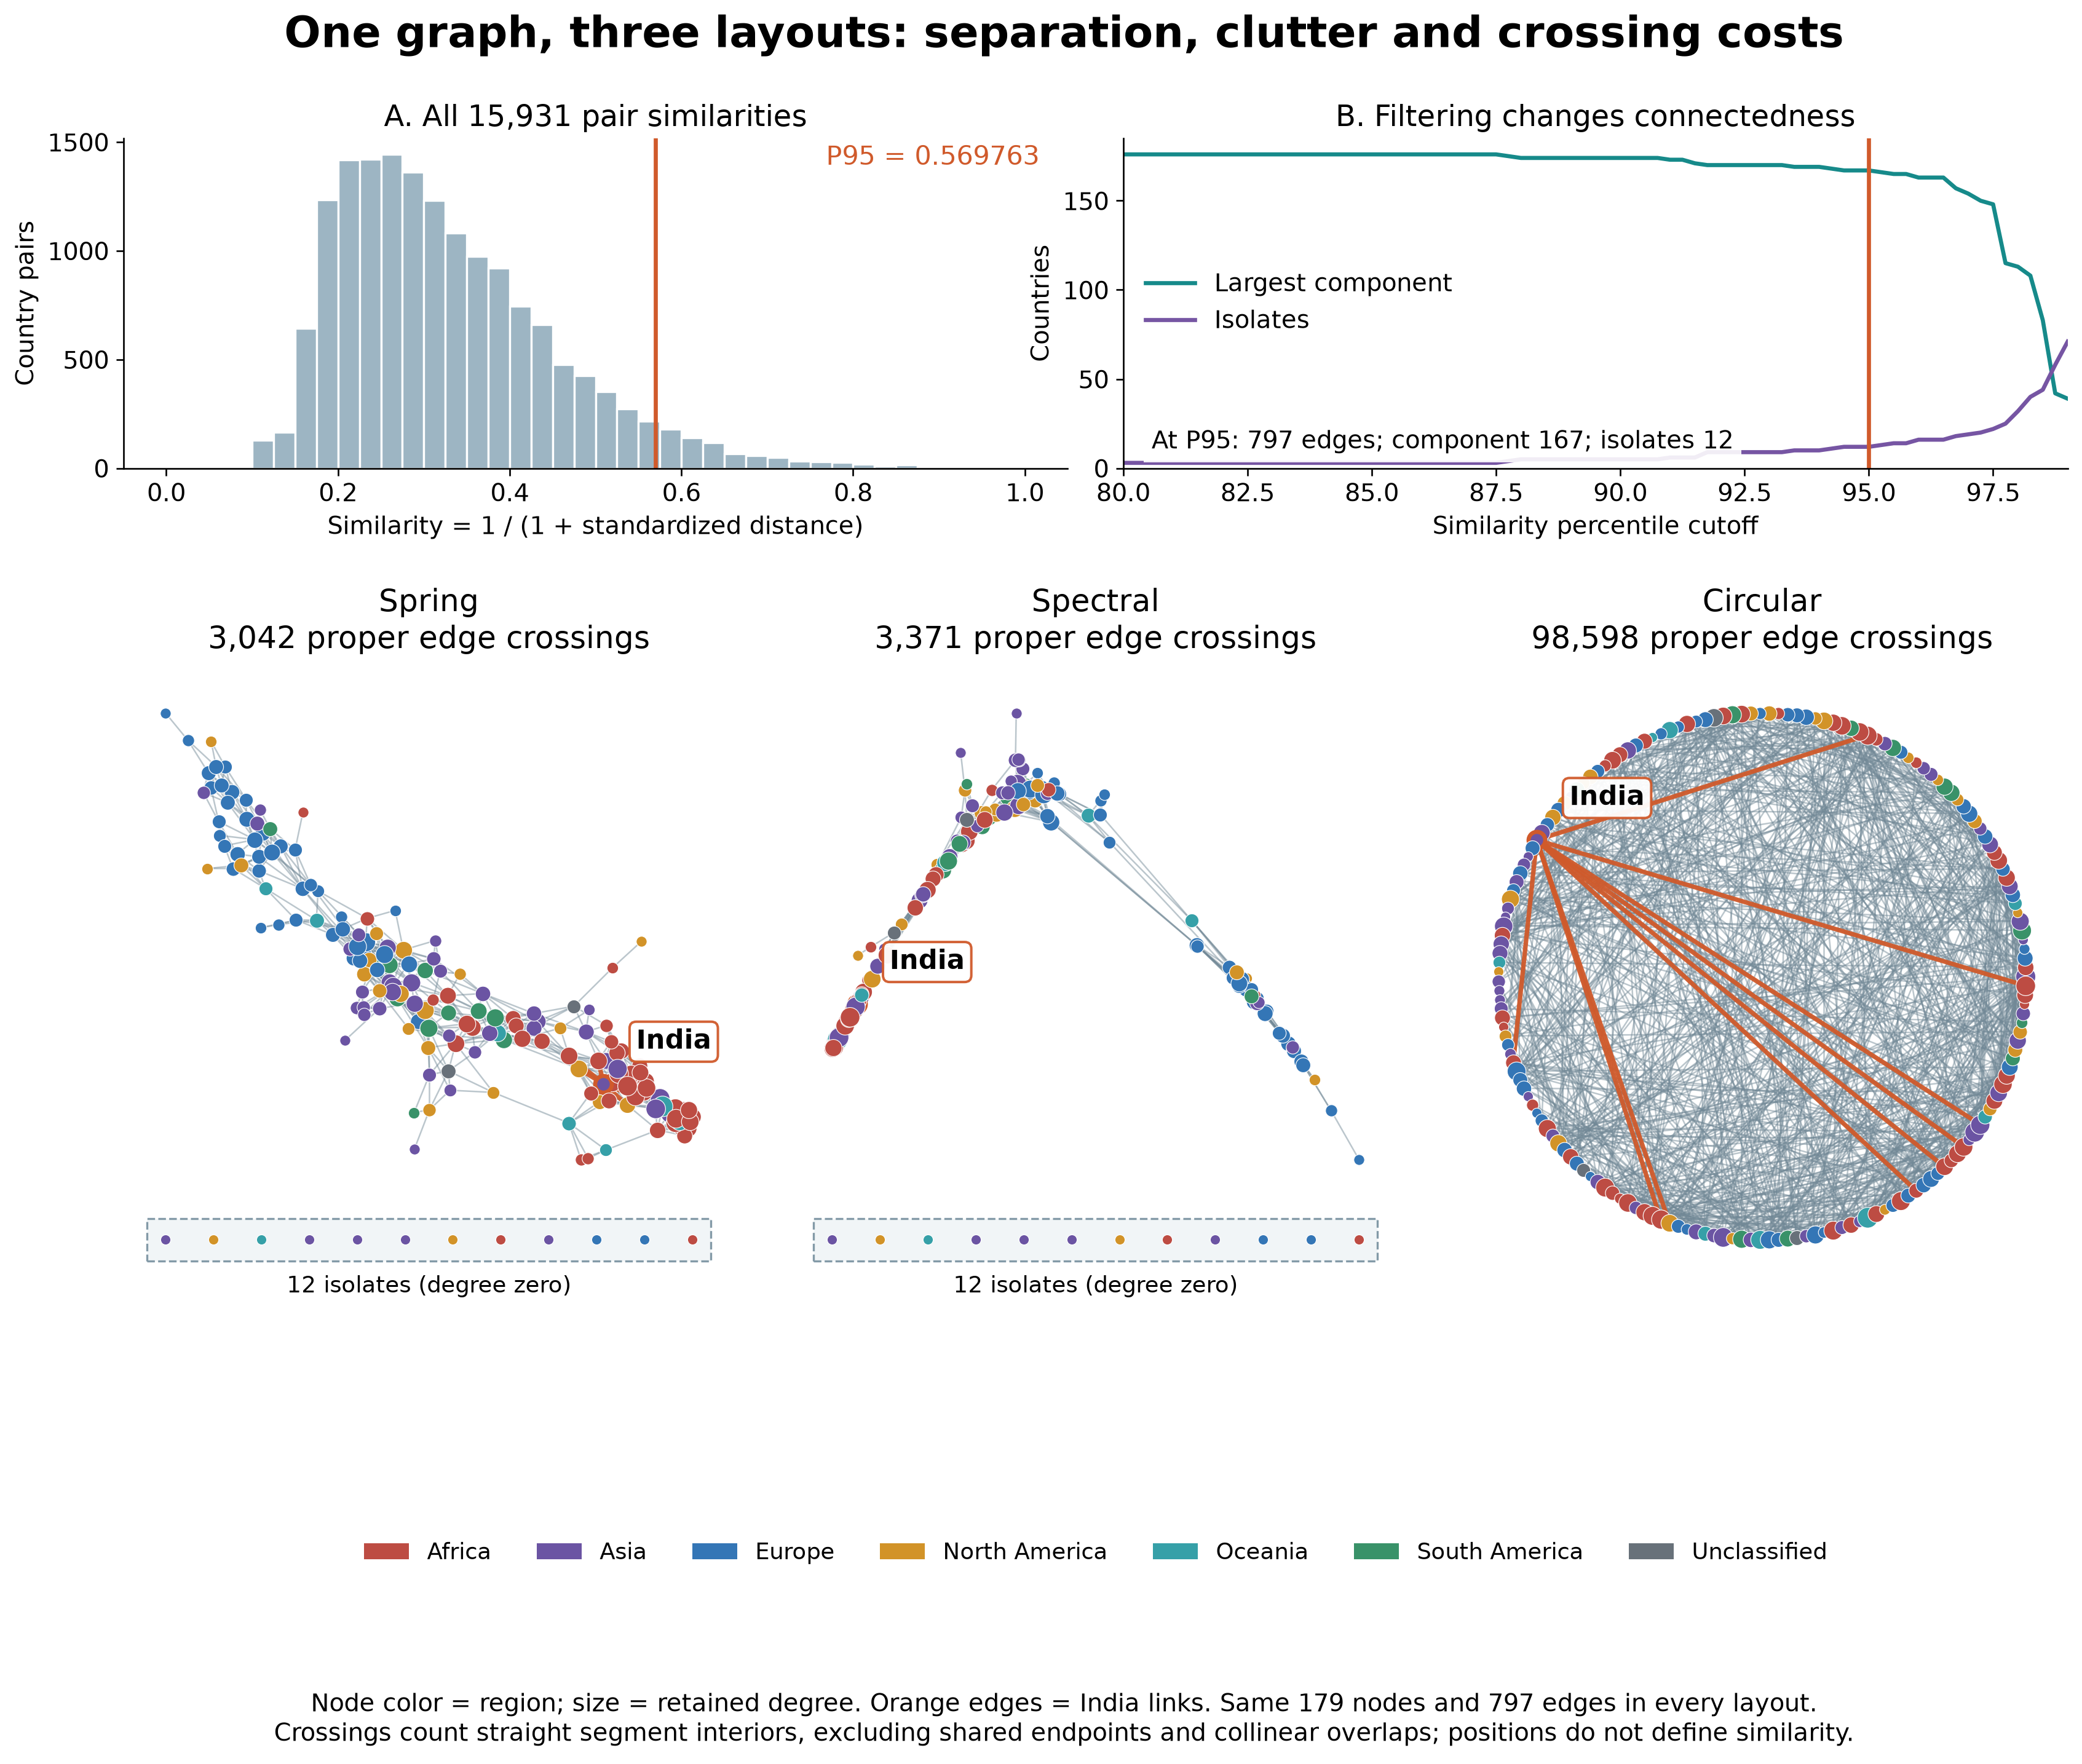
\includegraphics[width=\textwidth,height=0.63\textheight,keepaspectratio]{Fig1.png}

\caption{P95 keeps 797 edges and 12 isolates. Layouts preserve neighbors while changing separation and crossing costs; boxed rows deliberately place isolates. {\footnotesize \href{https://aithal007.github.io/DV_assignment2/web/network.html}{\textcolor{accent}{\underline{View live demonstration}}} \quad | \quad \href{https://aithal007.github.io/DV_assignment2/interactions.html\#network}{\textcolor{accent}{\underline{Full UI screenshot}}}}}\label{fig:1}

\end{figure*}

\noindent\textit{How to read the graph.} n=179 complete 2020 profiles. Top: pair scores and cutoff sensitivity. Bottom: region-colored, degree-sized nodes; orange edges highlight India.

\paragraph{Question.} How can a dense complete similarity network be filtered transparently before comparing layouts?



\paragraph{Visual encoding.} Cohort: 179 complete four-indicator profiles in 2020; no 2015 completeness is required. The histogram counts all unique country pairs. The second panel sweeps percentile cutoffs from P80 to P99 and counts countries in the largest connected component and countries with no retained edge. The vertical lines mark P95. The lower panels draw the same 797 retained edges with Spring, Spectral and Circular positions; India and its twelve links are highlighted.



\paragraph{Why this visualization.} The full similarity distribution makes the filtering decision visible instead of silently imposing nearest neighbors. Three layouts then test representation effects on one fixed threshold graph. A shared threshold treats every country pair by the same rule.



\paragraph{Interpretation.} The distribution defines the complete 15,931-pair universe. $P_{95}=0.569763$ retains 797 edges and all 179 countries, including 12 isolates. This is the team's sparse default; P90/P92.5/P97.5 retain 1,594/1,195/399 pairs and 5/9/22 isolates. The boxed bottom rows deliberately place degree-zero countries.

All layouts preserve India's twelve links. The Spectral horseshoe and Spring linear core show that the four indicators project mostly along one broad developmental direction in these layout projections. Spring separates the connected core with relatively short edges; Spectral compresses some neighborhoods and can overlap nodes; Circular preserves a uniform node order but creates 98,598 edge crossings, contrasting with 3,042 in Spring and 3,371 in Spectral. Region color and degree size expose composition and connectivity.

Metric and feature sensitivity analysis confirms that while perturbation with Gaussian noise (SD 0.02) yields high edge stability (mean Jaccard 0.922, range 0.905-0.941), omitting one indicator yields Jaccard overlaps of only 0.338 to 0.512: omitting mobile subscriptions gives Jaccard 0.338; fixed broadband 0.412; fixed landlines 0.485; and internet adoption 0.512. Alternative scaling yields overlaps of 0.801 (median/IQR) and 0.460 (ranks). Thus, P95 identifies a specific multi-indicator similarity cohort rather than an immutable country grouping.



\paragraph{Scope and reading note.} The upper 5\% is an analyst-selected starting view, not a significance cutoff or unique optimum. Isolates remain countries in the analysis. Standardization, features and threshold influence the edges; positions do not define neighbors.



\takeaway{Filtering makes the complete pair network readable, but also changes connectedness. P95 keeps 797 edges and 12 isolates; the three layouts preserve those relationships. Infer similarity from scores and edges, while treating layout proximity and isolated placement as display choices.

}

\noindent\textit{Analytical recommendation.} Compare exact neighbors across layouts before interpreting visual separation.

\subsection{Fig. 2: Different country paths to higher internet use}

\begin{figure*}[!tb]\centering

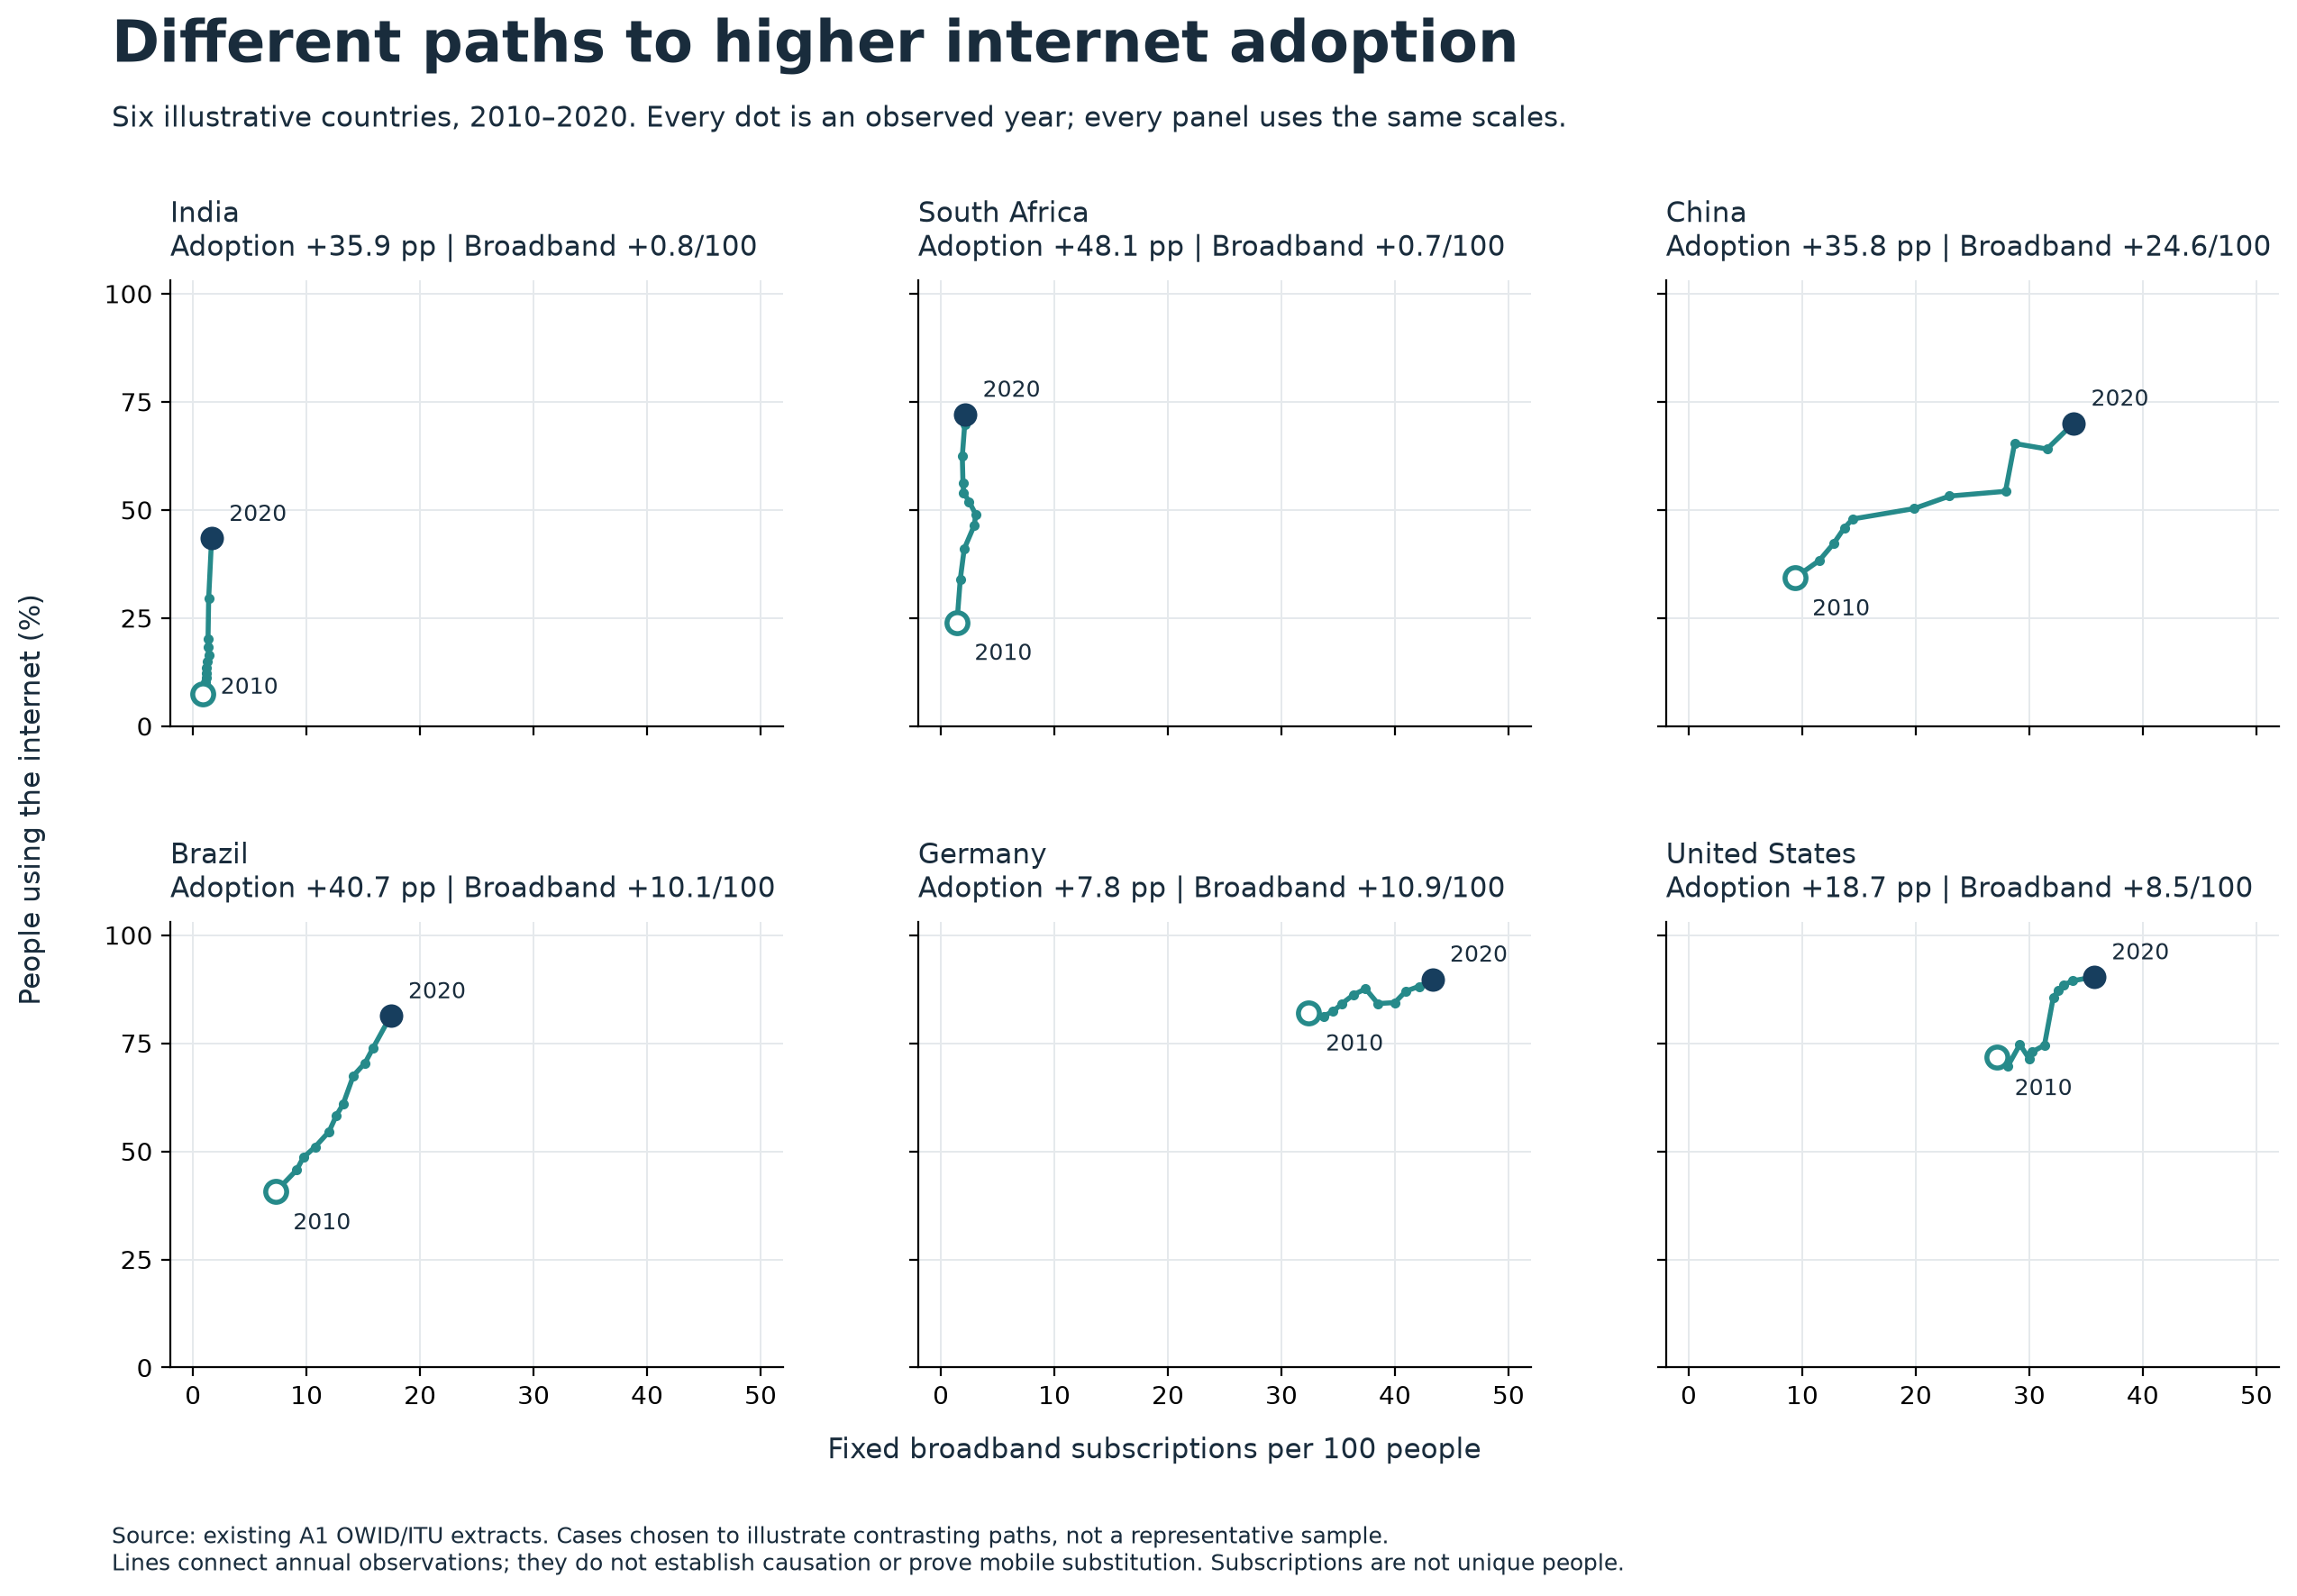
\includegraphics[width=0.99\textwidth,height=0.45\textheight,keepaspectratio]{Fig2.png}

\caption{Similar adoption gains accompany different annual infrastructure paths. {\footnotesize \href{https://aithal007.github.io/DV_assignment2/figures.html\#fig2}{\textcolor{accent}{\underline{View figure and interpretation online}}}}}\label{fig:2}

\end{figure*}

\noindent\textit{How to read the graph.} Six country panels retain annual 2010-2020 pairs on shared axes. Open/filled endpoints mark 2010/2020; intermediate dots preserve timing.

\paragraph{Question.} Can internet use rise without a similar rise in fixed broadband?



\paragraph{Visual encoding.} Each panel follows one country from 2010 to 2020. Open dots mark 2010 and dark dots mark 2020. Small dots show the intervening years. All panels use the same axes.



\paragraph{Why this visualization.} The network compares countries in one year. Small multiples add the history it leaves out. Each country gets its own panel, so its annual path can be followed without crossing five other paths. Shared axes make the size and direction of the changes comparable across countries.



\paragraph{Interpretation.} The six panels do not follow one shared adoption-broadband path. South Africa gains 48.1 percentage points in internet use with only 0.7 additional fixed-broadband subscriptions per 100 people, whereas China gains 35.8 points with 24.6 additional subscriptions. India similarly gains 35.9 points with a broadband increase of 0.8. The vertical separation of their start/end markers and different horizontal displacements are the visible evidence.

This answers the history part of the main question: an endpoint or even a similar adoption gain cannot identify the associated infrastructure trajectory. Germany's smaller adoption gain also begins from an already high 82\% level, so raw gains need starting-level context. These six stated examples illustrate heterogeneity; they do not establish whether mobile access, investment or another mechanism caused it.



\paragraph{Scope and reading note.} These six examples illustrate different paths. They do not represent every country or prove what caused the change.



\takeaway{Similar adoption progress can accompany different infrastructure histories. The contrasting country paths show that a 2020 endpoint cannot establish how a country reached it; annual paired observations are needed to distinguish those histories.

}

\noindent\textit{Analytical recommendation.} Use annual paths to distinguish countries with similar endpoint gains.

\subsection{Fig. 3: Community links and degree-ordered pair detail}

\begin{figure*}[!tb]\centering

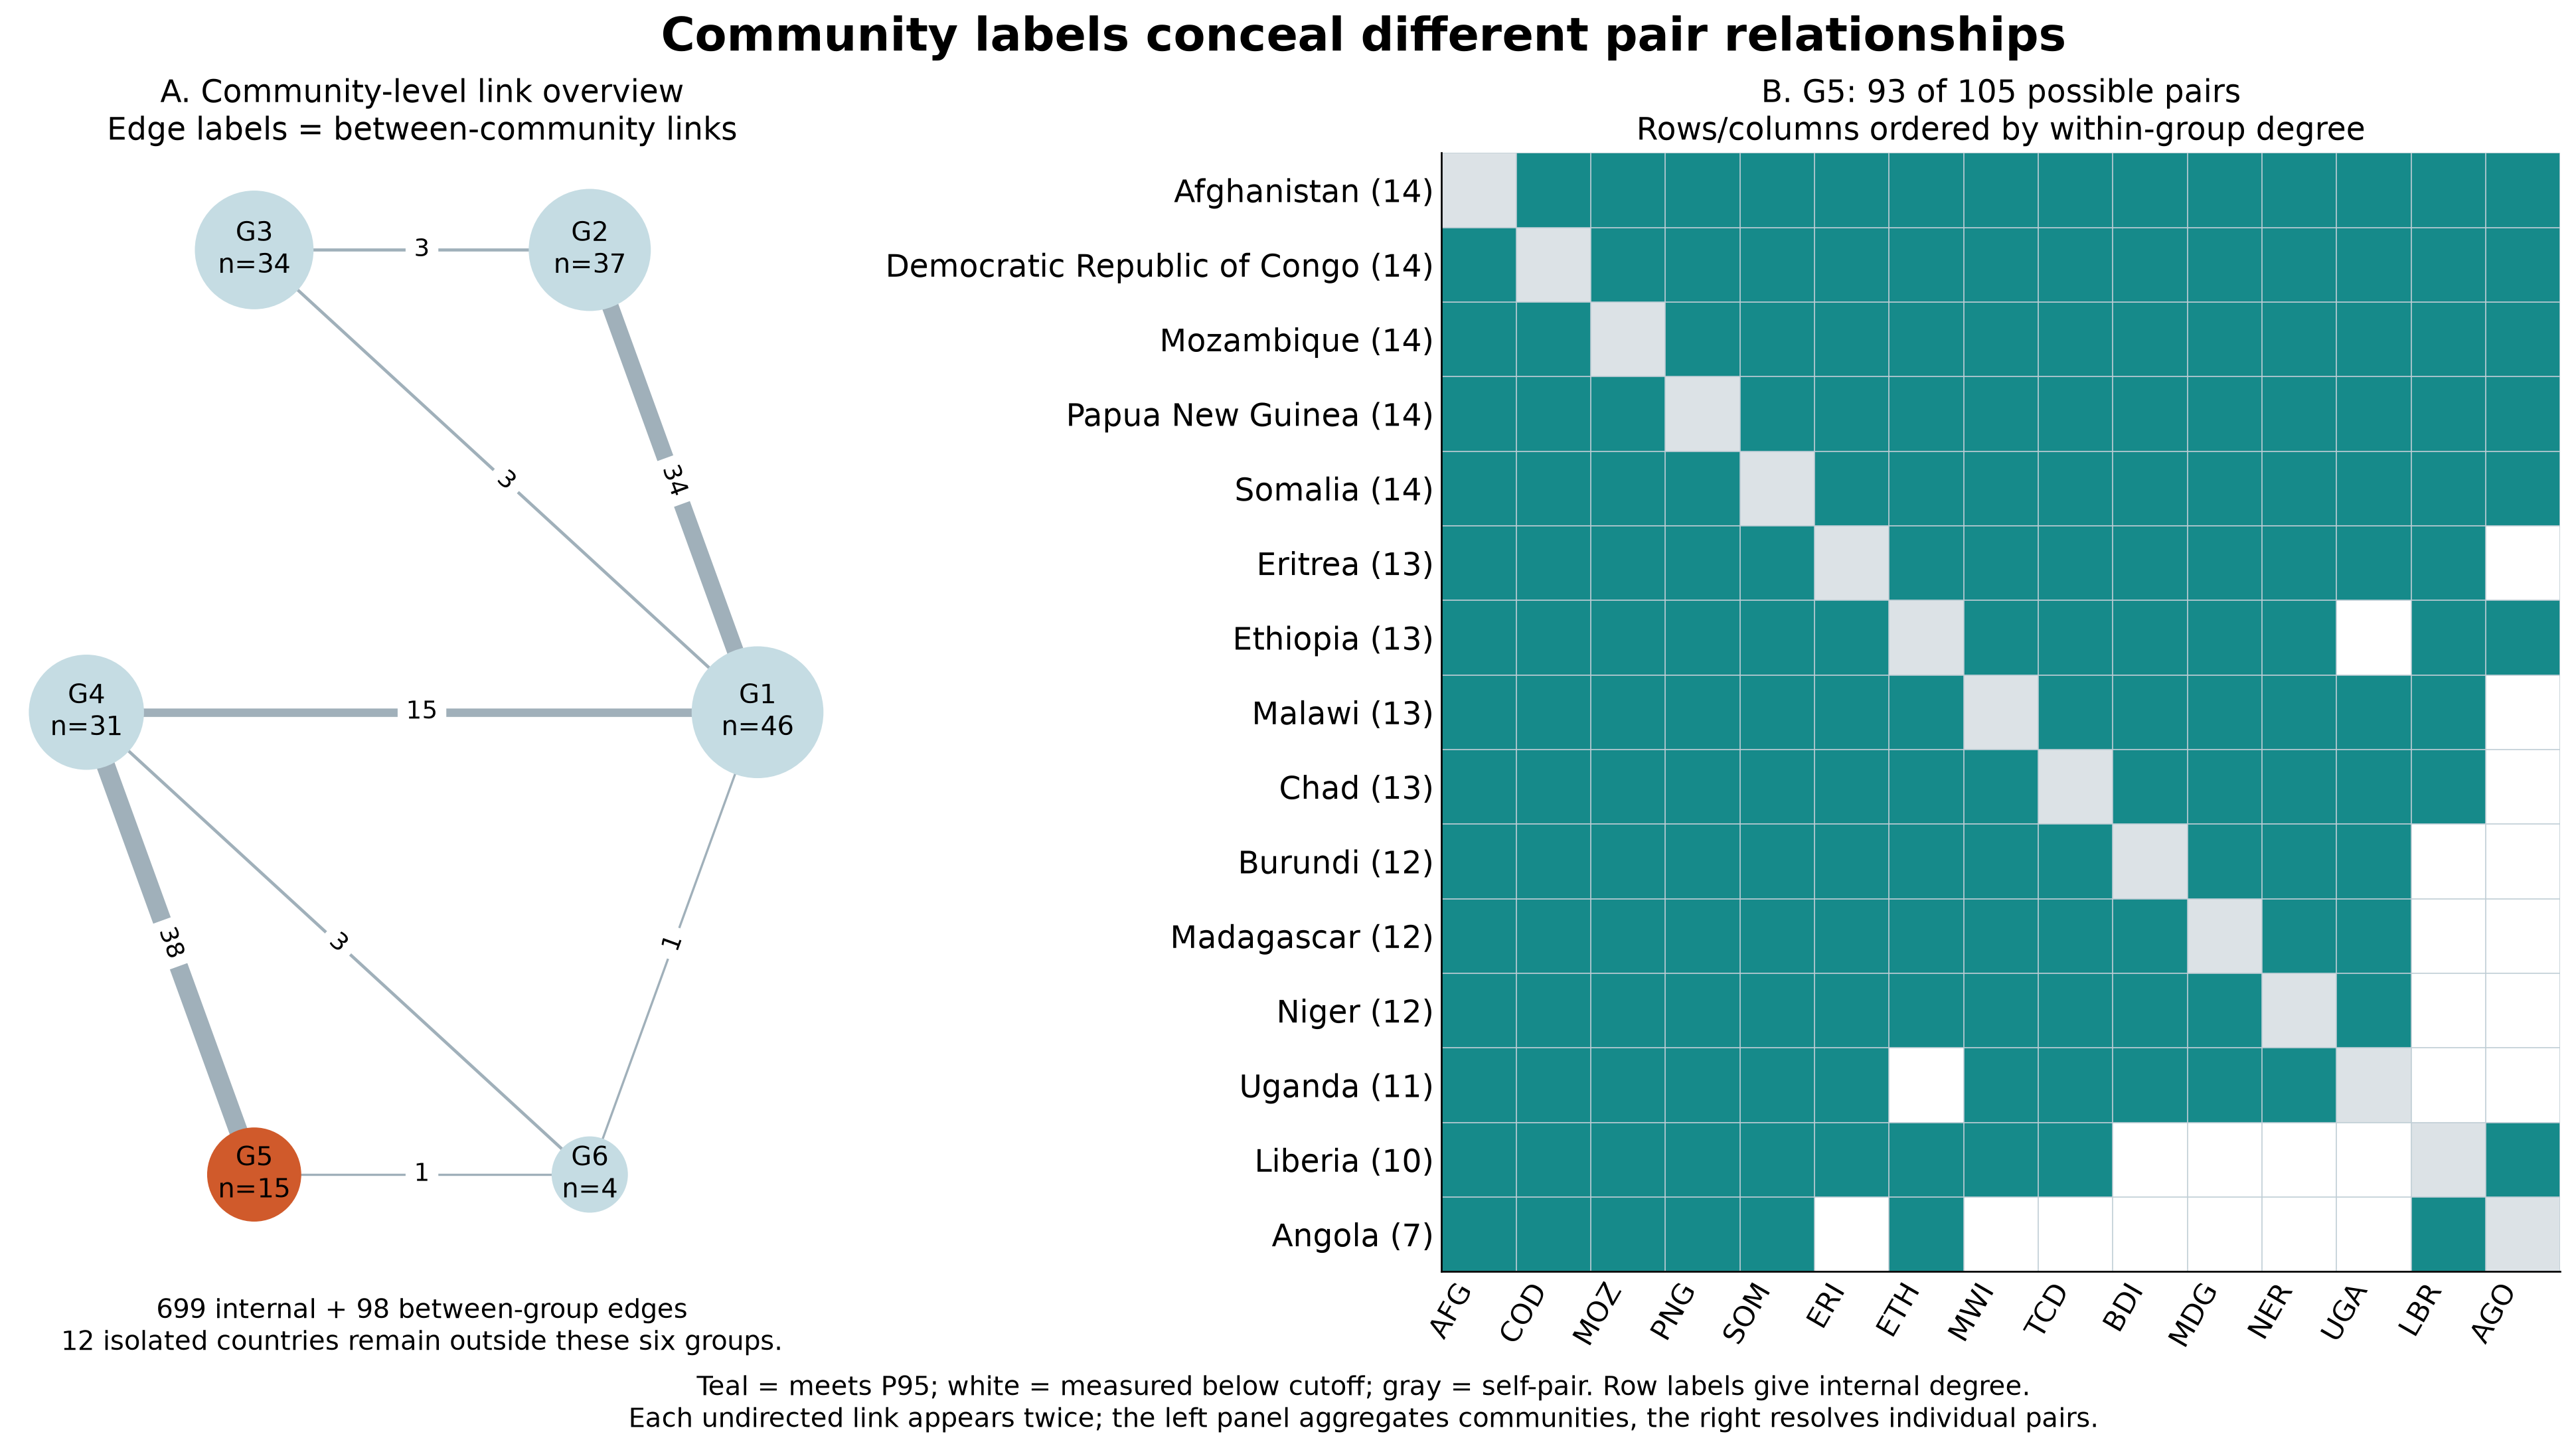
\includegraphics[width=0.99\textwidth,height=0.55\textheight,keepaspectratio]{Fig3.png}

\caption{A shared community label conceals unequal internal degrees and measured gaps. {\footnotesize \href{https://aithal007.github.io/DV_assignment2/figures.html\#fig3}{\textcolor{accent}{\underline{View figure and interpretation online}}}}}\label{fig:3}

\end{figure*}

\noindent\textit{How to read the graph.} Left: aggregate community nodes and between-group edge counts. Right: degree-ordered individual pairs; teal meets P95, white does not, gray excludes self-pairs.

\paragraph{Question.} Which individual relationships are hidden by the grouped threshold graph?



\paragraph{Visual encoding.} Left: six aggregate community nodes, sized by country count, with between-community edge counts. Right: the selected 15-country adjacency matrix, ordered by descending internal degree. Teal means above cutoff, white below, gray self-pair.



\paragraph{Why this visualization.} Matrix cells make exact retained pairs and gaps checkable without relying on crowded lines. The detail group is selected reproducibly as the smallest group with at least five countries that is not a clique. Isolates are explicitly reported rather than silently dropped.



\paragraph{Interpretation.} The left graph aggregates six communities, making their 98 between-group links readable; the 699 internal links remain inside the groups. The right matrix resolves the selected 15-country group, with 93 of 105 possible links. Rows and columns are arranged by descending internal degree, so dense members and gaps are immediately visible without decoding miniature overview matrices.

Afghanistan has 14 internal neighbors and Angola seven: a shared group label conceals different pair relationships. White cells are measured scores below P95; the diagonal is excluded. This node-link/matrix hybrid is inspired by NodeTrix \cite{ref8}, while community nodes in the overview are aggregates. The exact matrix supplies the individual evidence that the grouped picture omits.



\paragraph{Scope and reading note.} Groups are weighted greedy-modularity summaries of the threshold graph, not natural country types. A white cell does not mean no measured similarity: every distinct pair has a score, but this pair falls below the current cutoff.



\takeaway{A community label hides unequal relationships among its members. The enlarged matrix contains 93 of 105 possible links, with uneven row degrees and real gaps. Inspect those pairs before treating a network community as one uniform telecom profile.

}

\noindent\textit{Analytical recommendation.} Inspect individual pairs before generalizing from a community label.

\section{Profiles, changes and hierarchies}

We connect paired changes and endpoint profiles, directly test almost equal adoption, then compare associations and user-count hierarchies.



\subsection{Fig. 4: Similar internet gains, different infrastructure changes}

\begin{figure*}[!tb]\centering

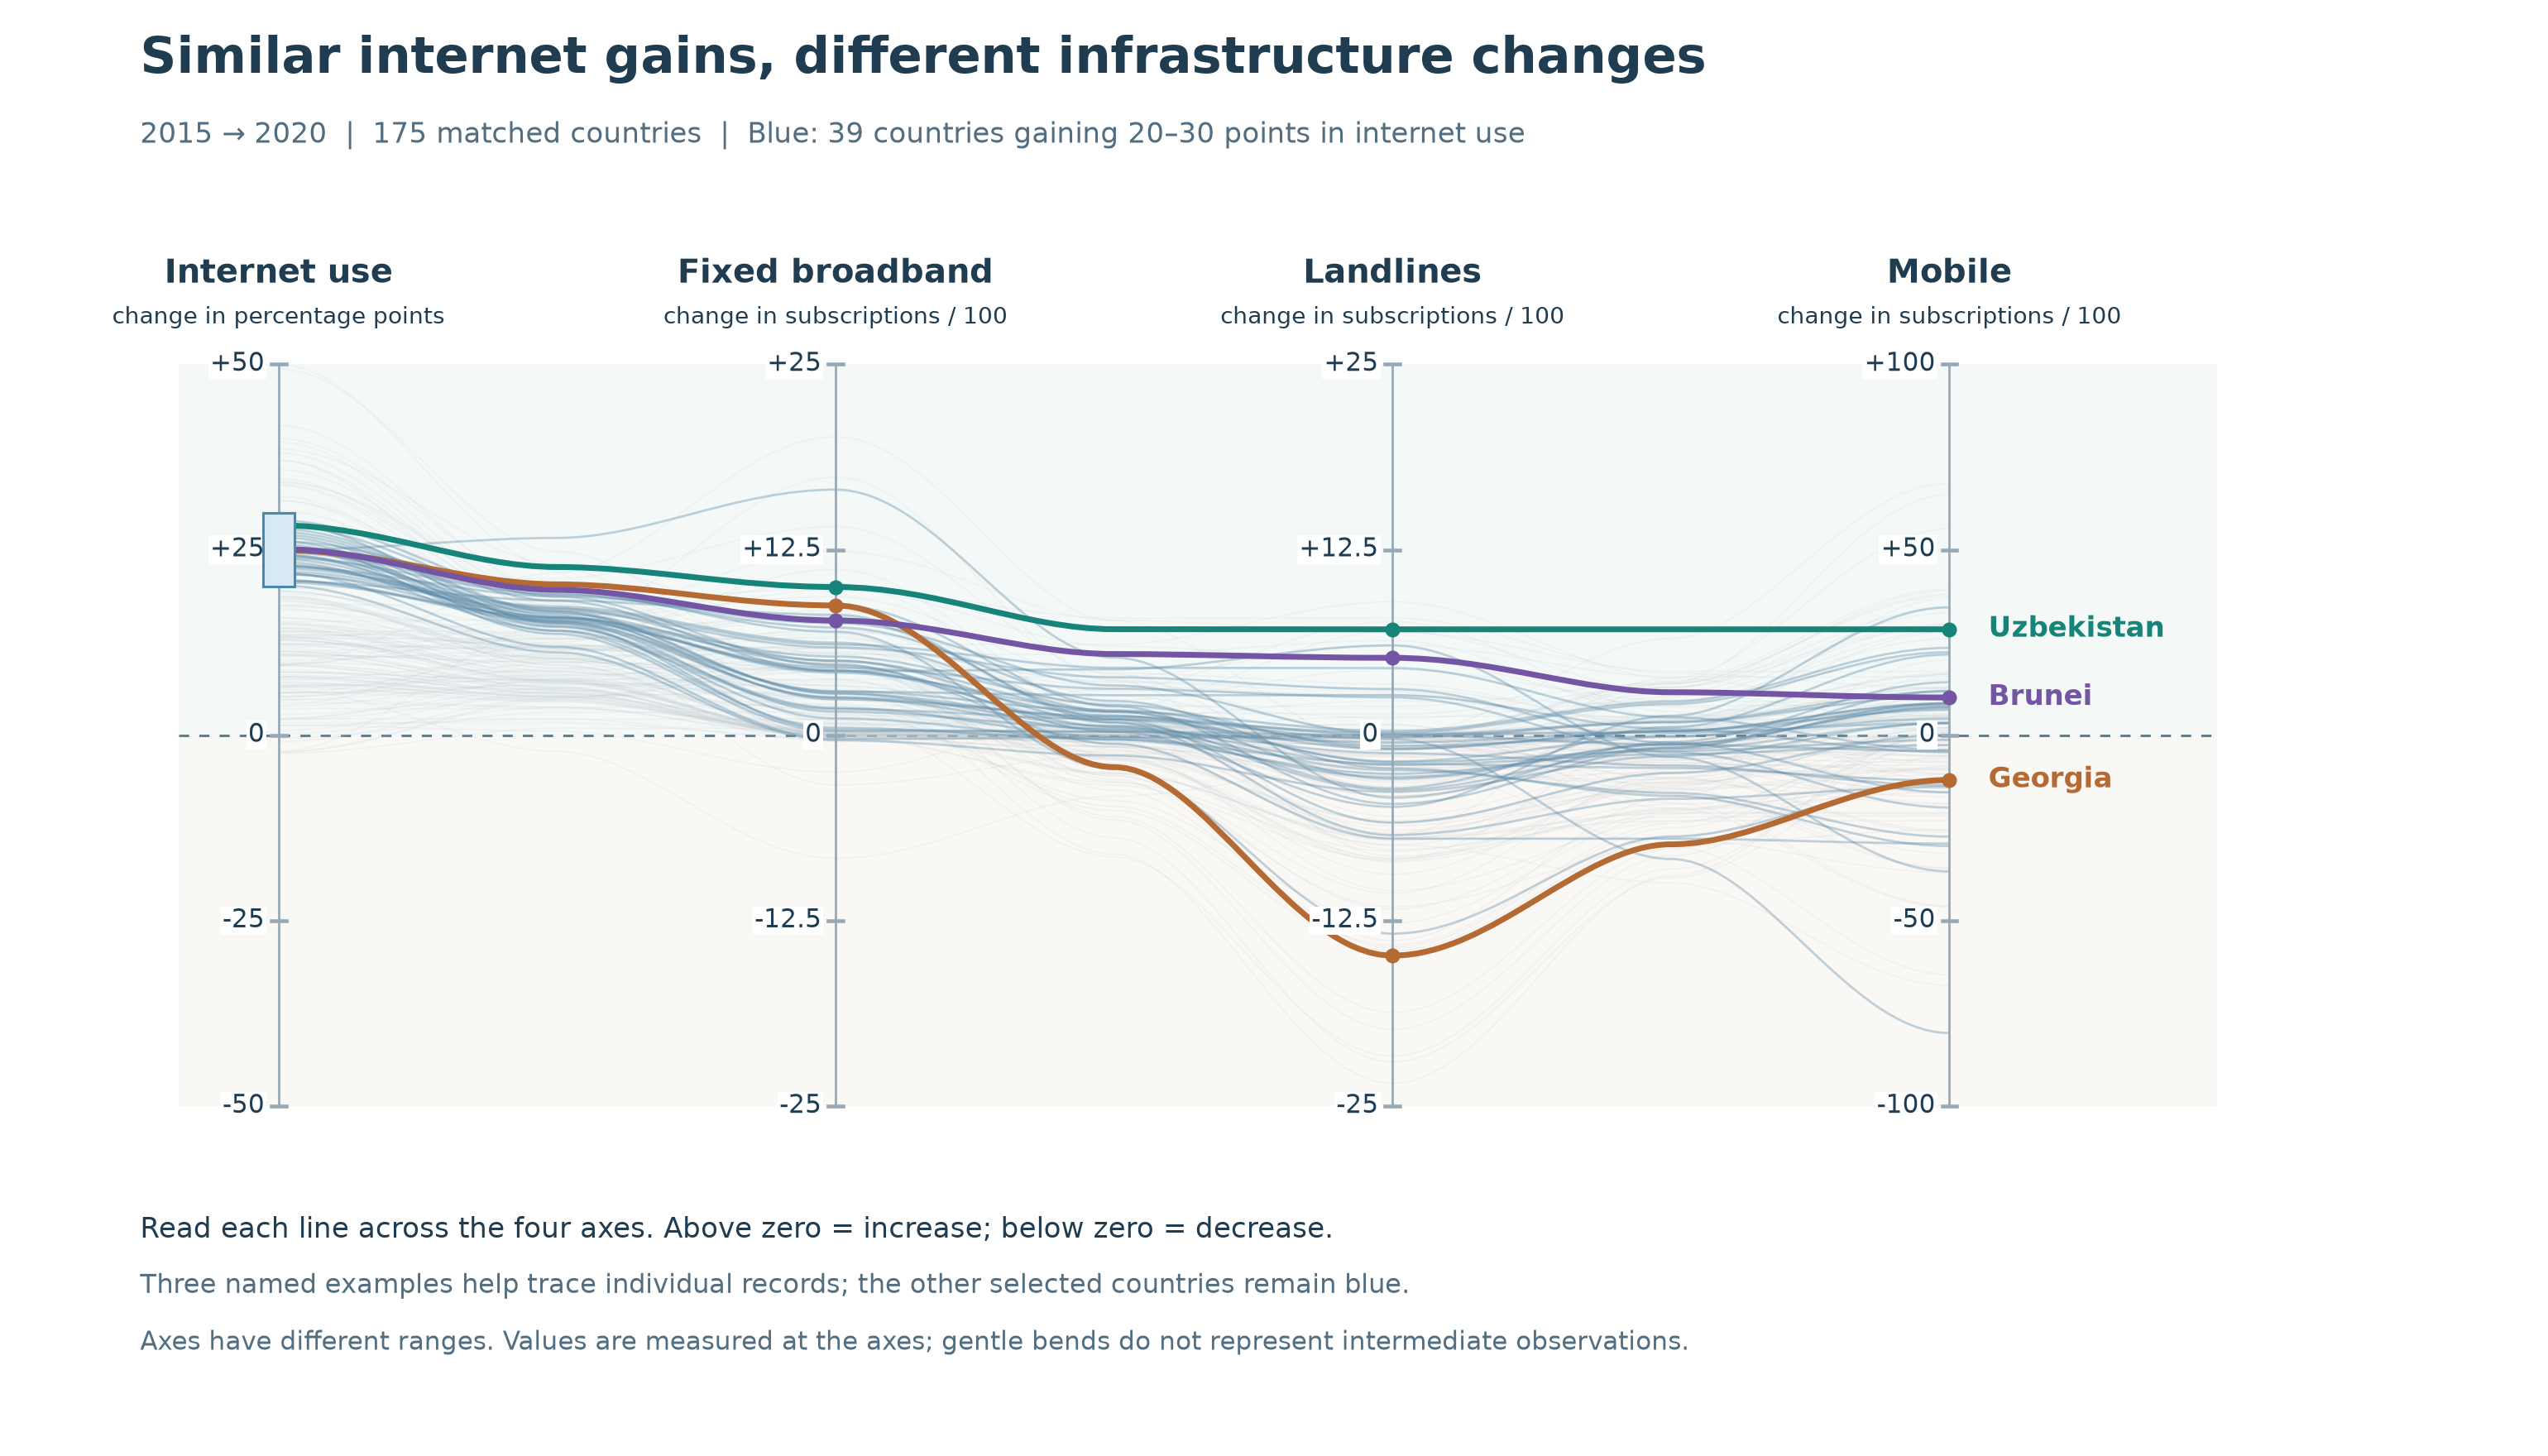
\includegraphics[width=\textwidth,height=0.49\textheight,keepaspectratio]{Fig4.png}

\caption{One adoption-gain band contains opposing landline and mobile changes. {\footnotesize \href{https://aithal007.github.io/DV_assignment2/output/pcp_changes/index.html}{\textcolor{accent}{\underline{View live demonstration}}} \quad | \quad \href{https://aithal007.github.io/DV_assignment2/interactions.html\#changes}{\textcolor{accent}{\underline{Full UI screenshot}}}}}\label{fig:4}

\end{figure*}

\noindent\textit{How to read the graph.} n=175 matched 2015/2020 countries. Axes show within-country changes; zero is aligned. The brush highlights 20-30-point adoption gains; three examples are named.

\paragraph{Question.} Do countries with similar gains in internet use also have similar changes in their telecom indicators?



\paragraph{Visual encoding.} Cohort: the same 175 countries complete in both 2015 and 2020; four other 2020-complete countries lack complete 2015 profiles. Each line connects one country's four changes from 2015 to 2020. At every axis, change is calculated as the 2020 value minus its 2015 value. Internet use changes in percentage points; the other axes show changes in subscriptions per 100 people. All 175 matched countries remain visible. Blue highlights the 39 countries that gained 20-30 percentage points in internet use; gray retains the other 136. Three selected examples are named and colored separately. The dashed horizontal line aligns zero on all four axes: above it means an increase and below it a decrease. Each axis has its own stated range.



\paragraph{Why this visualization.} The annual paths in Fig.~\ref{fig:2} compare internet use and broadband for six examples. This parallel-coordinate view connects all four changes for the full matched sample, so one country can be followed across several measures. Brushing a common range of internet gains asks what else changed among countries making broadly similar progress. Thin background lines retain the full sample, while three named records make the selected pattern easier to trace. The browser supports brushing, axis reordering, hover values and a straight-versus-gently-bundled comparison.



\paragraph{Interpretation.} The gain brush selects 39 of the same 175 matched countries. Within this 20-30-point adoption band, broadband changes span about -0.3 to +16.6, landlines -14.8 to +7.1 and mobile -80.2 to +34.5 subscriptions per 100. One adoption-gain interval therefore conceals several infrastructure transitions.

Georgia and Brunei both gain about 25 adoption points and eight broadband subscriptions, yet their landline/mobile changes are -14.8/-12.0 versus +5.2/+10.2. Uzbekistan gains 28.3 adoption points, 10.0 broadband, 7.1 landline and 28.6 mobile subscriptions. Its positive movement on all four axes contrasts with the other named cases. Values are read precisely at vertical axis intercepts; bundled curves are visual tracing aids that preserve categorical cluster cohesion \cite{ref10}.



\paragraph{Scope and reading note.} The selected gain range is descriptive. Different axis ranges preserve a shared zero position, but equal heights or slopes do not mean equal changes in the four units.



\takeaway{Similar internet-use gains conceal different combinations of infrastructure change. Even the selected 20-30-point gain group contains opposing landline and mobile movements. Follow each country across all four change axes before assigning one explanation to its progress.

}

\noindent\textit{Analytical recommendation.} Trace all four country changes before assigning one transition story.

\subsection{Fig. 5: Gentle bundles reveal different country profiles}

\begin{figure*}[!tb]\centering

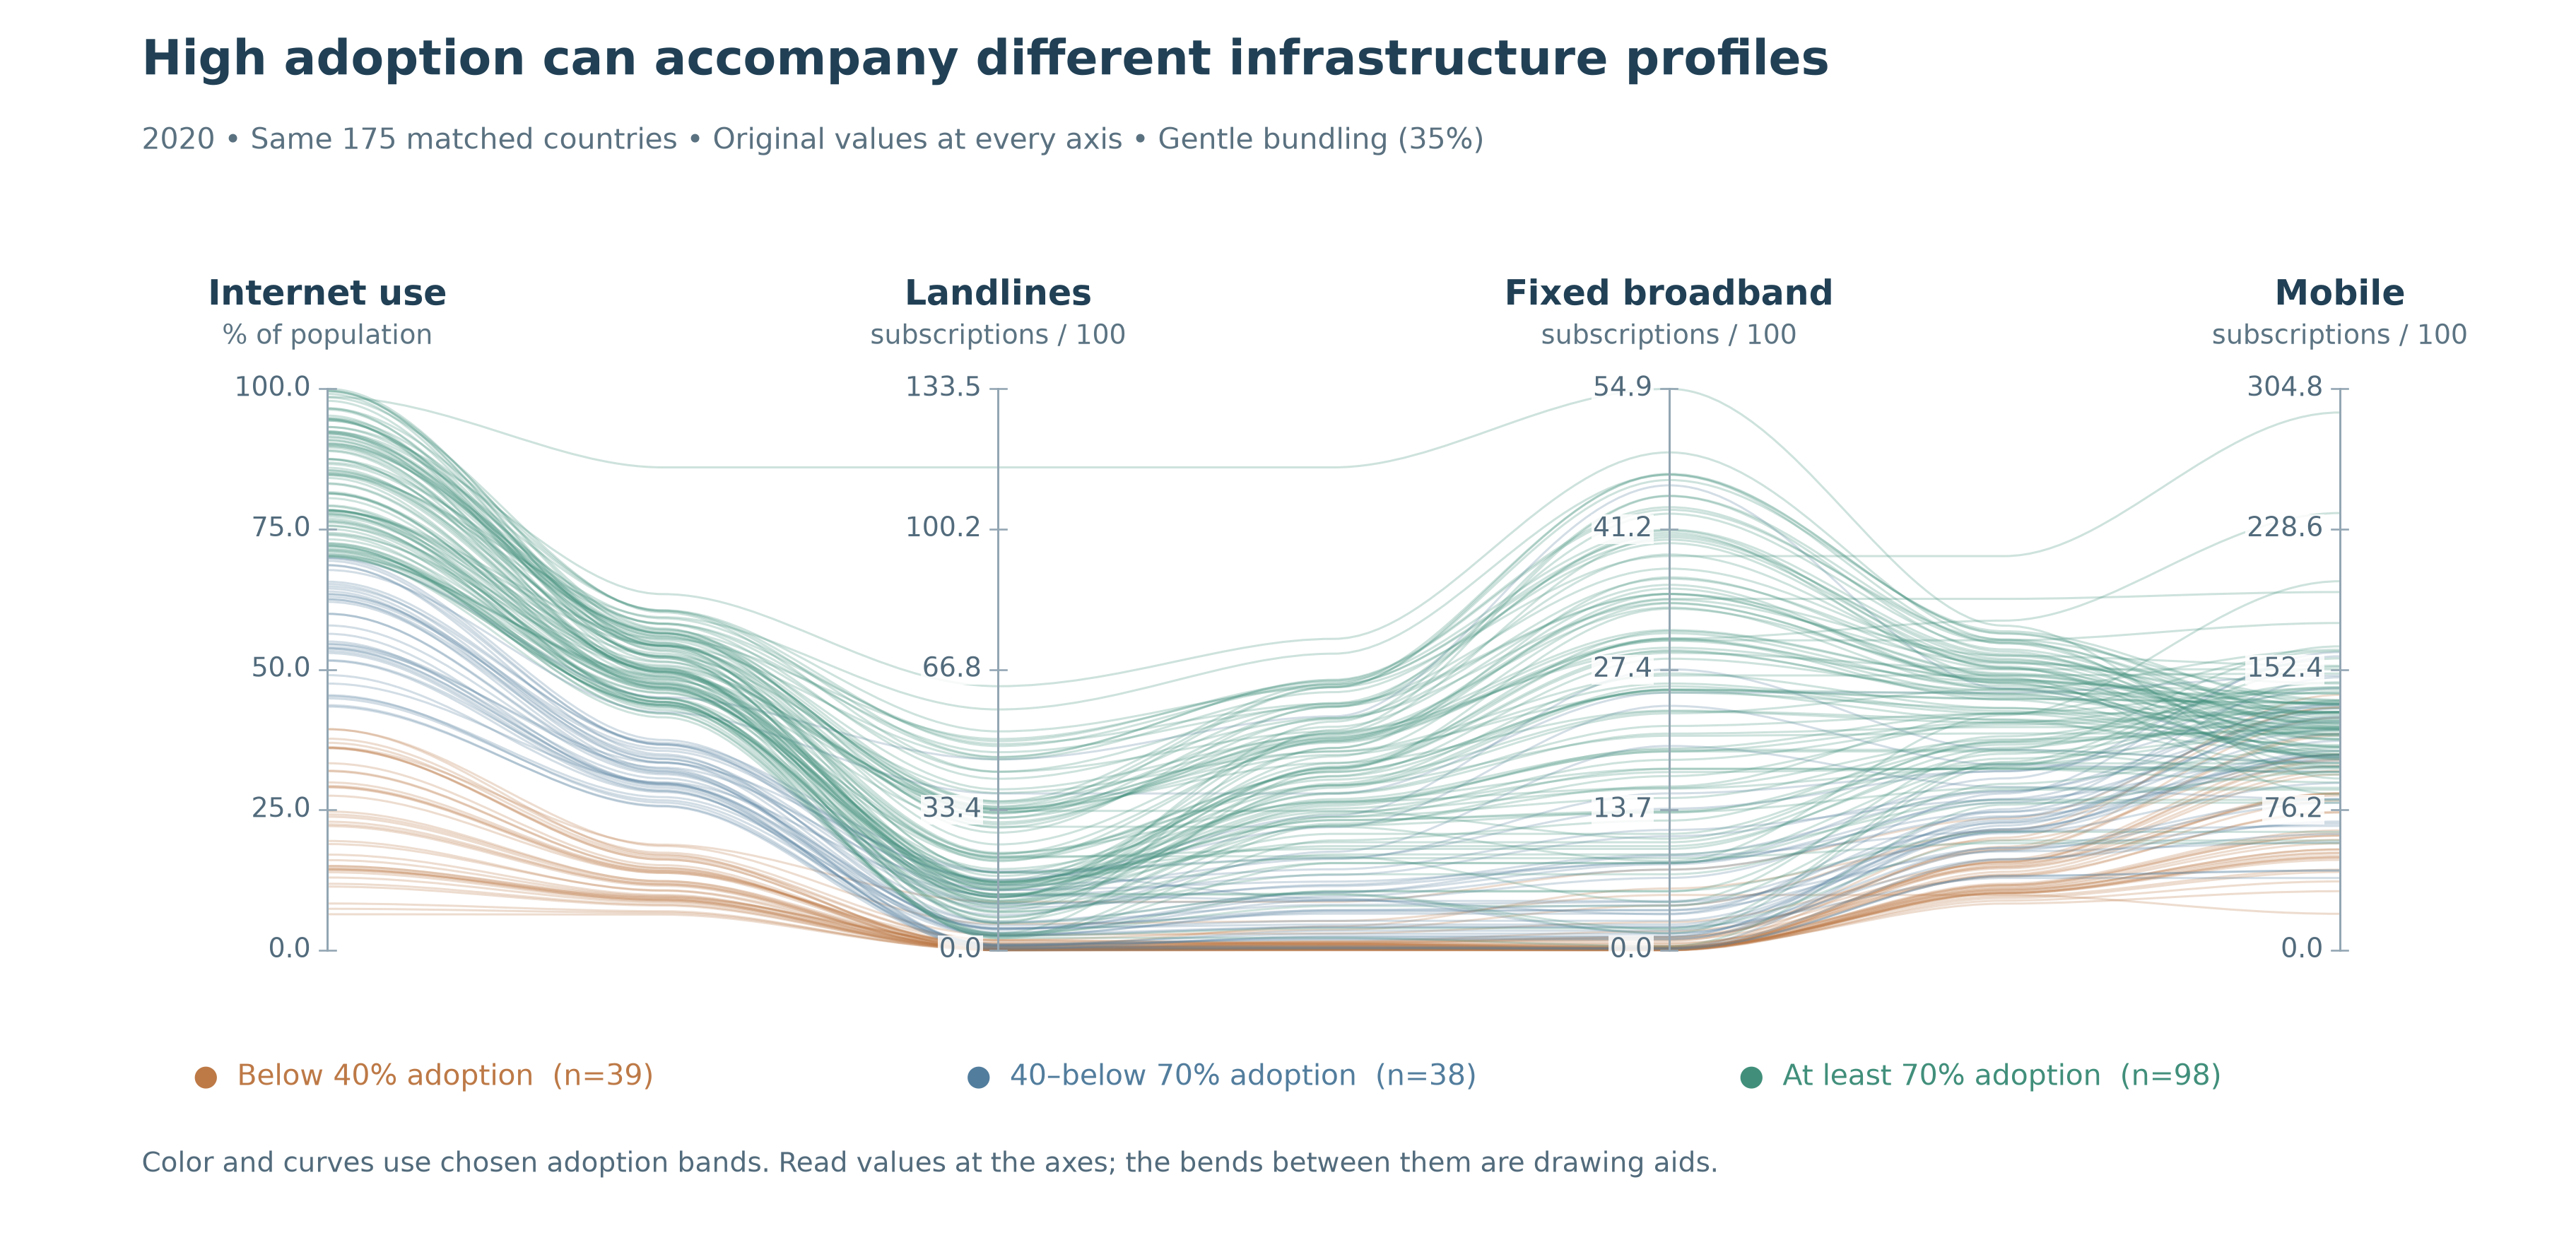
\includegraphics[width=\textwidth,height=0.49\textheight,keepaspectratio]{Fig5.png}

\caption{High-adoption countries retain different four-indicator profiles. {\footnotesize \href{https://aithal007.github.io/DV_assignment2/web/index.html}{\textcolor{accent}{\underline{View live demonstration}}} \quad | \quad \href{https://aithal007.github.io/DV_assignment2/interactions.html\#pcp}{\textcolor{accent}{\underline{Full UI screenshot}}}}}\label{fig:5}

\end{figure*}

\noindent\textit{How to read the graph.} n=175 matched countries, shown in 2020. Adoption-band colors/bundles organize four measured axes. Read at intercepts; the browser retains brushes and ordering controls.

\paragraph{Question.} Do countries with high internet use share the same infrastructure profile?



\paragraph{Visual encoding.} Cohort: the same 175 countries complete in both 2015 and 2020; four other 2020-complete countries lack complete 2015 profiles. Each curve is one of the same 175 countries in 2020. The four vertical axes retain their original units and full matched-country ranges. Orange means below 40\% internet use, blue means 40-below-70\%, and green means at least 70\%. Within each chosen band, curves are bundled using category-based centroid attractor splines: cubic B-spline paths attract lines toward their band's inter-axis centroid at 35\% bundling strength, reducing visual clutter between axes while strictly preserving exact intercept positions on each vertical axis. These bands are chosen comparison groups, not discovered country types.



\paragraph{Why this visualization.} Parallel coordinates keep four measurements connected for each country. Thin curves and three consistent colors make the full set easier to follow without replacing records with filled ribbons. Fig.~\ref{fig:4} compares five-year changes; this figure compares the country profiles at the 2020 endpoint. The two PCPs therefore ask different questions using the same matched countries. The browser lets the reader compare straight and bundled paths, brush ranges, reorder axes and inspect country values.



\paragraph{Interpretation.} The high-adoption curves fan out strongly on fixed broadband. Kuwait has about 99.1\% internet use with 1.7 broadband subscriptions per 100 people; Kyrgyzstan has 72.0\% with 4.3. Mobile values also overlap across the three adoption bands instead of separating them cleanly. These are visible exceptions to the idea that one headline adoption category has one infrastructure profile.

Read values where each curve meets an axis. Gentle bundling uses the declared adoption bands to help trace records \cite{ref10}, while the joins between axes are drawing aids. This plot addresses endpoint composition; the preceding change plot addresses transition. Together they distinguish a similar present state from a similar history. The data do not measure all alternative access technologies or identify a causal route to connectivity.



\paragraph{Scope and reading note.} Adoption bands are descriptive choices. Only axis intersections are observations; bundling does not establish causes.



\takeaway{High adoption describes several infrastructure profiles rather than one common model. Overlapping mobile values and widely differing broadband values within the same adoption band show why the headline rate must be read alongside the other indicators.

}

\noindent\textit{Analytical recommendation.} Read the full profile before treating an adoption band as an infrastructure model.

\subsection{Fig. 6: Similar adoption can hide different infrastructure}

\begin{figure*}[!tb]\centering

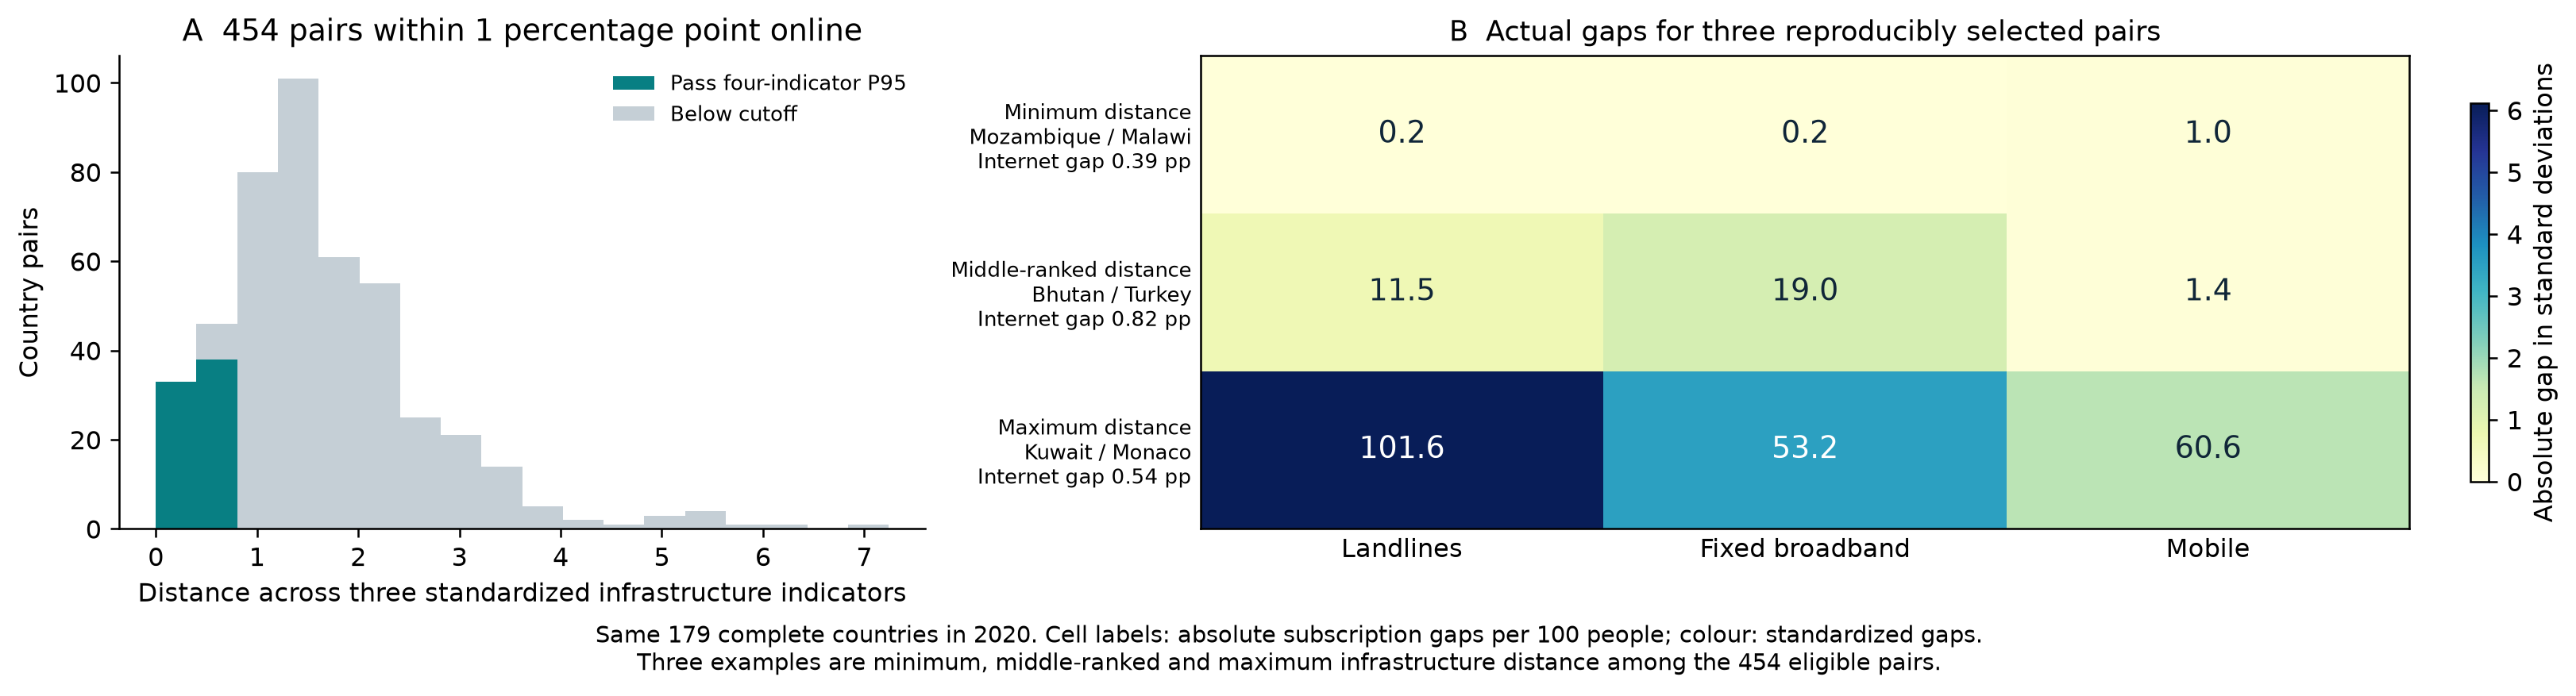
\includegraphics[width=\textwidth,height=0.28\textheight,keepaspectratio]{Fig6.png}

\caption{Nearly equal adoption, differing infrastructure. Histogram distance uses three infrastructure indicators; color tests the full four-indicator P95 rule. {\footnotesize \href{https://aithal007.github.io/DV_assignment2/figures.html\#fig6}{\textcolor{accent}{\underline{View figure and interpretation online}}}}}\label{fig:6}

\end{figure*}

\noindent\textit{How to read the graph.} n=179 complete 2020 profiles. Histogram distance uses three infrastructure indicators; pass/fail color uses four-indicator P95. Example cells label raw subscription gaps.

\paragraph{Question.} How much can infrastructure differ when internet-use rates almost match?



\paragraph{Visual encoding.} Cohort: 179 complete four-indicator profiles in 2020; no 2015 completeness is required. Panel A counts pairs within one percentage point in internet use. Panel B shows three pairs selected by minimum, middle-ranked and maximum infrastructure distance. Labels give absolute subscription gaps per 100 people; colour gives standardized gaps.



\paragraph{Why this visualization.} This links an almost equal headline rate to the infrastructure detail it conceals. The histogram retains all eligible pairs, while the examples make the gaps tangible.



\paragraph{Interpretation.} Among 454 country pairs whose adoption rates differ by at most 1.0 percentage point, only 71 (15.6\%) meet the full-profile P95 similarity cutoff. Because the P95 threshold retains exactly 5.0\% of all 15,931 country pairs by construction, this 15.6\% passing rate represents a 3.1x enrichment over the random baseline. While adoption proximity makes profile similarity more likely, 84.4\% of near-equal-adoption pairs still diverge in telecom infrastructure.

The histogram's horizontal axis measures standardized Euclidean distance across landline, broadband, and mobile subscriptions, while bar color indicates full four-indicator P95 compliance. Bhutan/Turkey differ by 0.82 adoption points but 19.0 broadband subscriptions per 100; Kuwait/Monaco show much larger infrastructure gaps despite a 0.54-point adoption gap. Headline adoption cannot substitute for full-profile evaluation.



\paragraph{Scope and reading note.} Pairs share countries and are not independent observations. Standardized distances depend on the chosen features; the examples are illustrative, not representative samples.



\takeaway{Almost equal adoption rates can conceal substantially different infrastructure. Only 71 of 454 eligible pairs meet the full-profile cutoff. The headline percentage therefore cannot substitute for a country profile, even when two values nearly match.

}

\noindent\textit{Analytical recommendation.} Compare the full profile even when headline adoption rates nearly match.

\subsection{Fig. 7: Four telecom measures: associations and exceptions}

\begin{figure*}[!tb]\centering

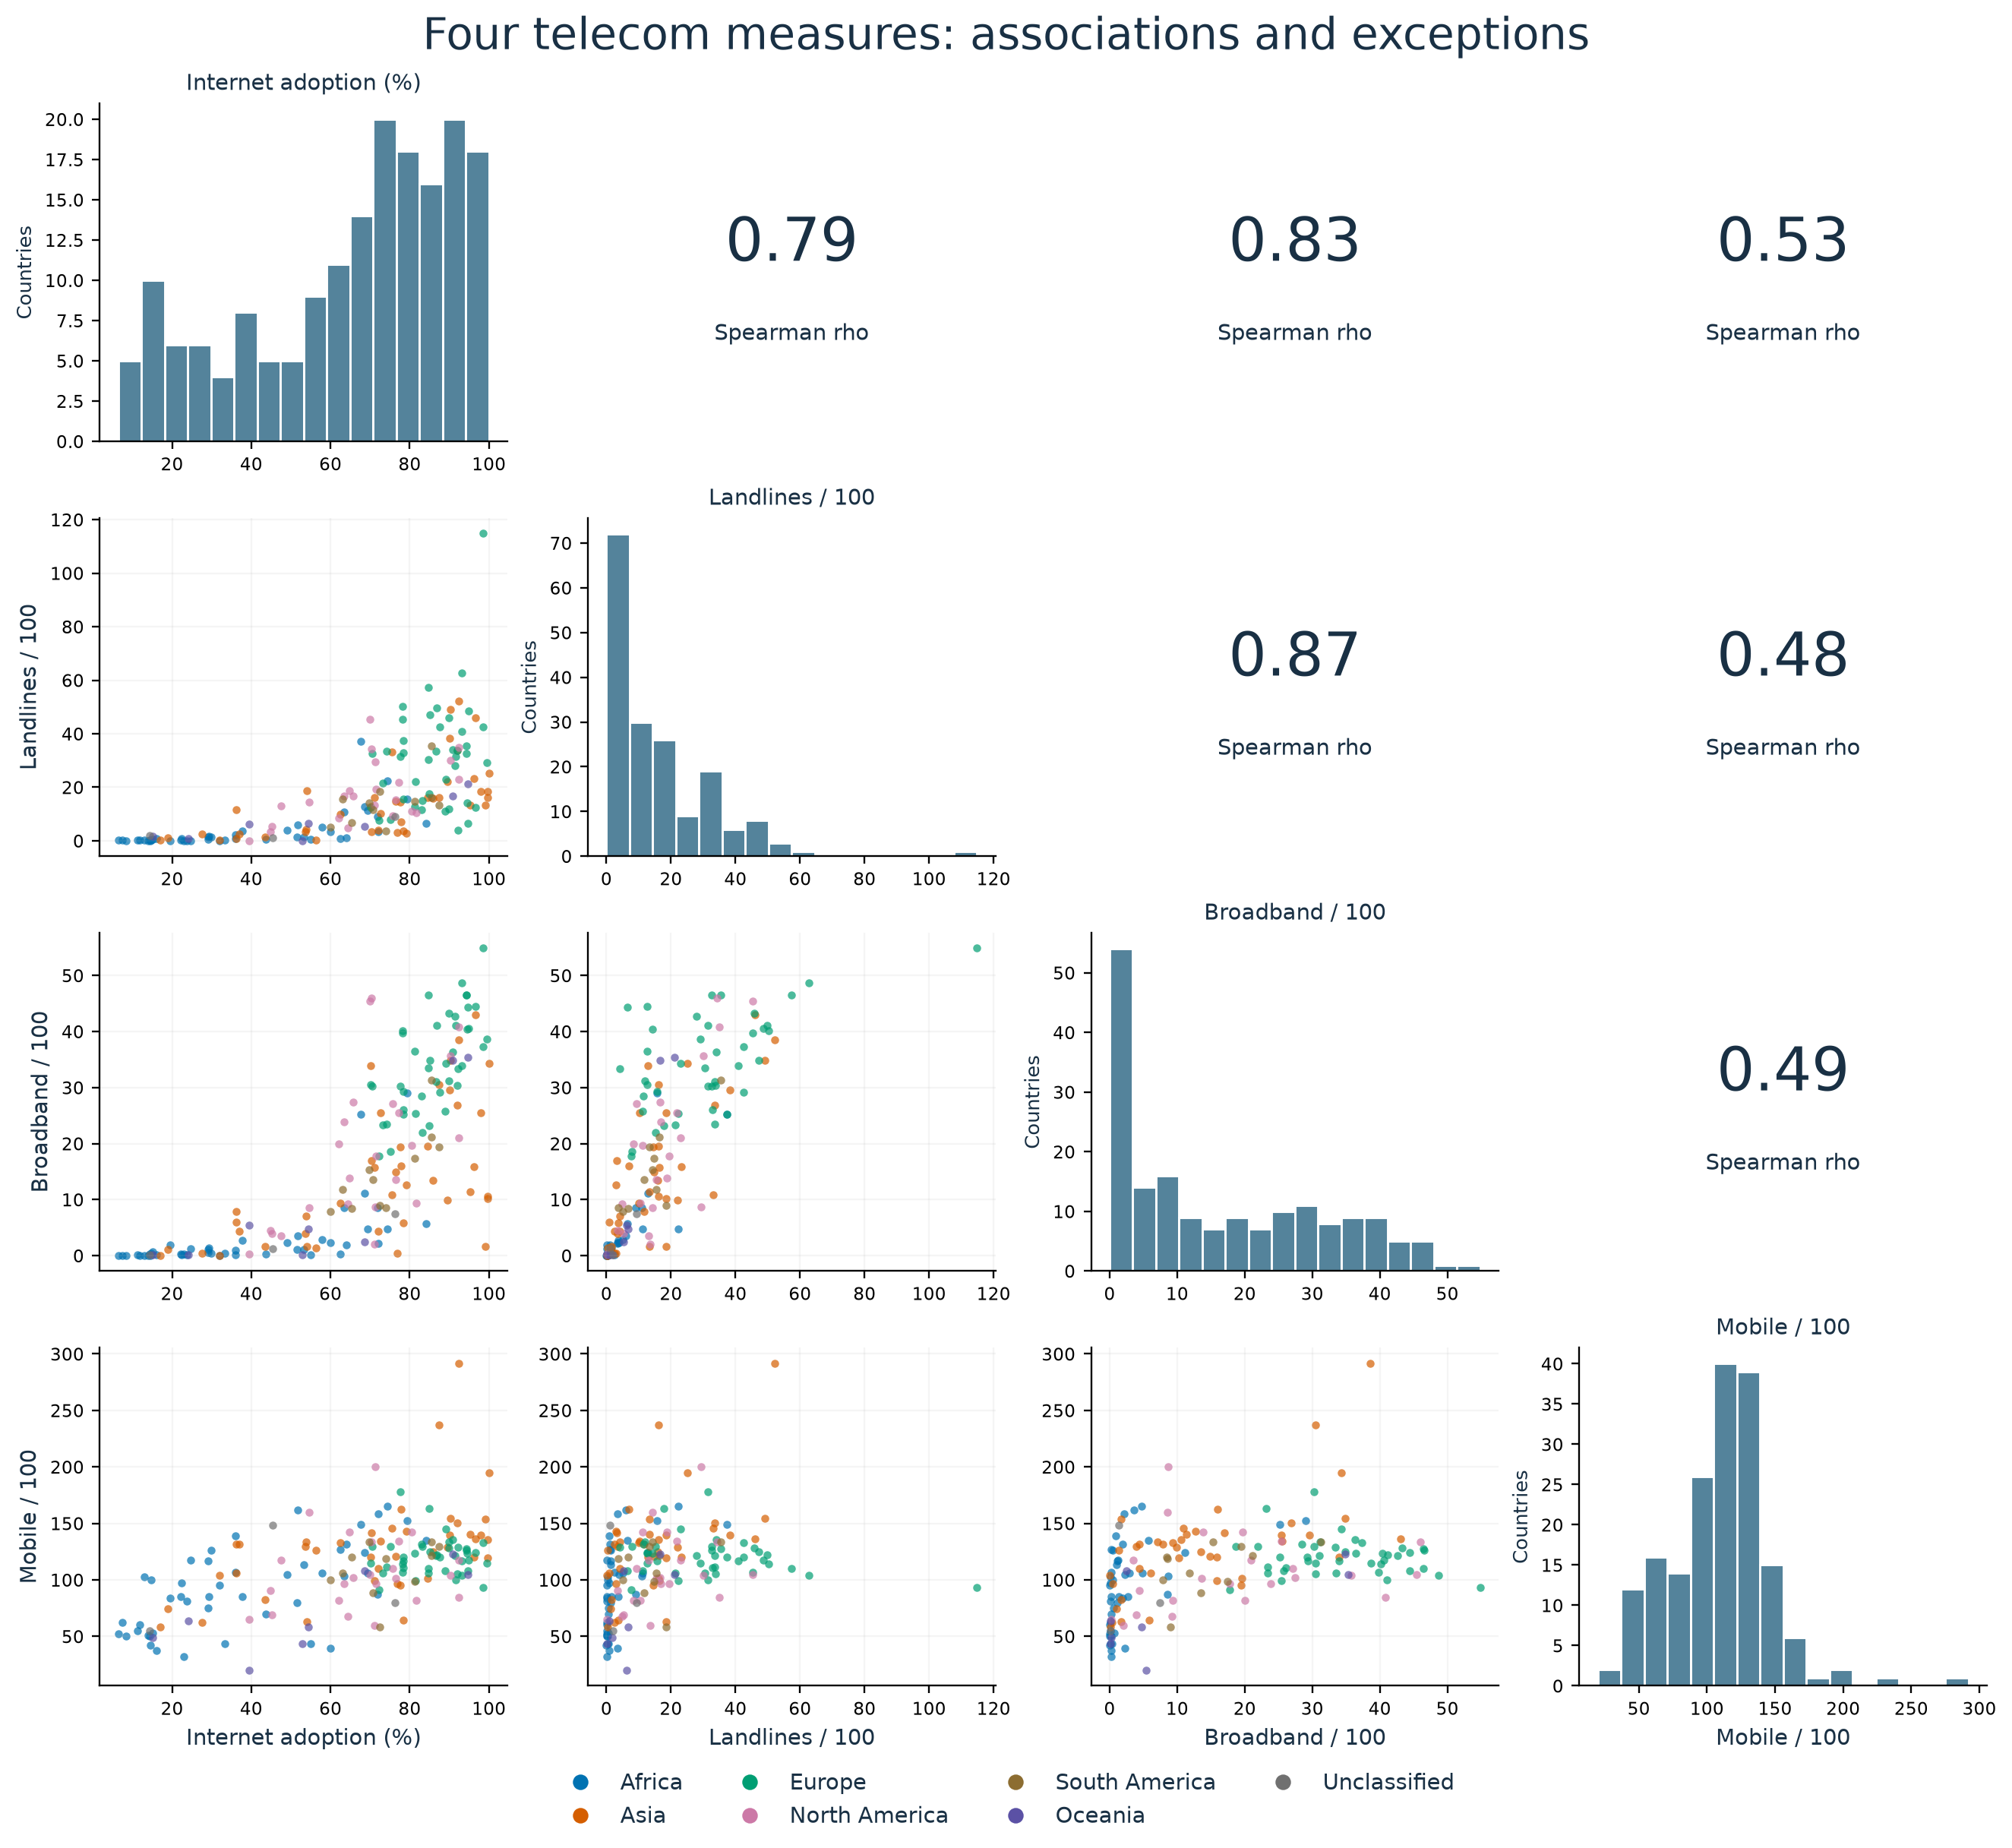
\includegraphics[width=\textwidth,height=0.62\textheight,keepaspectratio]{Fig7.png}

\caption{Pairwise associations coexist with substantial profile exceptions. {\footnotesize \href{https://aithal007.github.io/DV_assignment2/figures.html\#fig7}{\textcolor{accent}{\underline{View figure and interpretation online}}}}}\label{fig:7}

\end{figure*}

\noindent\textit{How to read the graph.} n=175 matched countries. Diagonals show distributions; lower cells plot pairs, upper cells Spearman rank associations. Region colors identify context.

\paragraph{Question.} What does the complete set of pairwise relationships reveal?



\paragraph{Visual encoding.} Cohort: the same 175 countries complete in both 2015 and 2020; four other 2020-complete countries lack complete 2015 profiles. The four variables occupy the same row and column order: internet use, landlines, fixed broadband and mobile. Diagonal cells are country-count histograms. Below the diagonal, each dot is one country, with the column variable on the horizontal axis and the row variable on the vertical axis. Color shows region. Above the diagonal, the matching pair has its Spearman rank-correlation value. All cells use the same 175 countries in 2020.



\paragraph{Why this visualization.} The two adoption scatterplots in A1 already compared broadband and mobile. Restoring the full scatterplot matrix adds the four other pairs, the individual distributions and a common sample. Each relationship can be checked in its own scatter cell rather than inferred from a single correlation number. This also gives a position-based check on the four-variable parallel-coordinate profiles.



\paragraph{Interpretation.} The lower scatter cells show tighter upward ordering for broadband versus adoption (Spearman $r_s = 0.83$) than for mobile versus adoption ($r_s = 0.53$). Landlines and broadband have the strongest displayed pairwise rank association, about $r_s = 0.87$. The clouds and outlying countries qualify those coefficients: high adoption still occurs at low fixed-broadband values, and mobile subscriptions overlap widely.

All cells use the same 175 countries, so different sample membership does not explain the contrast. Diagonal distributions also show why a subscription count can exceed 100 per 100 people without being an adoption percentage. This tests the profiles seen in parallel coordinates using ordinary position axes. It supports an association between 2020 country levels, while leaving causal explanations and country-specific change unresolved.



\paragraph{Scope and reading note.} These are national comparisons for one year. The next figure examines changes between two years.



\takeaway{A correlation summarizes an association while hiding its exceptions and shape. The scatter cells show stronger adoption association with broadband than mobile, yet substantial variation remains. These endpoint associations do not identify the drivers of country progress.

}

\noindent\textit{Analytical recommendation.} Check scatter shapes and exceptions alongside correlation coefficients.

\subsection{Fig. 8: Country levels and country gains tell different stories}

\begin{figure*}[!tb]\centering

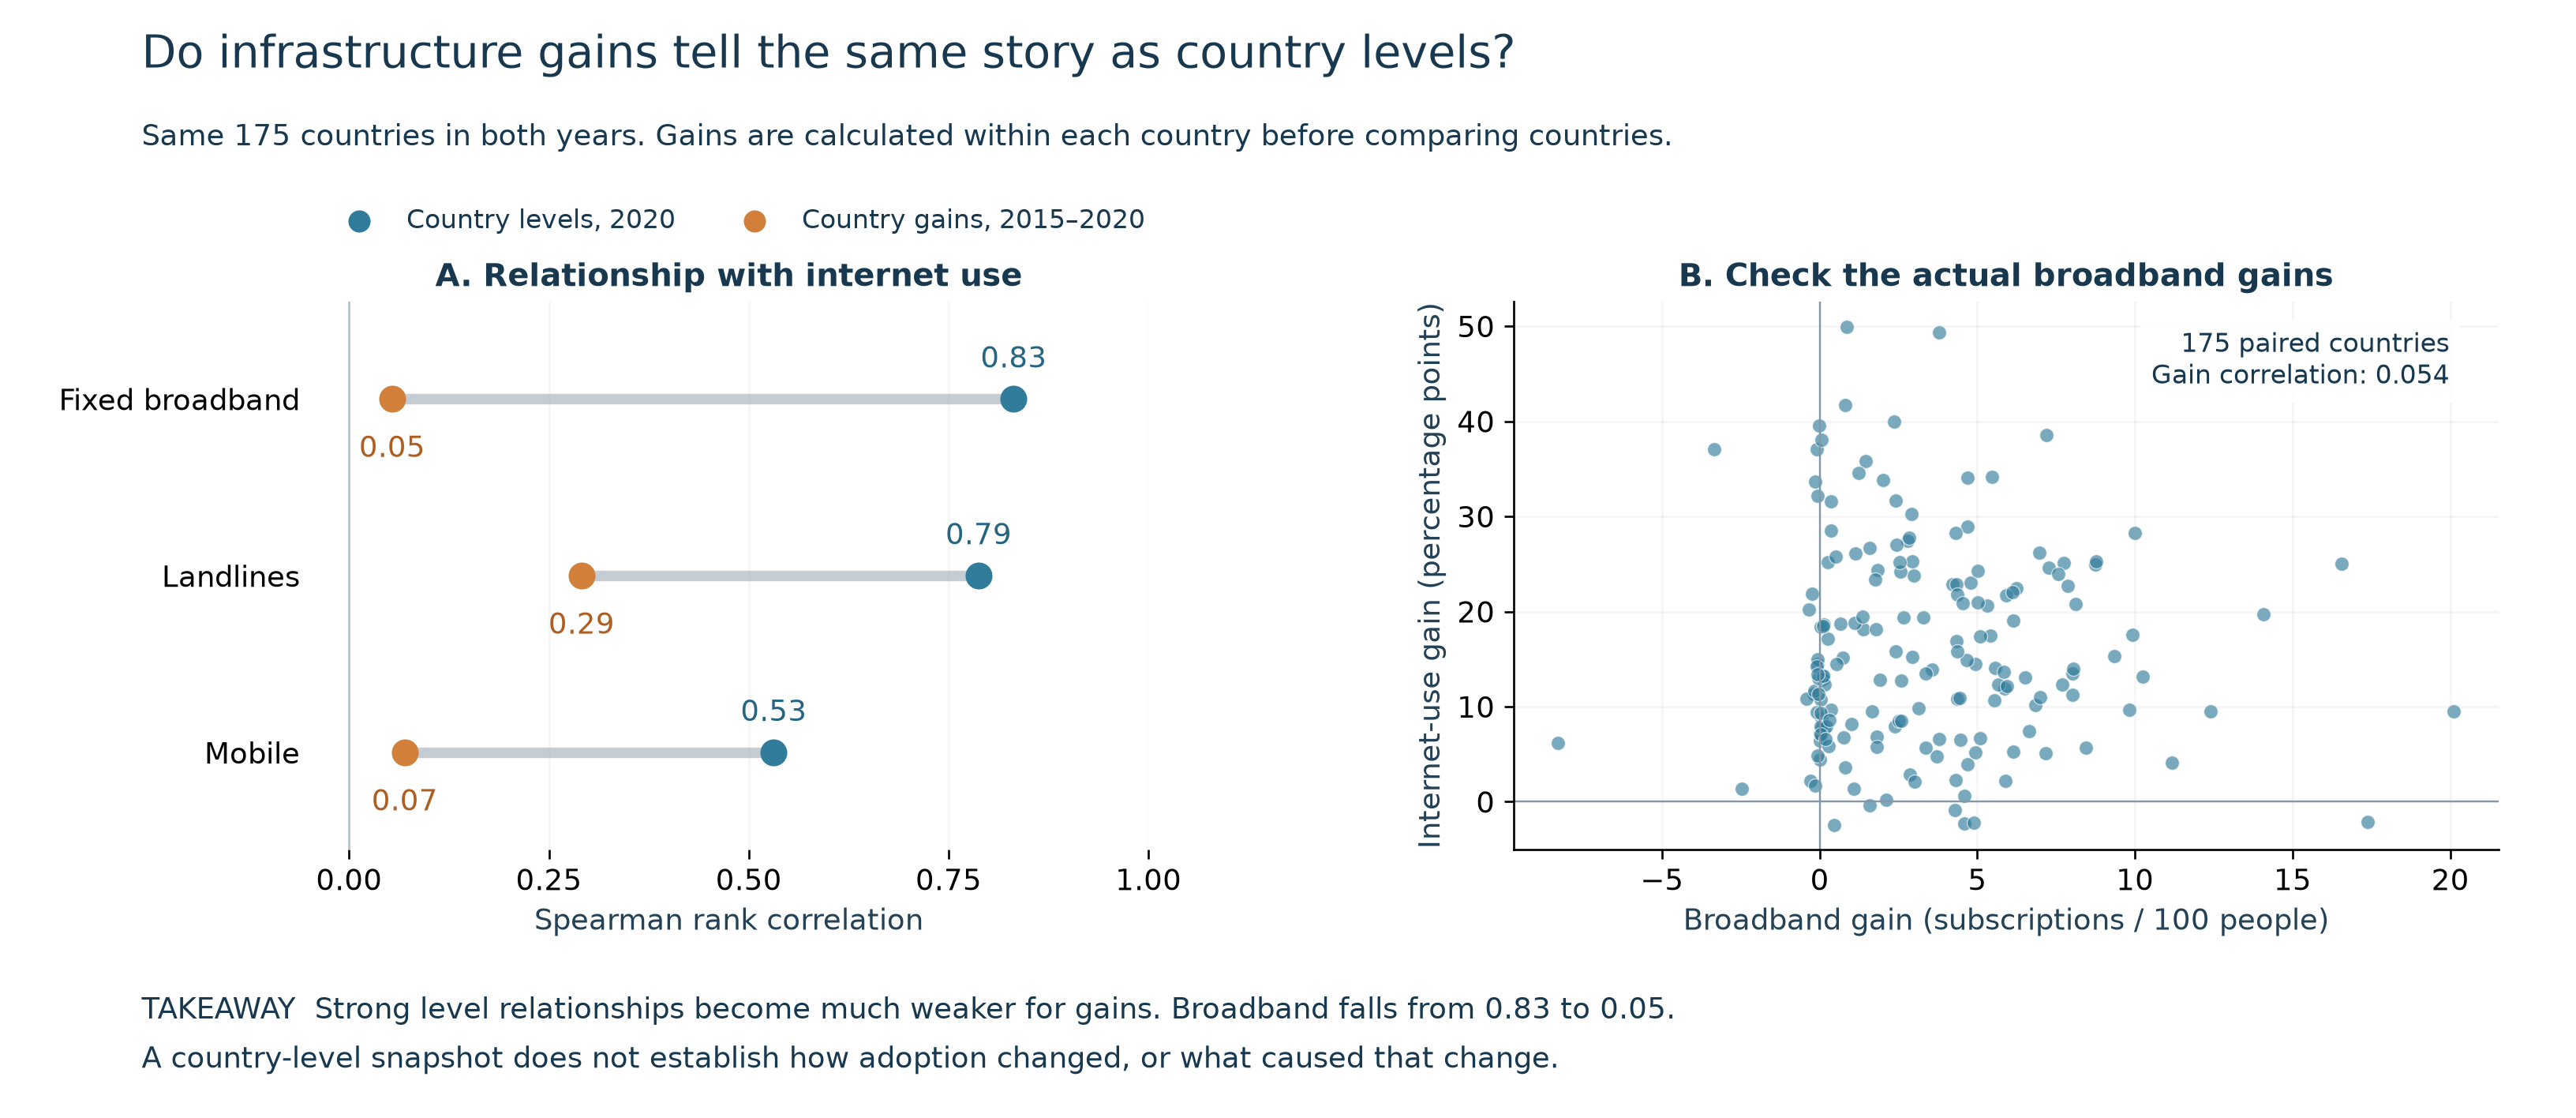
\includegraphics[width=\textwidth,height=0.49\textheight,keepaspectratio]{Fig8.png}

\caption{Strong endpoint association does not describe paired gains. {\footnotesize \href{https://aithal007.github.io/DV_assignment2/figures.html\#fig8}{\textcolor{accent}{\underline{View figure and interpretation online}}}}}\label{fig:8}

\end{figure*}

\noindent\textit{How to read the graph.} n=175 matched countries. Left compares adoption associations for levels and paired gains; right plots actual broadband/adoption gains, preserving exceptions.

\paragraph{Question.} Does a strong relationship between country levels also hold for gains within the same countries?



\paragraph{Visual encoding.} Cohort: the same 175 countries complete in both 2015 and 2020; four other 2020-complete countries lack complete 2015 profiles. The left panel compares Spearman rank correlations with internet use for fixed broadband, landlines and mobile. Blue dots use 2020 country levels; orange dots use each country's 2020-minus-2015 gains. Each gray line joins the two correlations for one measure. The right panel shows the actual broadband and adoption gains, with one dot per country. Both comparisons use the same 175 complete country pairs. Correlation describes how consistently two variables increase together across countries.



\paragraph{Why this visualization.} Fig.~\ref{fig:7} shows relationships between country levels. Repeating the comparison after calculating each country's gain tests whether that snapshot relationship carries over to progress. The paired-dot chart compares all three measures without repeating six scatterplots. The broadband-gain scatterplot keeps the underlying observations visible, so the coefficients can be checked against the shape of the data.



\paragraph{Interpretation.} Across the same 175 countries, broadband-adoption rank association falls from $r_s = 0.831$ ($p < 0.001$) in 2020 cross-sectional levels to $r_s = 0.054$ ($p = 0.48$) in paired 2015-2020 gains. The gain scatter lacks the ordered upward pattern suggested by the endpoint coefficient. Landline and mobile rank associations similarly weaken, from $r_s = 0.79$ to $r_s = 0.29$ ($p < 0.001$) and $r_s = 0.53$ to $r_s = 0.07$ ($p = 0.35$).

A floor effect operates in broadband gains: numerous developing countries experienced near-zero broadband additions over 2015-2020, mechanically attenuating rank correlation. Landline subscriptions declined in many countries over the same period ($r_s = +0.29$ for the gain-versus-adoption gain correlation), though this positive association is weaker than for country levels. High-baseline countries also have less possible gain due to the 100\% ceiling. The figure demonstrates that cross-sectional snapshots cannot substitute for paired changes.



\paragraph{Scope and reading note.} Gain correlations describe differences in five-year changes across the paired countries; they are not correlations of every annual observation within a country.



\takeaway{Countries that have more broadband tend to have higher adoption, but countries gaining more broadband do not show the same ordering of adoption gains. The fall from $r_s = 0.83$ to $r_s = 0.05$ exposes why a cross-country snapshot cannot substitute for paired change.

}

\noindent\textit{Analytical recommendation.} Evaluate paired gains directly; endpoint association cannot substitute for change analysis.

\subsection{Fig. 9: Internet users grouped by region}

\begin{figure*}[!tb]\centering

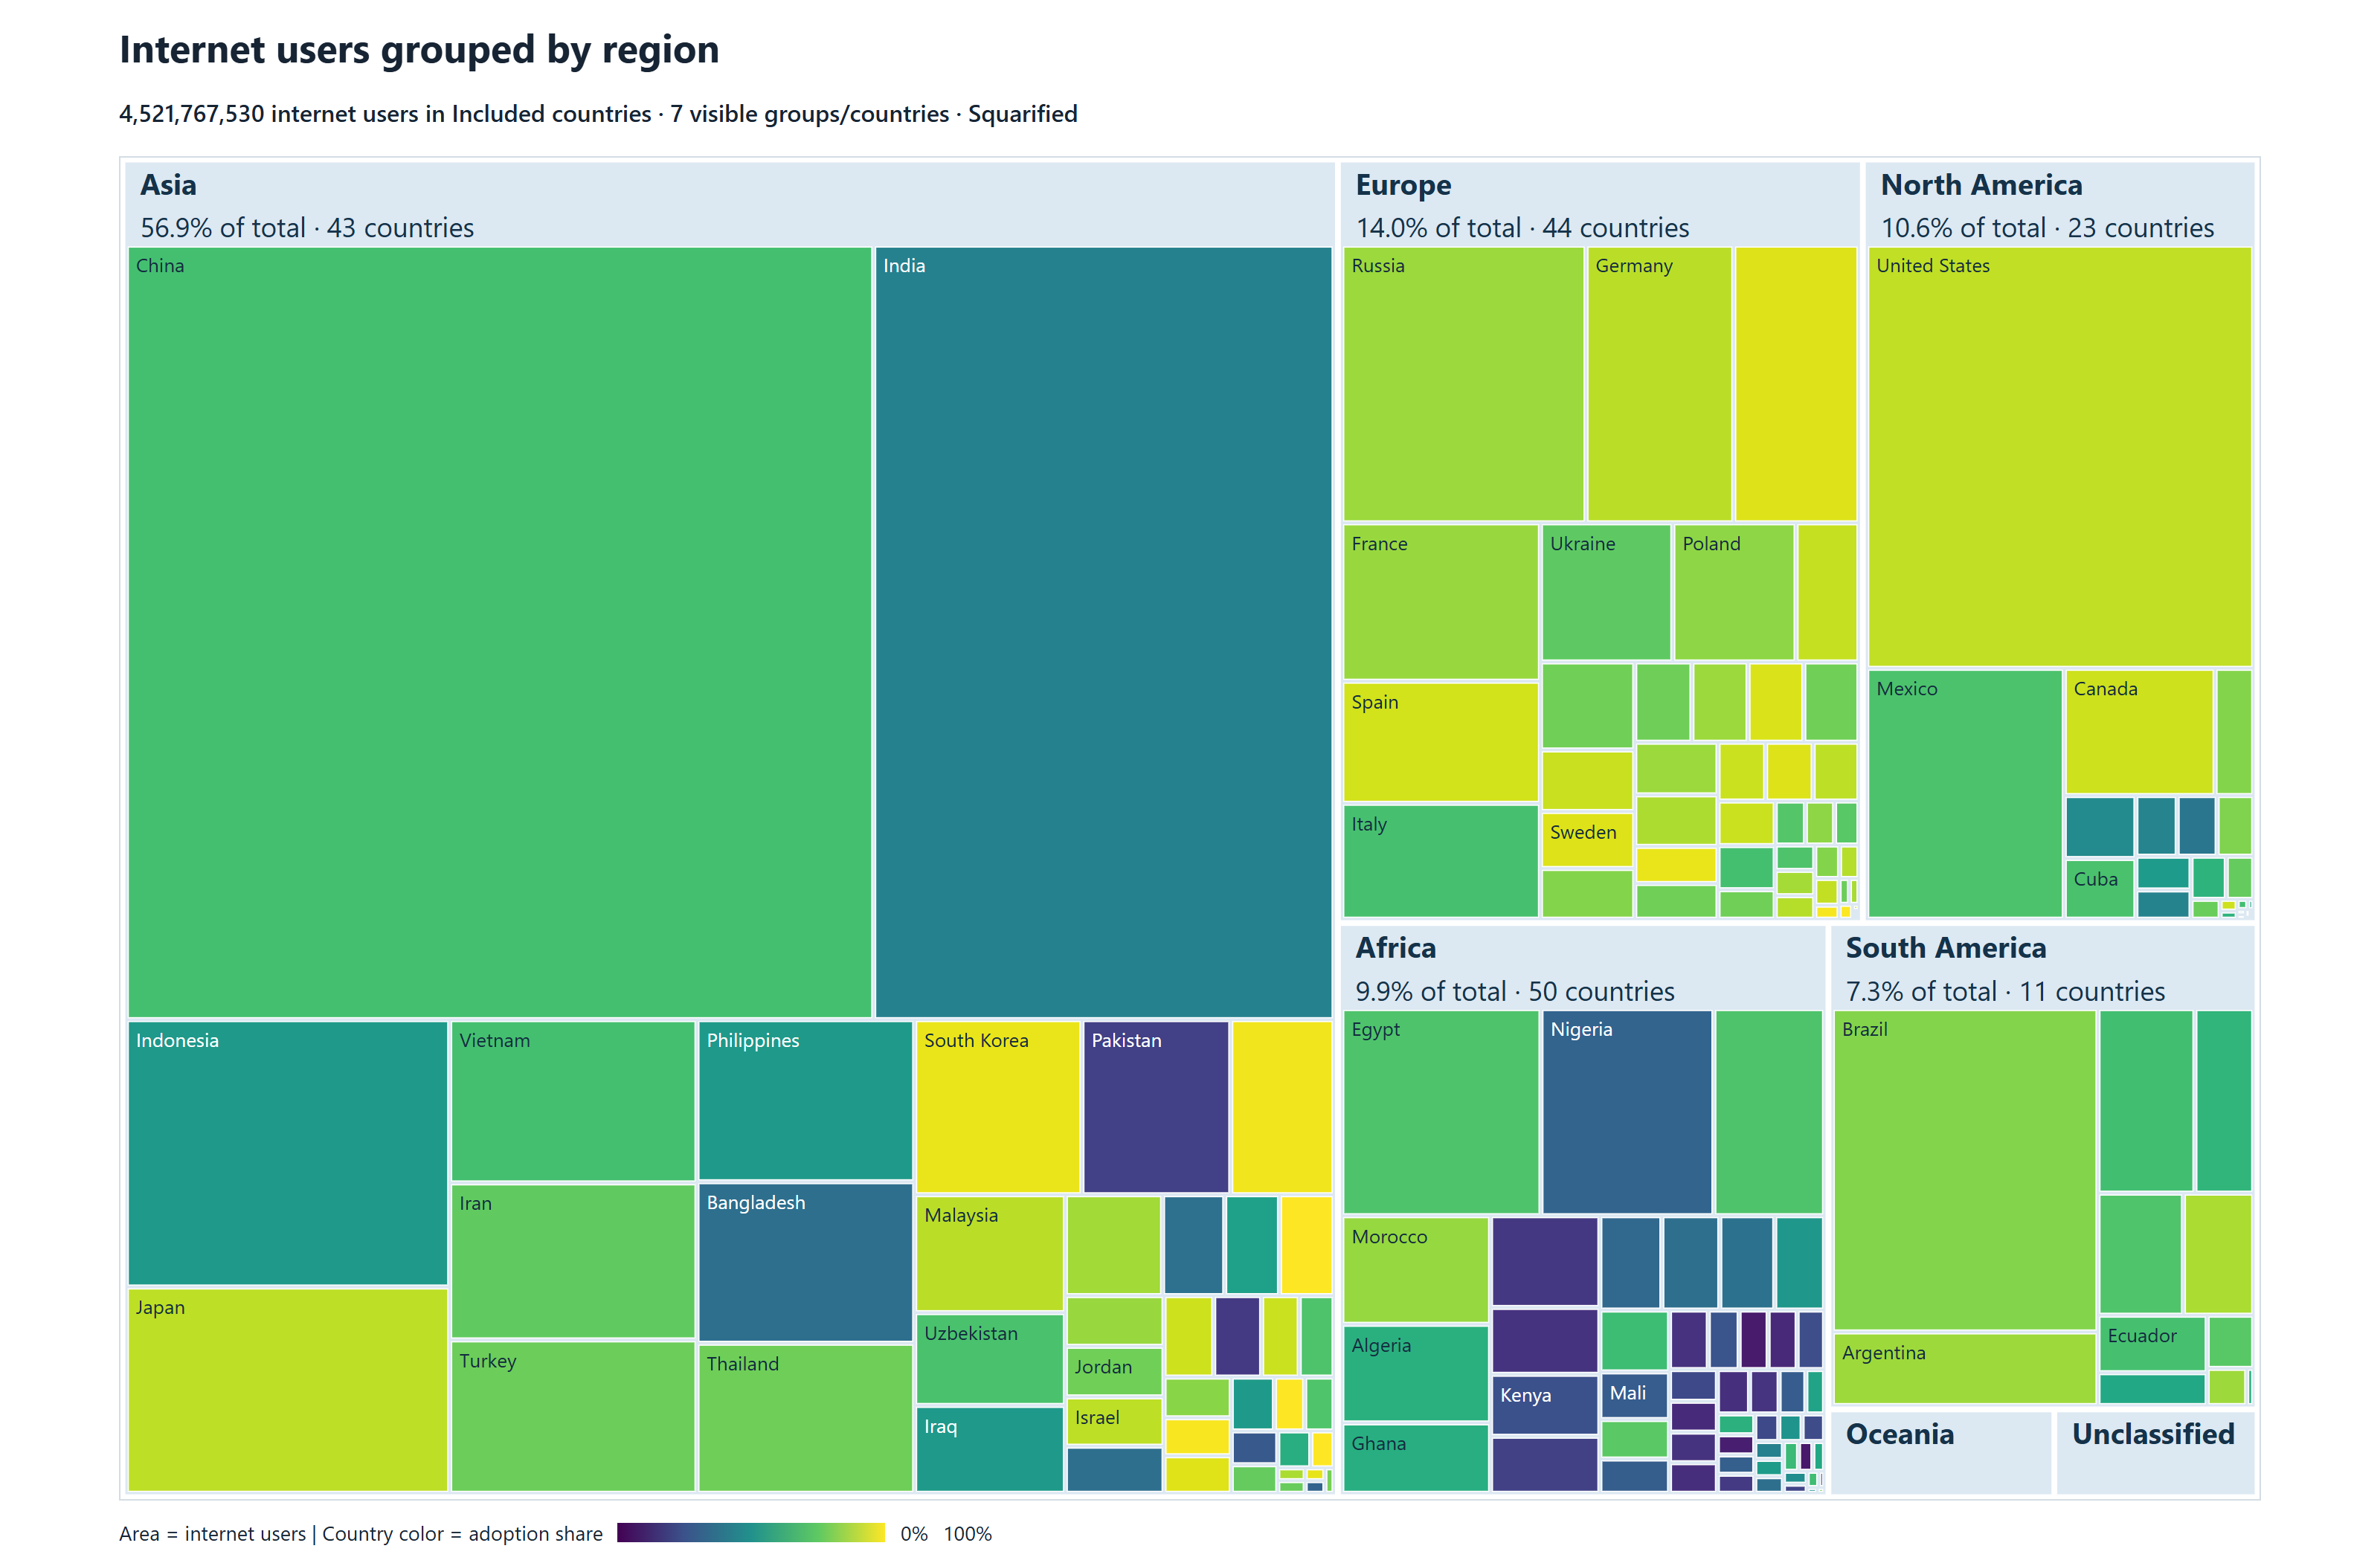
\includegraphics[width=\textwidth,height=0.49\textheight,keepaspectratio]{Fig9.png}

\caption{Large online-user populations can coexist with incomplete adoption. {\footnotesize \href{https://aithal007.github.io/DV_assignment2/web/treemap.html}{\textcolor{accent}{\underline{View live demonstration}}} \quad | \quad \href{https://aithal007.github.io/DV_assignment2/interactions.html\#treemap}{\textcolor{accent}{\underline{Full UI screenshot}}}}}\label{fig:9}

\end{figure*}

\noindent\textit{How to read the graph.} n=184 countries. Region-first rectangles sum included users; country colors show adoption share. Zoom changes the displayed subset, not the underlying values.

\paragraph{Question.} Where are the included internet users concentrated?



\paragraph{Visual encoding.} Large rectangles are regions; smaller country rectangles sit inside them. Area shows the number of internet users. Country color shows the percentage of people online. Group headers show each region's share of the included total.



\paragraph{Why this visualization.} A country with a high internet-use rate can still have fewer users than a large country with a lower rate. The nested treemap separates these two quantities: area shows the count and color shows the rate. Region-first grouping answers where the included users live, while keeping countries inside their regions.



\paragraph{Interpretation.} Asia occupies about 56.9\% of the included internet-user total, compared with 14.0\% in Europe. China and India are large country rectangles because user counts are large; their colors can differ because adoption percentages measure a separate quantity. The total denominator is the same 184-country, 4,521,767,530-user sample, not an estimate covering every missing country.

This answers where included users are concentrated while showing why a large user population does not imply near-universal access. Zooming into Asia reveals country counts and rates hidden by its regional area. The live spatial-partition control also compares squarified rectangles with slice-and-dice strips; values and hierarchy remain fixed while geometry changes. Compare encoded values, not a country's apparent visual prominence alone.



\paragraph{Scope and reading note.} The total covers 184 countries with both required values. It is not a complete count for every country in the world.



\takeaway{A large internet-user count can coexist with incomplete population access. China has about 988.5 million included users at 70.1\% adoption, while India has about 608.8 million at 43.4\% (a 26.7 percentage-point adoption gap). Rectangle size alone says nothing about adoption percentage; read count area and country color together.

}

\noindent\textit{Analytical recommendation.} Read count and adoption share together when discussing access.

\subsection{Fig. 10: The same users grouped by adoption band}

\begin{figure*}[!tb]\centering

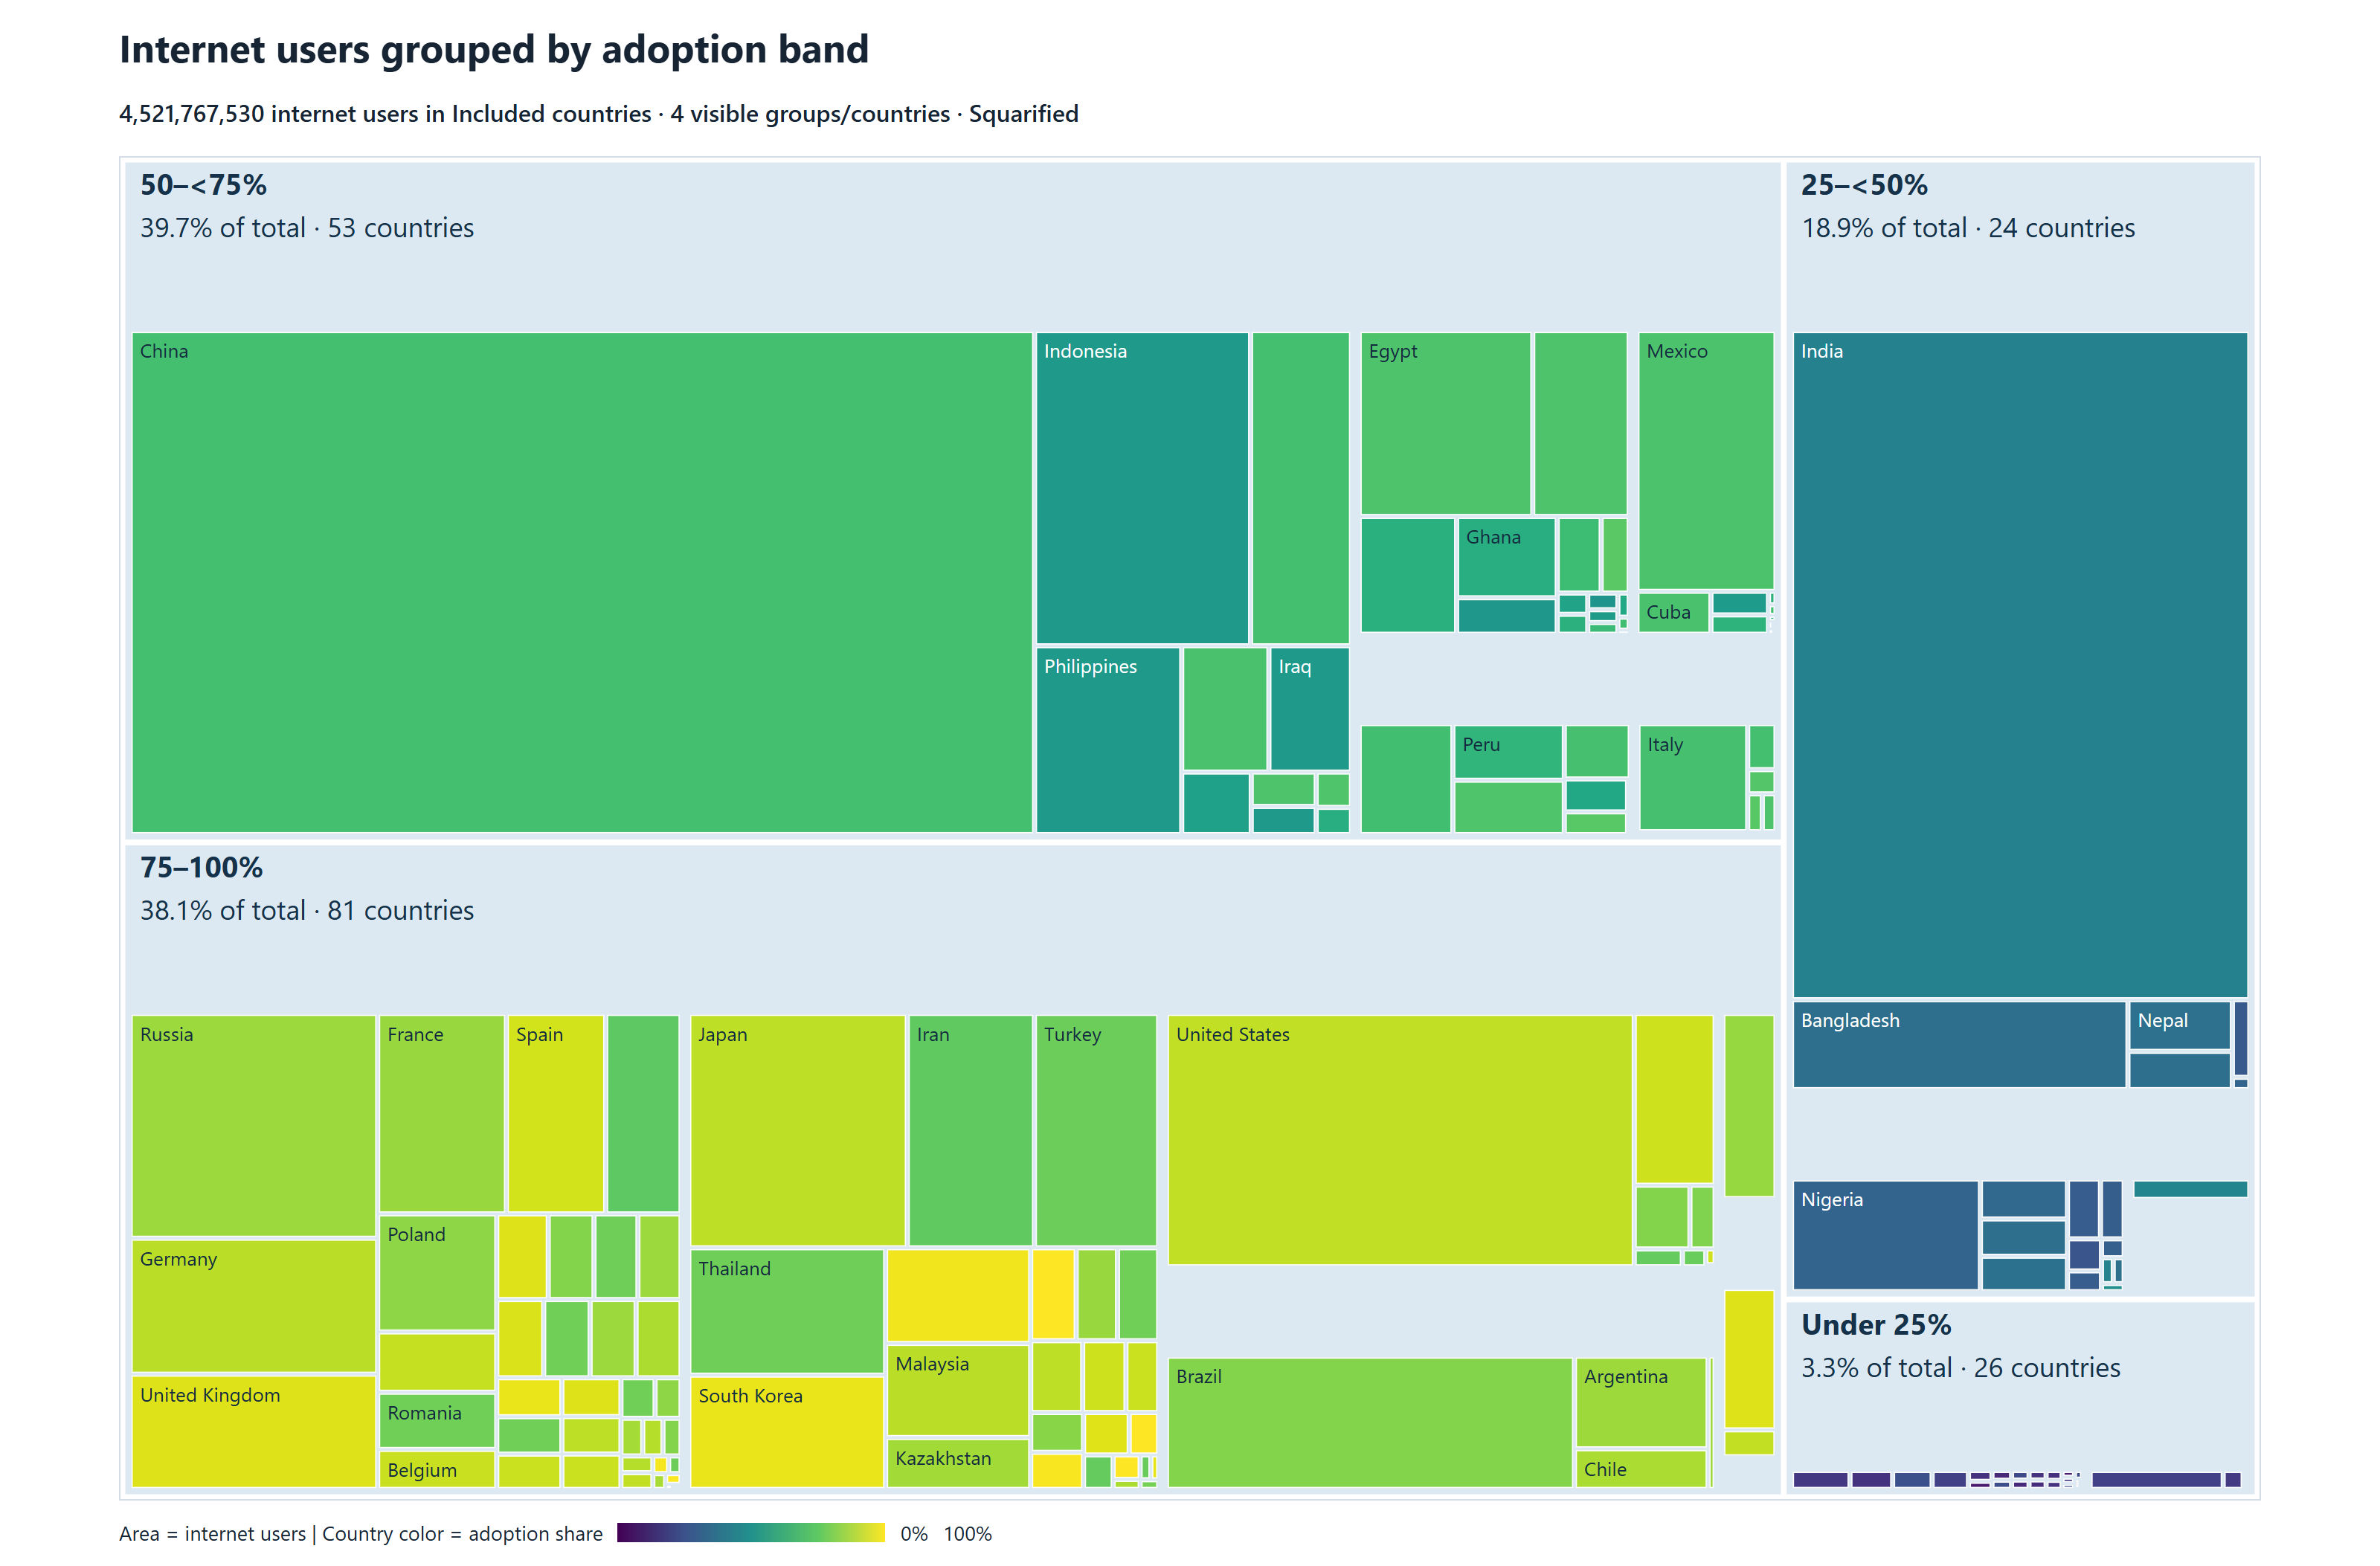
\includegraphics[width=\textwidth,height=0.49\textheight,keepaspectratio]{Fig10.png}

\caption{Hierarchy remodeling changes which composition is prominent, preserving the total. {\footnotesize \href{https://aithal007.github.io/DV_assignment2/web/treemap.html}{\textcolor{accent}{\underline{View live demonstration}}} \quad | \quad \href{https://aithal007.github.io/DV_assignment2/interactions.html\#treemap}{\textcolor{accent}{\underline{Full UI screenshot}}}}}\label{fig:10}

\end{figure*}

\noindent\textit{How to read the graph.} The same 184 leaves and user total are regrouped by adoption band, then region. Area remains online-user count; color remains adoption share.

\paragraph{Question.} Does changing the hierarchy change the comparison?



\paragraph{Visual encoding.} This treemap uses the same 184 countries and total as Fig.~\ref{fig:9}. It first groups countries by internet-use band, then by region. Area still shows user count and country color still shows internet use.



\paragraph{Why this visualization.} The first treemap makes regional size prominent. Reversing the hierarchy asks which adoption levels contain those users. Keeping the country data, total area and color scale fixed isolates the effect of grouping. The two trees therefore answer different questions with the same records.



\paragraph{Interpretation.} Moving adoption band to the top exposes a different composition of the same user total: the 50-below-75\% band contains about 39.7\% of included users, slightly more than the 38.1\% in the 75-100\% band. Thus a large share of online people live in countries where a substantial part of the population remains offline.

No country values change when the hierarchy switches. The difference from the region-first view comes from which grouping is made visually prominent. This is evidence that aggregation design changes the question a summary answers. A rectangle represents online users, not offline population, so the plot does not directly count the access shortfall. The live partitioning comparison changes shapes only; zooming changes the displayed denominator, which is stated in the status and breadcrumb.



\paragraph{Scope and reading note.} Adoption bands are chosen categories. The browser lets the reader zoom in and inspect exact country values.



\takeaway{The distribution of users across adoption levels becomes visible when the hierarchy changes. The 50-below-75\% band contains 39.7\% of included users, so many online users live where substantial access gaps remain. Grouping changes the question answered by the same values.

}

\noindent\textit{Analytical recommendation.} Keep the denominator fixed when comparing alternative hierarchies.

\section{Progress, inequality and timing}

Fixed country identities distinguish progress from catch-up; distributions and trajectories retain the differences behind regional summaries.



\subsection{Fig. 11: Did countries that started behind catch up?}

\begin{figure*}[!tb]\centering

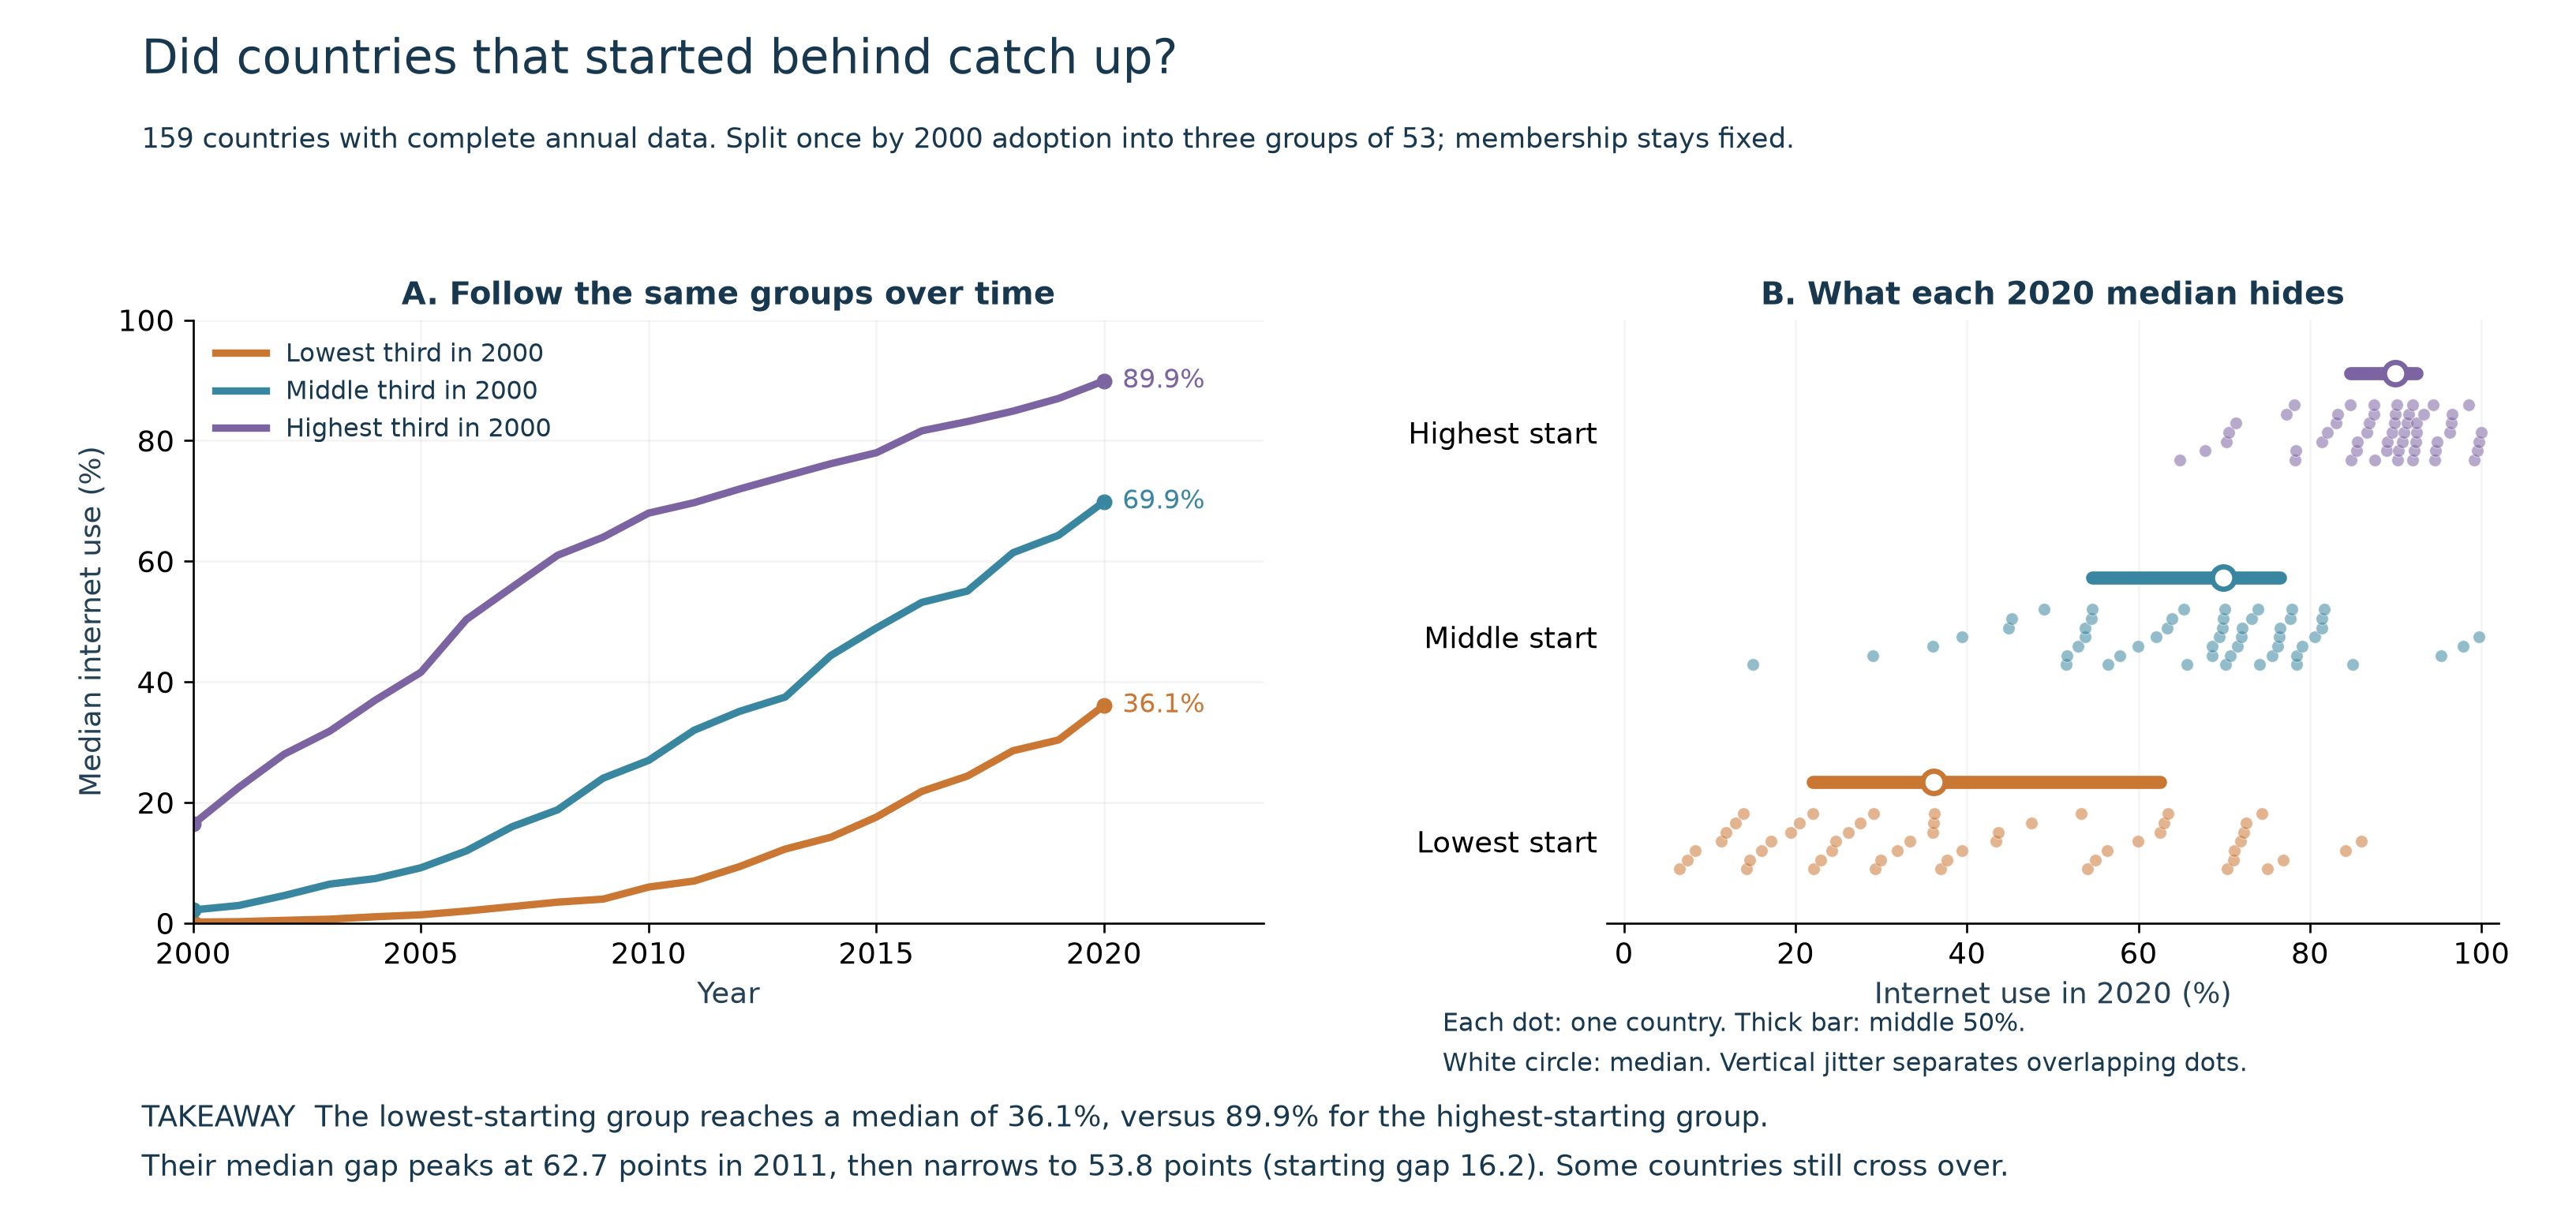
\includegraphics[width=\textwidth,height=0.54\textheight,keepaspectratio]{Fig11.png}

\caption{All fixed cohorts progress; the absolute gap peaks in 2011 then narrows, while remaining above its 2000 level in 2020. {\footnotesize \href{https://aithal007.github.io/DV_assignment2/figures.html\#fig11}{\textcolor{accent}{\underline{View figure and interpretation online}}}}}\label{fig:11}

\end{figure*}

\noindent\textit{How to read the graph.} The same 159 countries remain in three cohorts fixed by 2000 adoption. Curves are yearly medians; endpoint dots and middle-half bars expose spread.

\paragraph{Question.} Did the countries with the lowest initial internet use catch up as overall adoption rose?



\paragraph{Visual encoding.} The 159 countries with complete 2000-2020 records are ranked once by their internet use in 2000 and divided into three groups of 53. Orange is the lowest starting third, blue the middle third and purple the highest third. Membership stays fixed in every year. The left panel follows each group's yearly median. The right panel shows every country's 2020 value; the thick bar spans the middle half and the white circle marks the median. Small vertical offsets separate overlapping country dots and have no data meaning.



\paragraph{Why this visualization.} Yearly distributions can improve even when the countries that started behind remain behind. Keeping the same initial groups follows those countries instead of replacing them with whichever countries occupy a percentile later. The median paths show the group contrast over time; the individual dots prevent a group summary from hiding exceptions. This complements the later ridgelines, which compare overall and regional distributions.



\paragraph{Interpretation.} All fixed cohorts progress, but the lowest-start group ends at a median 36.1\% adoption and the highest at 89.9\%. Their absolute median gap expanded from 16.2 percentage points in 2000 to a peak of 62.7 points in 2011, before narrowing to 53.8 points in 2020. Fixed 2000 membership establishes that this trajectory is not an artifact of shifting cohort boundaries; overlapping endpoint dots retain individual exceptions.

This non-monotonic trajectory is consistent with S-curve diffusion dynamics: early adoption accelerated rapidly in high-resource nations before encountering saturation ceilings (approaching 90\%), while lower-starting nations entered their steep growth phase after 2011. The chart establishes broad progress without absolute median catch-up over this interval; it does not establish that every definition of inequality worsens.



\paragraph{Scope and reading note.} Starting groups are chosen descriptive categories. A median path is a group summary, not the history of a single representative country.



\takeaway{Broad progress does not imply a monotonic catch-up path. The low-to-high fixed-cohort median gap rises from 16.2 in 2000 to a 62.7-point peak in 2011, then narrows to 53.8 in 2020. Fixed membership establishes that this path is not created by moving countries between groups.

}

\noindent\textit{Analytical recommendation.} Distinguish absolute catch-up from broad progress and from relative inequality.

\subsection{Fig. 12: Country differences inside each region}

\begin{figure*}[!tb]\centering

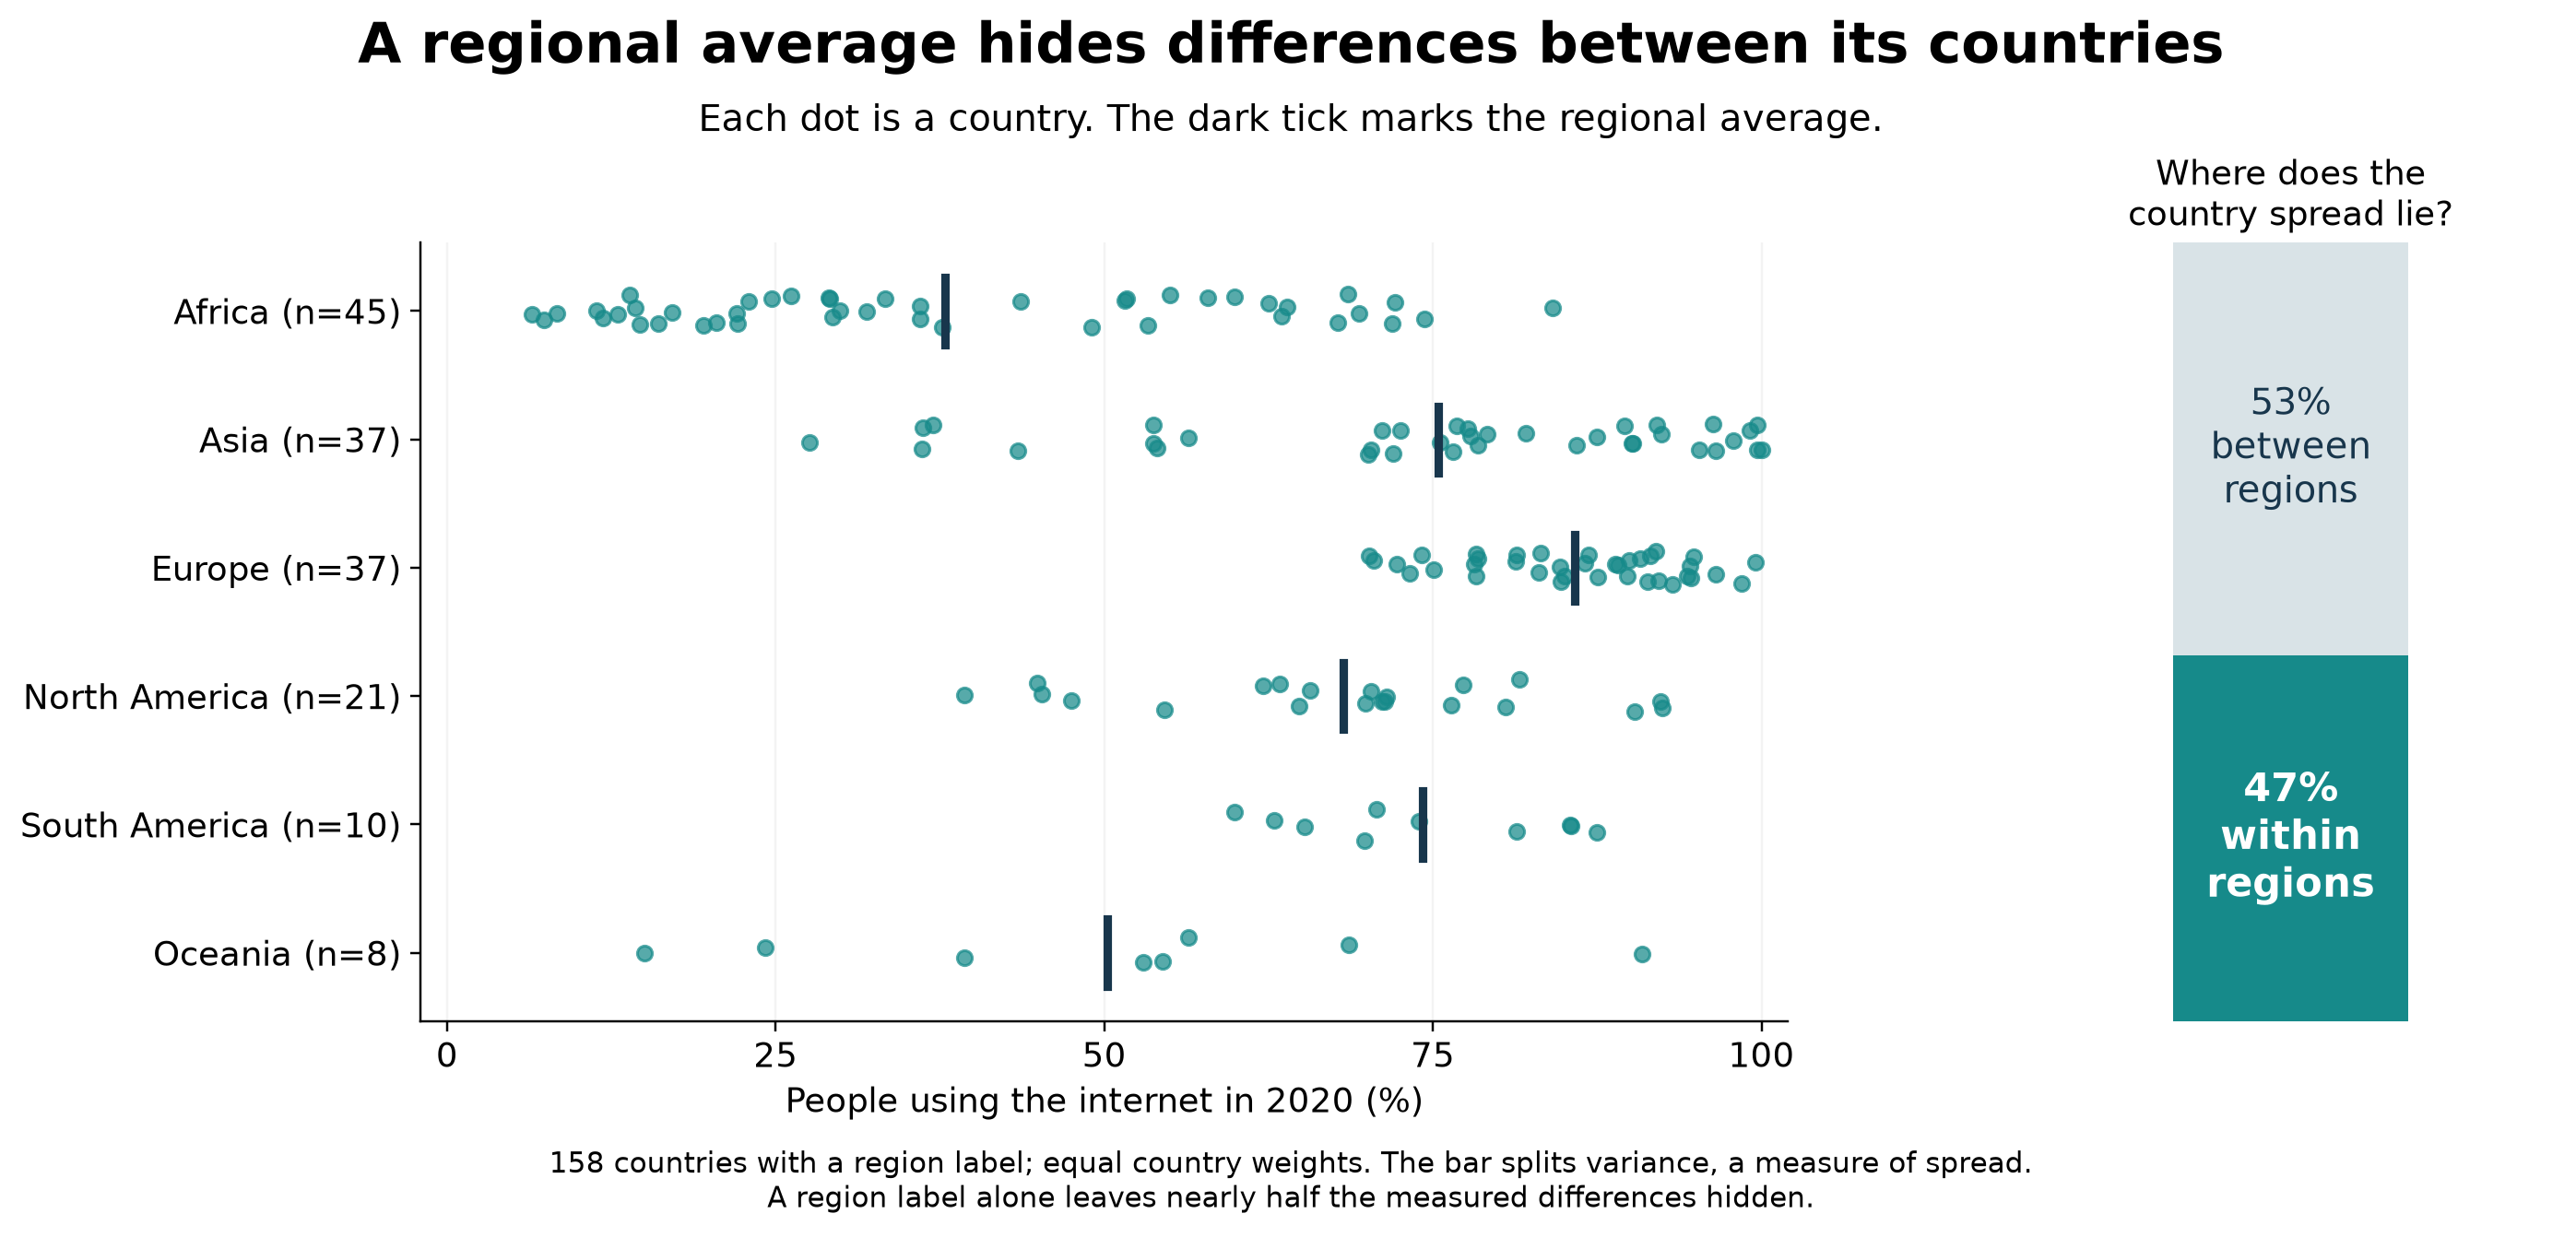
\includegraphics[width=\textwidth,height=0.49\textheight,keepaspectratio]{Fig12.png}

\caption{Regional averages conceal both within-region (47\%) and between-region (53\%) variation. {\footnotesize \href{https://aithal007.github.io/DV_assignment2/figures.html\#fig12}{\textcolor{accent}{\underline{View figure and interpretation online}}}}}\label{fig:12}

\end{figure*}

\noindent\textit{How to read the graph.} Each dot is one classified country; black ticks are regional averages. The variance bar partitions country-level variation within and between regions.

\paragraph{Question.} How much country variation does a regional average leave hidden?



\paragraph{Visual encoding.} Each dot shows one country's 2020 internet-use rate. A dark tick marks the regional average. The bar on the right divides the total spread into differences within regions and differences between regional averages.



\paragraph{Why this visualization.} A regional mean is one mark, even when its countries are far apart. Showing every country beside that mark reveals the spread directly. The variance split then gives a single numerical answer to how much of the total country variation sits inside regions. This extends the regional comparison without repeating A1's absolute-gap and ratio plots.



\paragraph{Interpretation.} The country dots spread widely around several regional averages. Variance decomposition assigns about 47\% of measured adoption variation to differences within regions and 53\% to differences between their means. This calculation uses the 158 region-classified members of the balanced country panel; the unclassified member is not silently assigned to a region.

The bars quantify what the dots make visible: a regional mean leaves nearly half of this measured country-level variation unresolved. Region therefore provides context without identifying the situation of each member. The decomposition weights regional mean contributions by country count and treats countries equally. It neither attributes 53\% of outcomes causally to region nor describes the share of people who have access. This is why regional progress must be interpreted alongside individual values.



\paragraph{Scope and reading note.} The split uses variance, a measure of spread, for 158 countries with known regions. Each country has equal weight.



\takeaway{Regional averages leave substantial country inequality unresolved: 47\% of measured variation is within regions and 53\% is between them. Both shares matter; the individual dots show why a regional label cannot stand in for its members.

}

\noindent\textit{Analytical recommendation.} Retain country-level spread when interpreting regional summaries.

\subsection{Fig. 13: Regional change and individual country gains}

\begin{figure*}[!tb]\centering

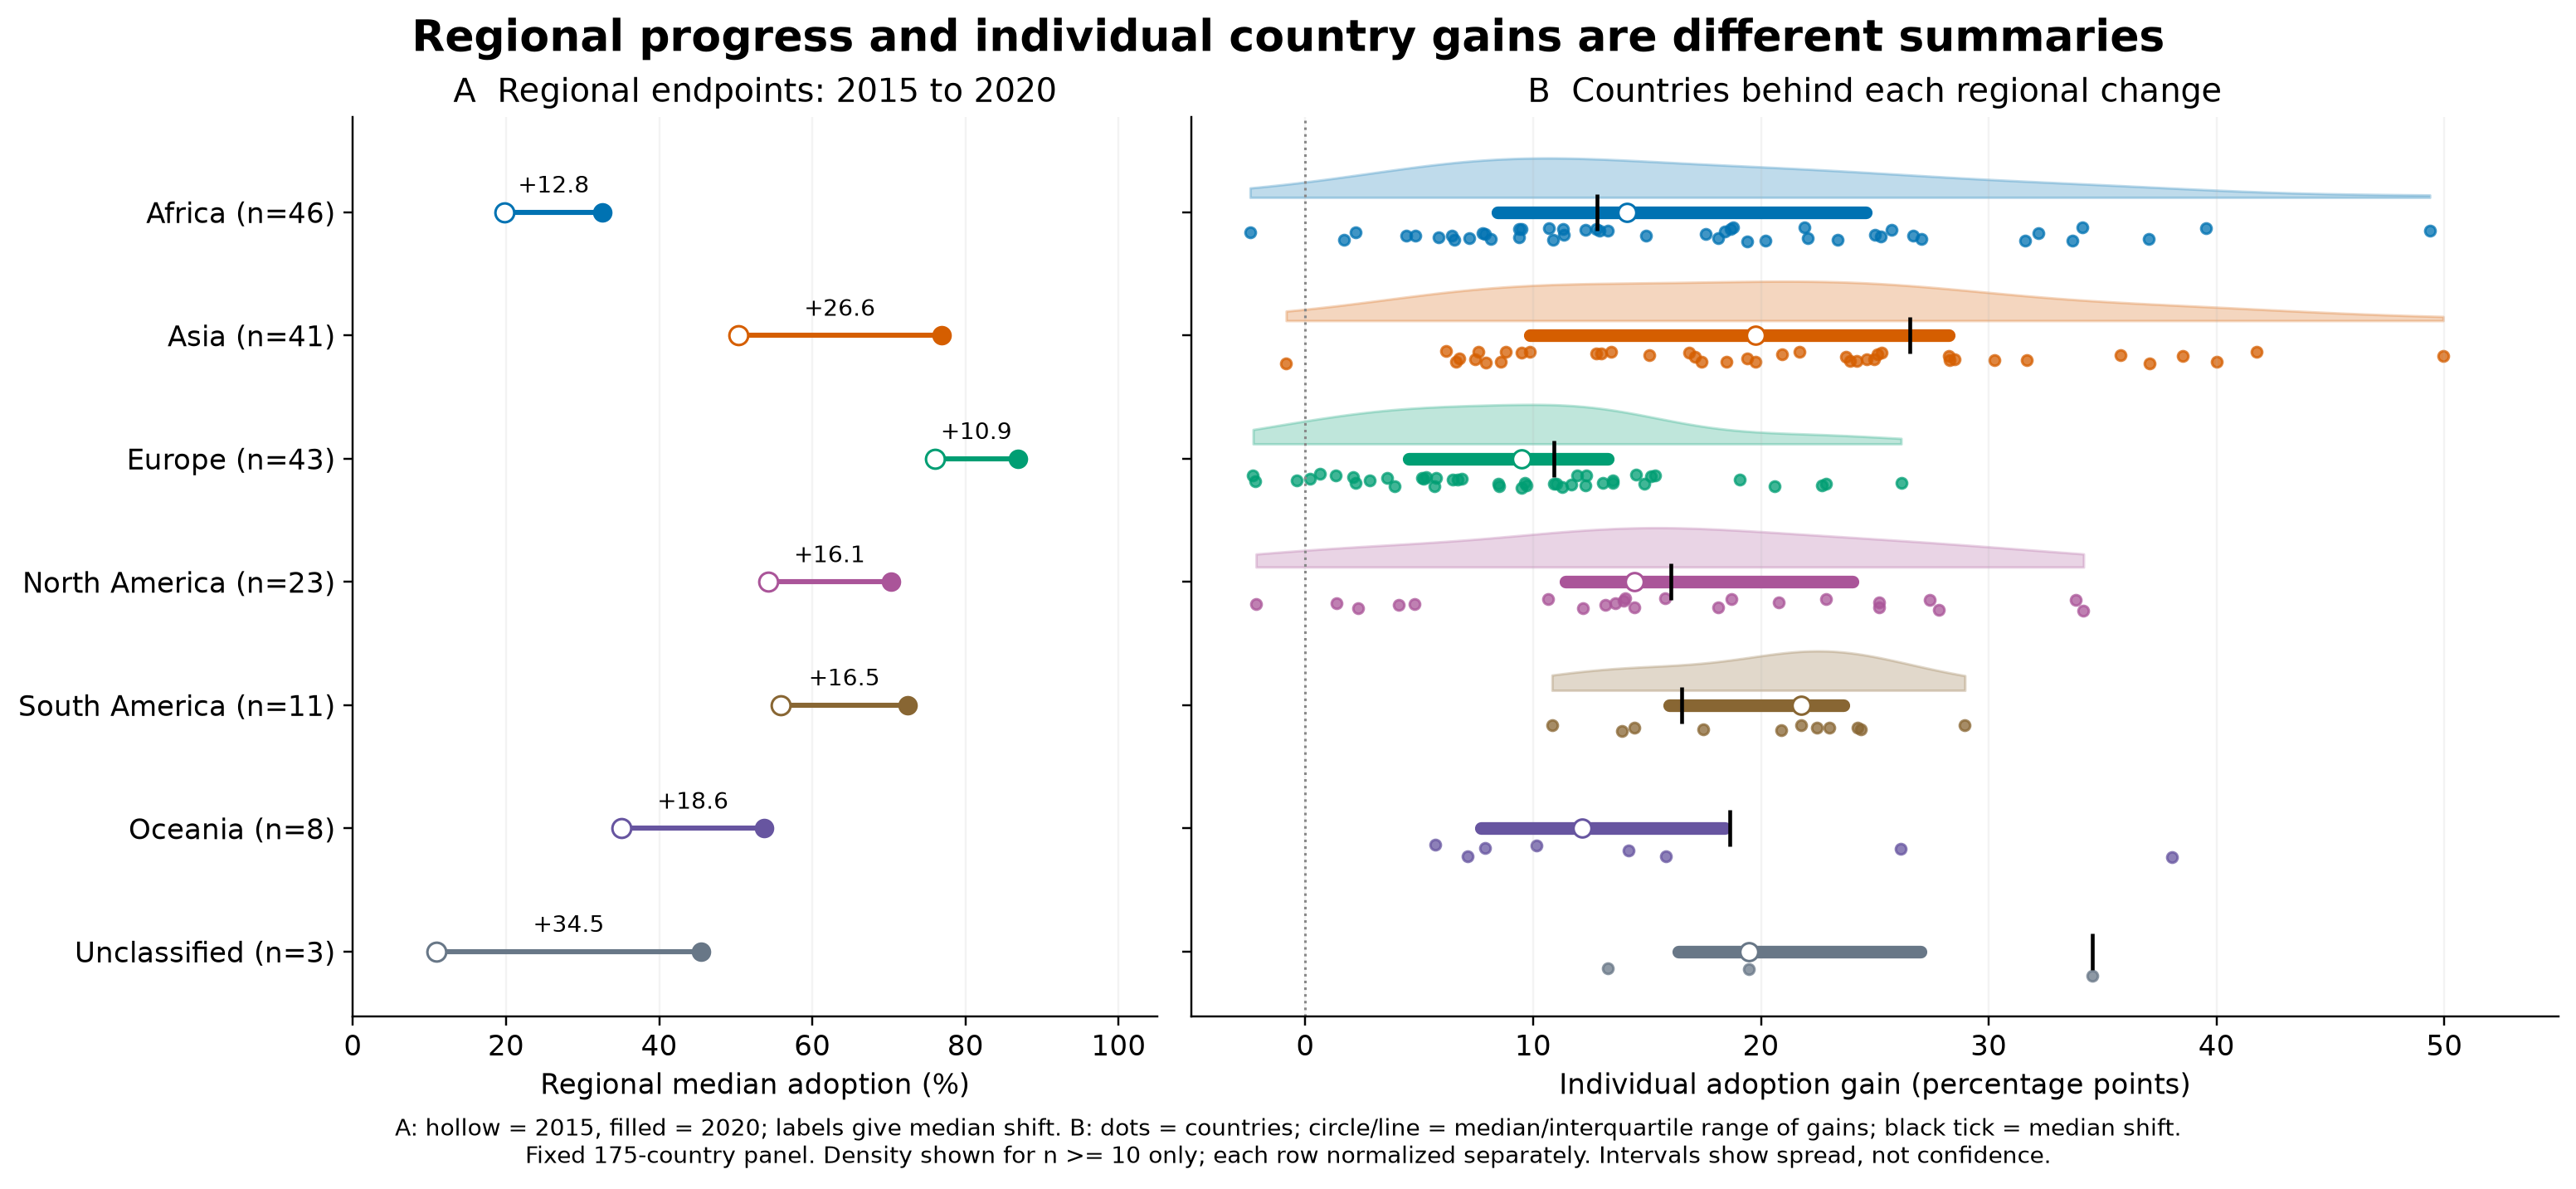
\includegraphics[width=\textwidth,height=0.49\textheight,keepaspectratio]{Fig13.png}

\caption{A regional median shift can differ from the median individual gain. {\footnotesize \href{https://aithal007.github.io/DV_assignment2/figures.html\#fig13}{\textcolor{accent}{\underline{View figure and interpretation online}}}}}\label{fig:13}

\end{figure*}

\noindent\textit{How to read the graph.} Paired 2015/2020 country gains appear beside regional endpoint medians. Black ticks mark median shifts; open markers mark median individual gains.

\paragraph{Question.} Does the change in a regional median describe a typical country's gain?



\paragraph{Visual encoding.} The left panel shows 2015 and 2020 regional medians. The right panel shows each country's own gain. A thick line marks the middle half of gains; the open circle is the median gain. The black tick repeats the shift in the regional median.



\paragraph{Why this visualization.} Subtracting two regional medians sounds like the typical country's gain, but the middle country can change between years. The paired endpoint view shows the regional summaries, and the gain view calculates change for each country first. Putting the two calculations together exposes the difference instead of asking the reader to infer it from separate tables.



\paragraph{Interpretation.} Asia's endpoint median shifts by 26.55 adoption points, but the median of its individual country gains is 19.75. South America reverses the relative comparison: its endpoint-median shift is 16.54 while its median country gain is 21.76. The visible separation between the black shift tick and open gain marker exposes the difference between these calculations.

The same countries are matched across 2015/2020. Subtracting two separately computed medians need not track one country's experience because the countries defining the middle may change. The gain dots additionally preserve Asia's wide range, about -0.84 to +49.94 points. This answers what a regional trend hides: both the distribution of progress and the distinction between summary movement and a typical paired change. Neither operation identifies causes.



\paragraph{Scope and reading note.} The spread lines describe variation between country gains. They are not confidence intervals.



\takeaway{A shift in a regional median is a different quantity from a typical country gain. Asia gives 26.55 versus 19.75 points. Calculate paired changes first when the question concerns individual progress; summarizing first can change the answer.

}

\noindent\textit{Analytical recommendation.} Calculate individual gains before interpreting a shift in regional medians.

\subsection{Fig. 14: Country horizon plots}

\begin{figure*}[!tb]\centering

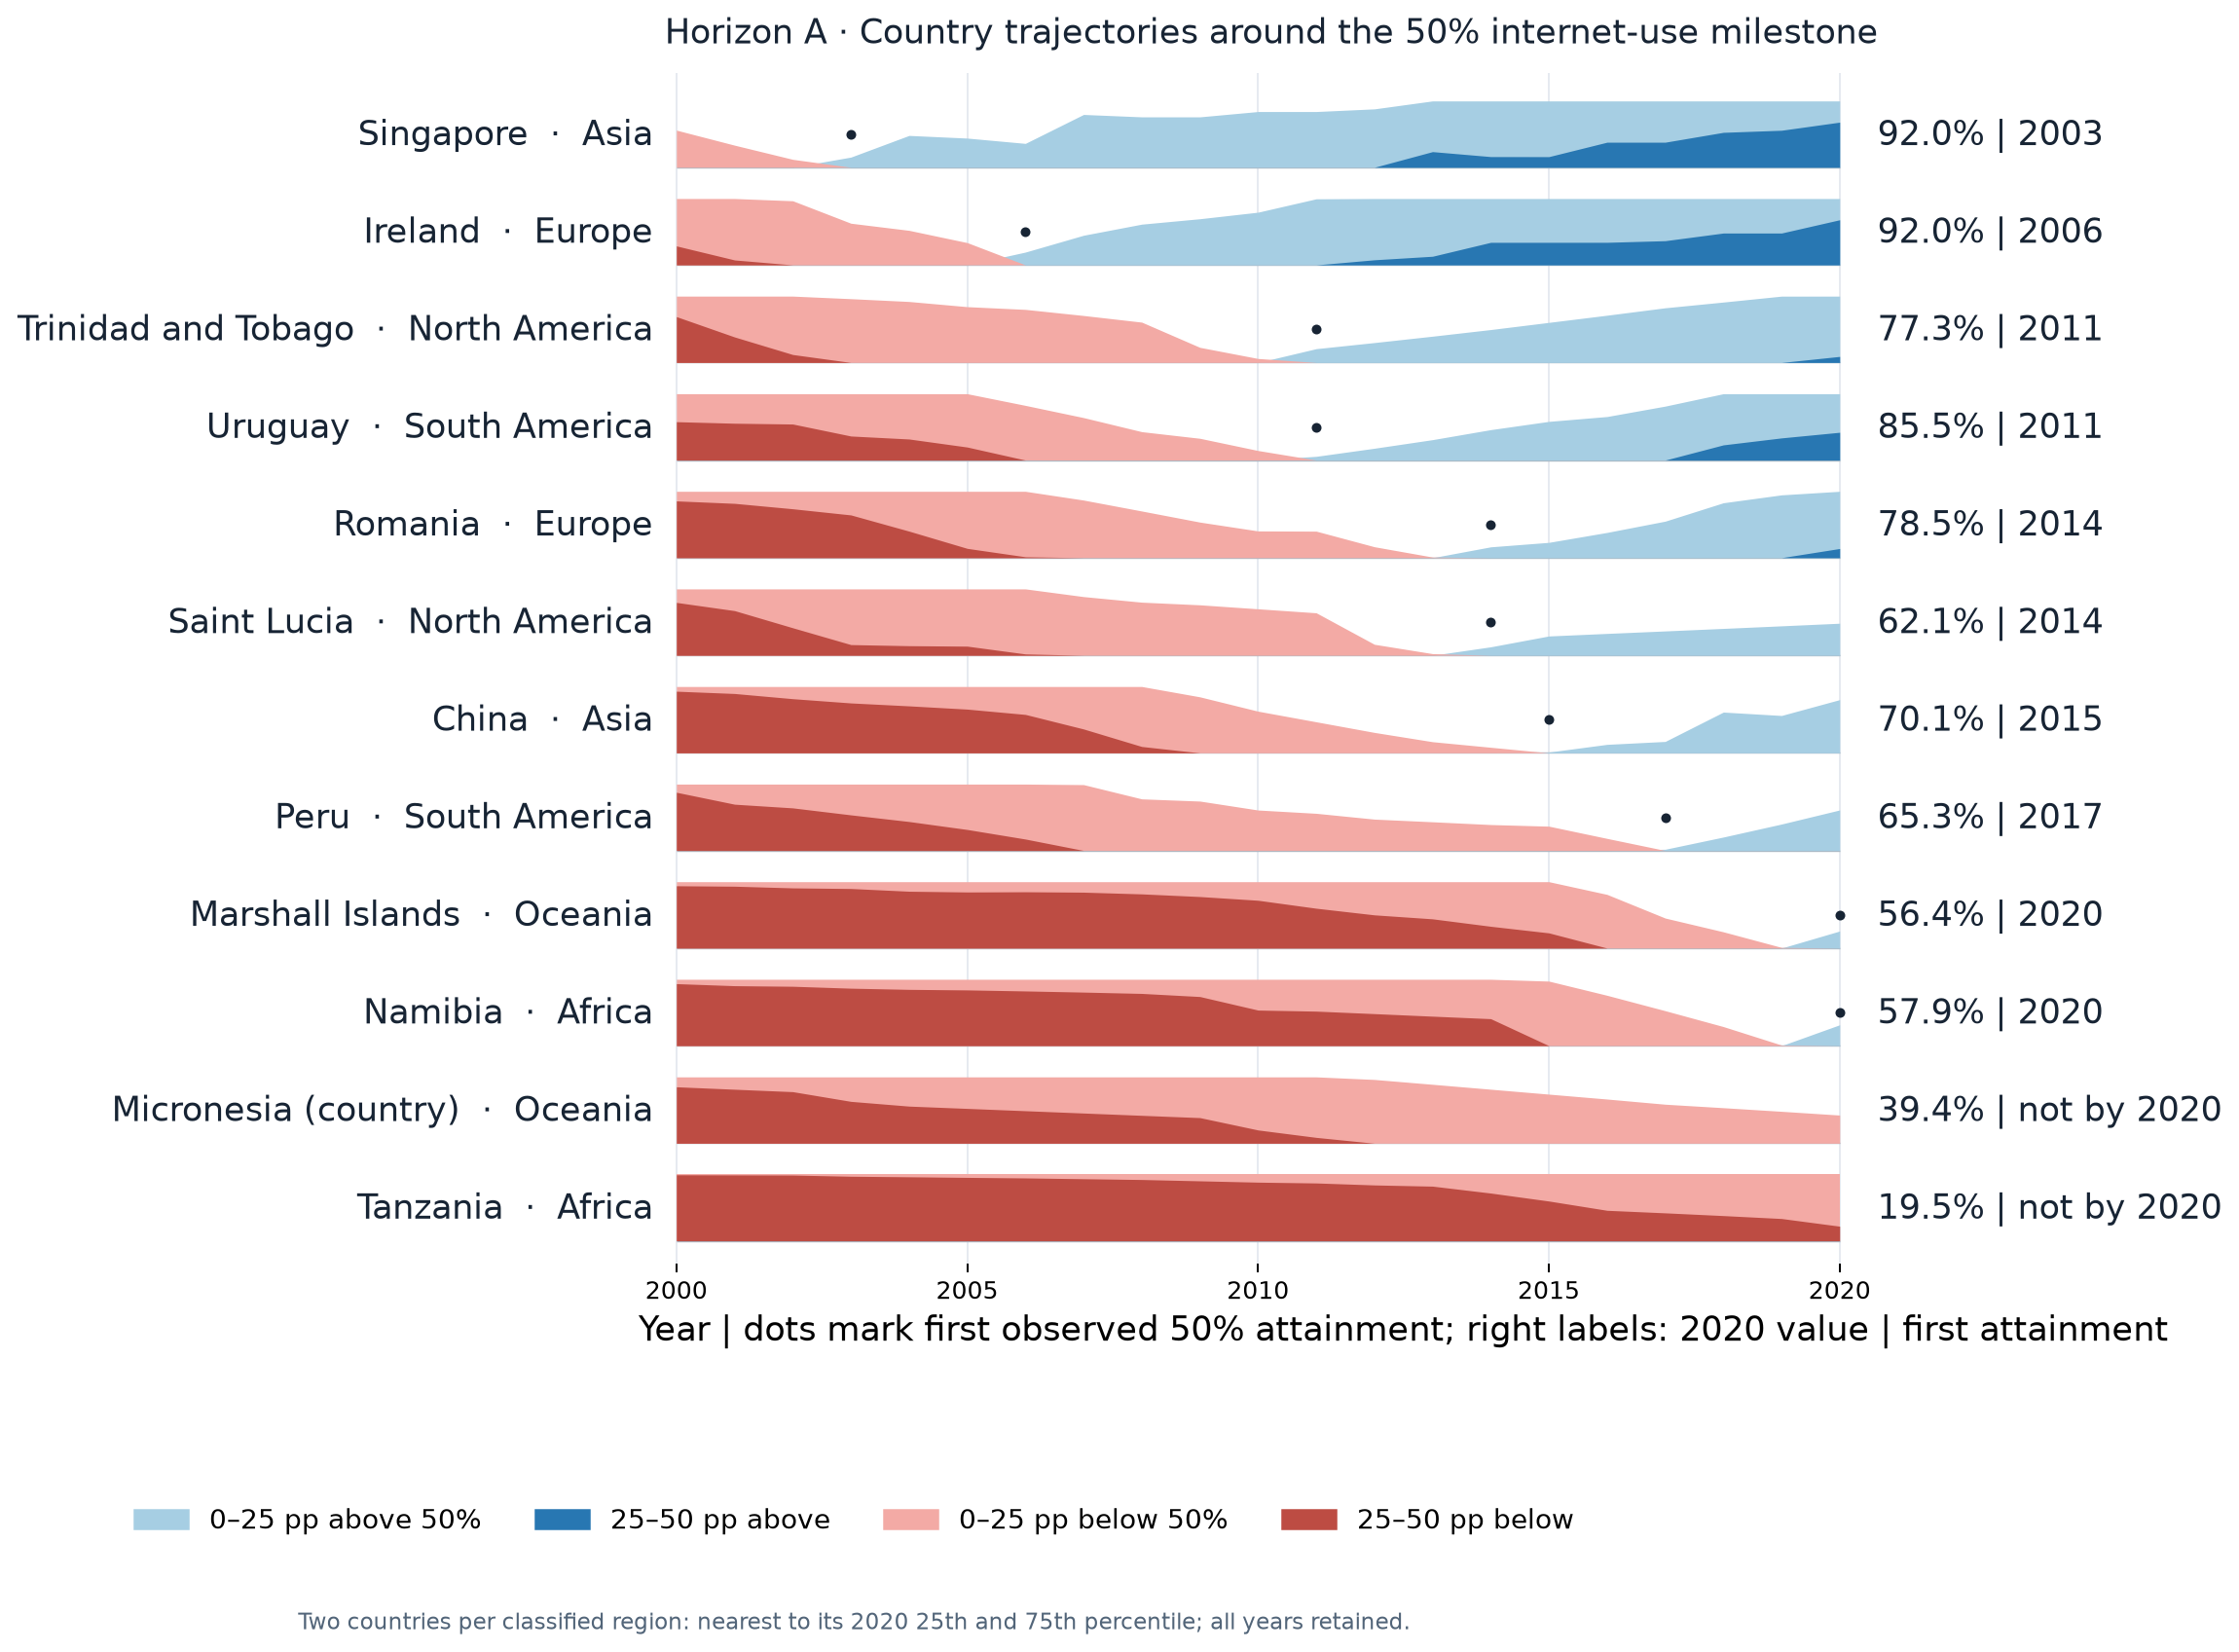
\includegraphics[width=\textwidth,height=0.49\textheight,keepaspectratio]{Fig14.png}

\caption{Country horizons reveal different majority-use crossing times. {\footnotesize \href{https://aithal007.github.io/DV_assignment2/figures.html\#fig14}{\textcolor{accent}{\underline{View figure and interpretation online}}}}}\label{fig:14}

\end{figure*}

\noindent\textit{How to read the graph.} Rows retain annual country adoption around a 50\% reference. Red/blue shows below/above; darkness folds 25-point bands. Dots mark first observed crossings.

\paragraph{Question.} Which countries reach majority internet use early or late?



\paragraph{Visual encoding.} Each row follows one selected country from 2000 to 2020. Red means below 50\% internet use and blue means above it. Darker bands mean a larger distance from 50\%. Right labels show the 2020 value and first observed 50\% year.



\paragraph{Why this visualization.} Many full-size time-series panels would take more space. Horizon rows fold values around a meaningful 50\% reference, keeping all 21 years in a compact display \cite{ref12}. Sorting by first crossing makes early and late arrivals easy to scan. The numerical endpoint labels help read values that are harder to recover from folded bands.



\paragraph{Interpretation.} The ordered rows show different first observed majority-use years: Singapore reaches 50\% in 2003, Ireland in 2006, China in 2015, Peru in 2017 and Namibia in 2020; Tanzania and Micronesia have no observed crossing by the endpoint. Those differences remain visible even where eventual adoption rates might look comparable.

Red/blue encodes position below/above the fixed 50\% reference; darkness distinguishes 25-point folded bands. A red row can still be rising rapidly. Annual sampling identifies the first recorded crossing year, not the precise date within that year. Two countries per classified region are selected by a stated endpoint-quartile rule. These examples recover timing hidden by a snapshot without pretending to represent every country or to measure growth directly from hue.



\paragraph{Scope and reading note.} Red means below the reference level, not falling internet use. A first crossing need not be permanent.



\takeaway{The same final adoption level can hide different arrival times. Horizon rows preserve early, late and absent crossings of the 50\% milestone. Their colors describe position relative to that reference; they do not by themselves indicate growth or decline.

}

\noindent\textit{Analytical recommendation.} Use first-crossing years to recover timing hidden by endpoints.

\subsection{Fig. 15: Regional median horizon plots}

\begin{figure*}[!tb]\centering

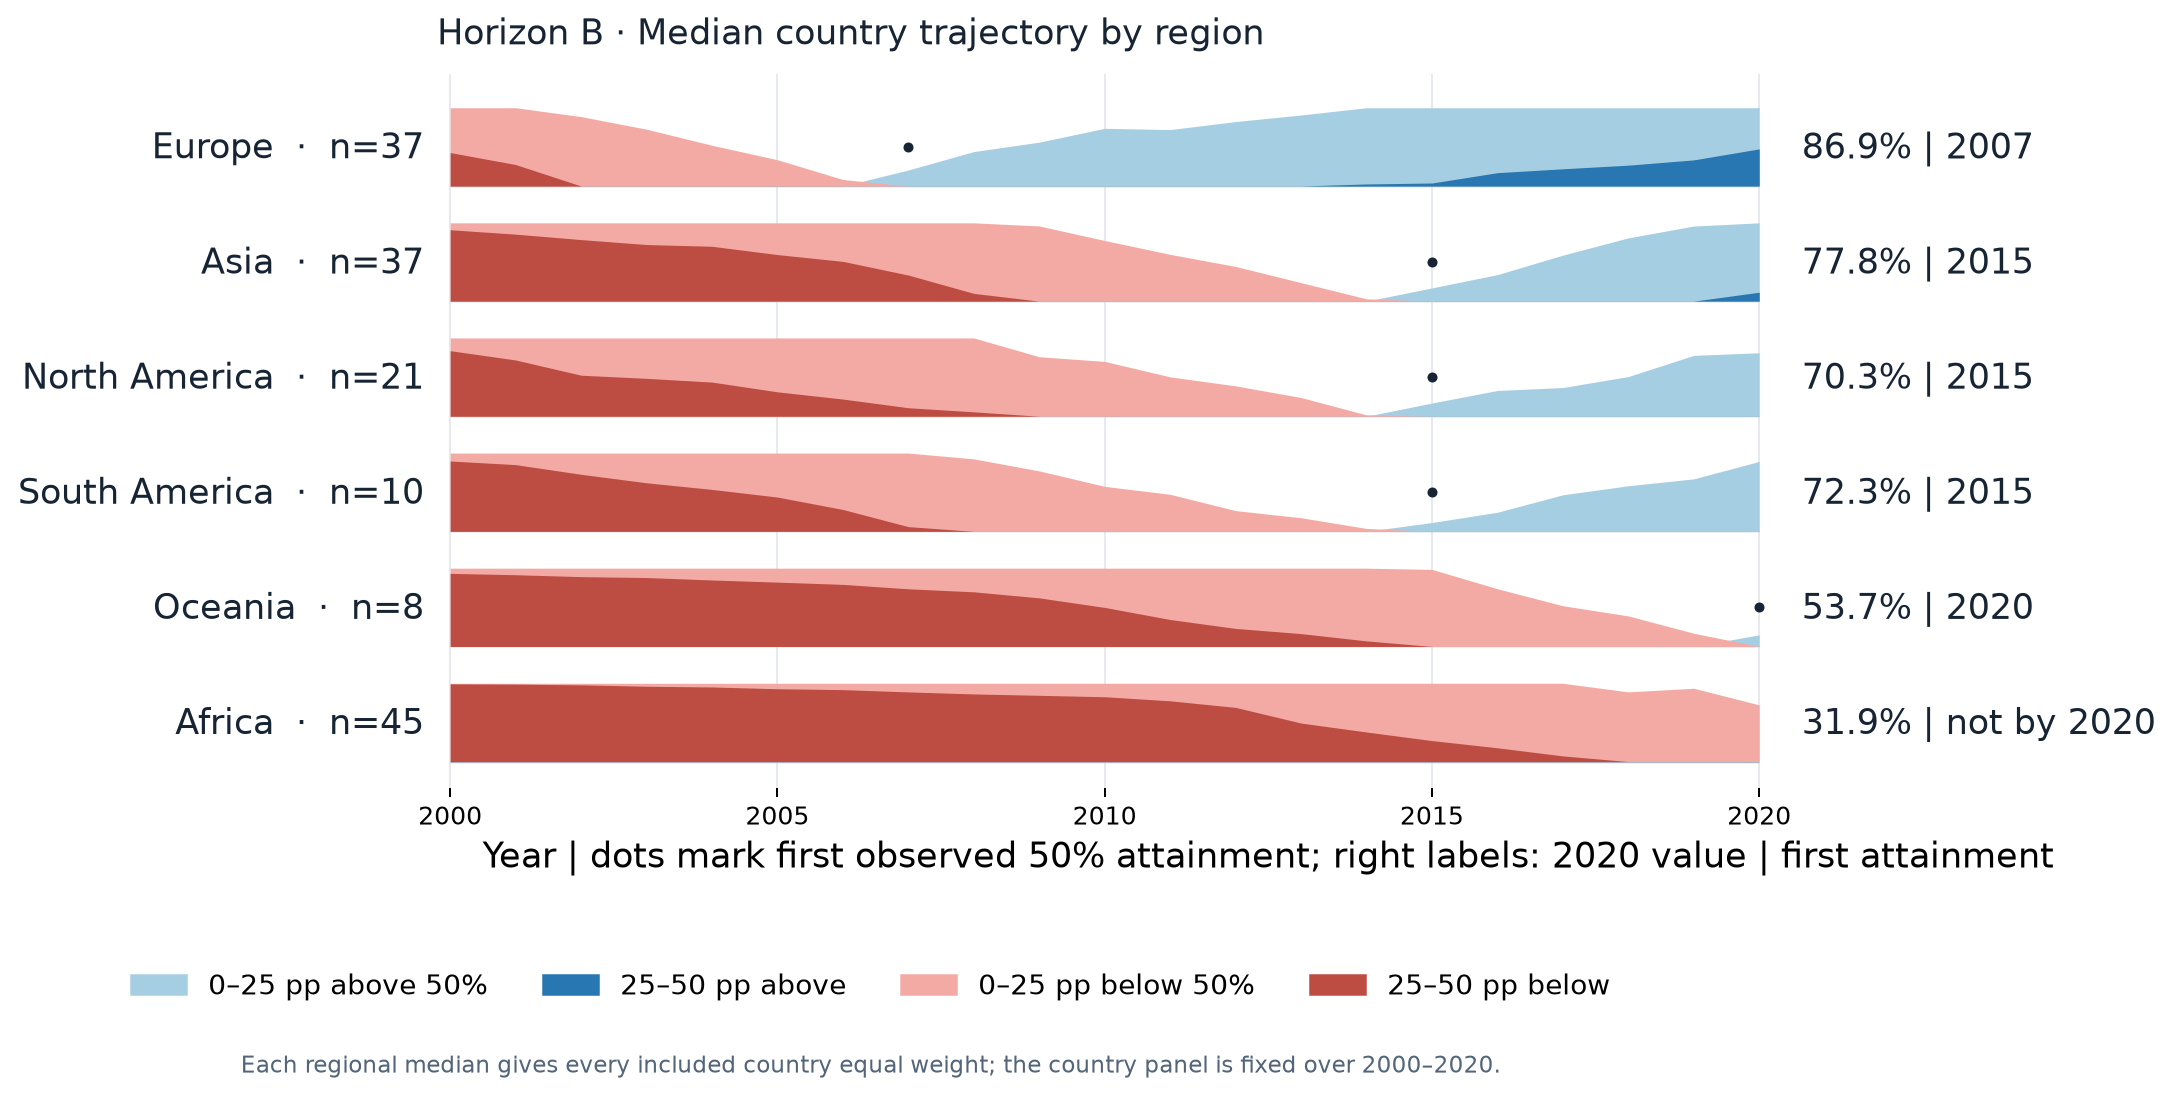
\includegraphics[width=\textwidth,height=0.34\textheight,keepaspectratio]{Fig15.png}

\caption{Regional trajectories differ; Oceania ends at 53.7\%. {\footnotesize \href{https://aithal007.github.io/DV_assignment2/figures.html\#fig15}{\textcolor{accent}{\underline{View figure and interpretation online}}}}}\label{fig:15}

\end{figure*}

\noindent\textit{How to read the graph.} Regional median histories use the same reference and bands. Right labels give 2020 adoption and first observed crossing; fixed regional memberships remain unchanged.

\paragraph{Question.} Do regional medians reach majority use at similar times?



\paragraph{Visual encoding.} Each row shows the yearly median internet-use rate for one region. The 50\% reference and band colors match Fig.~\ref{fig:14}. The same countries are used in every year.



\paragraph{Why this visualization.} Repeating the horizon design for regional medians tests how much the story changes after aggregation. The same reference and colors allow a direct comparison with Fig.~\ref{fig:14}. One compact row per region makes broad timing clear, while the preceding country plots show what each regional row leaves out.



\paragraph{Interpretation.} Europe's regional median ends at 86.86\%, Africa's at 31.89\%, and Oceania's at 53.71\% (53.7\% rounded, matching the 2020 median in Fig.~\ref{fig:17}). The fixed 50\% reference makes crossing time and endpoint level comparable; red means below majority access, not decline.

Each row is one regional median, so the roughly 55-point Europe-Africa endpoint gap compresses the variation among their countries. Fixed classified-country membership prevents changing coverage from creating the trajectories. Enlarging the regional horizon makes the endpoint labels readable; the regional ridgelines then recover the spread around each median.



\paragraph{Scope and reading note.} A regional median gives every included country equal weight; it does not describe every person in that region.



\takeaway{Regional trajectories make broad timing differences clear while compressing member histories. The large Europe-Africa median gap does not describe every country in either region. Read these summaries with country horizons and within-region spread before generalizing.

}

\noindent\textit{Analytical recommendation.} Compare regional trajectories, then inspect the country spread they compress.

\subsection{Fig. 16: How the country distribution changed}

\begin{figure*}[!tb]\centering

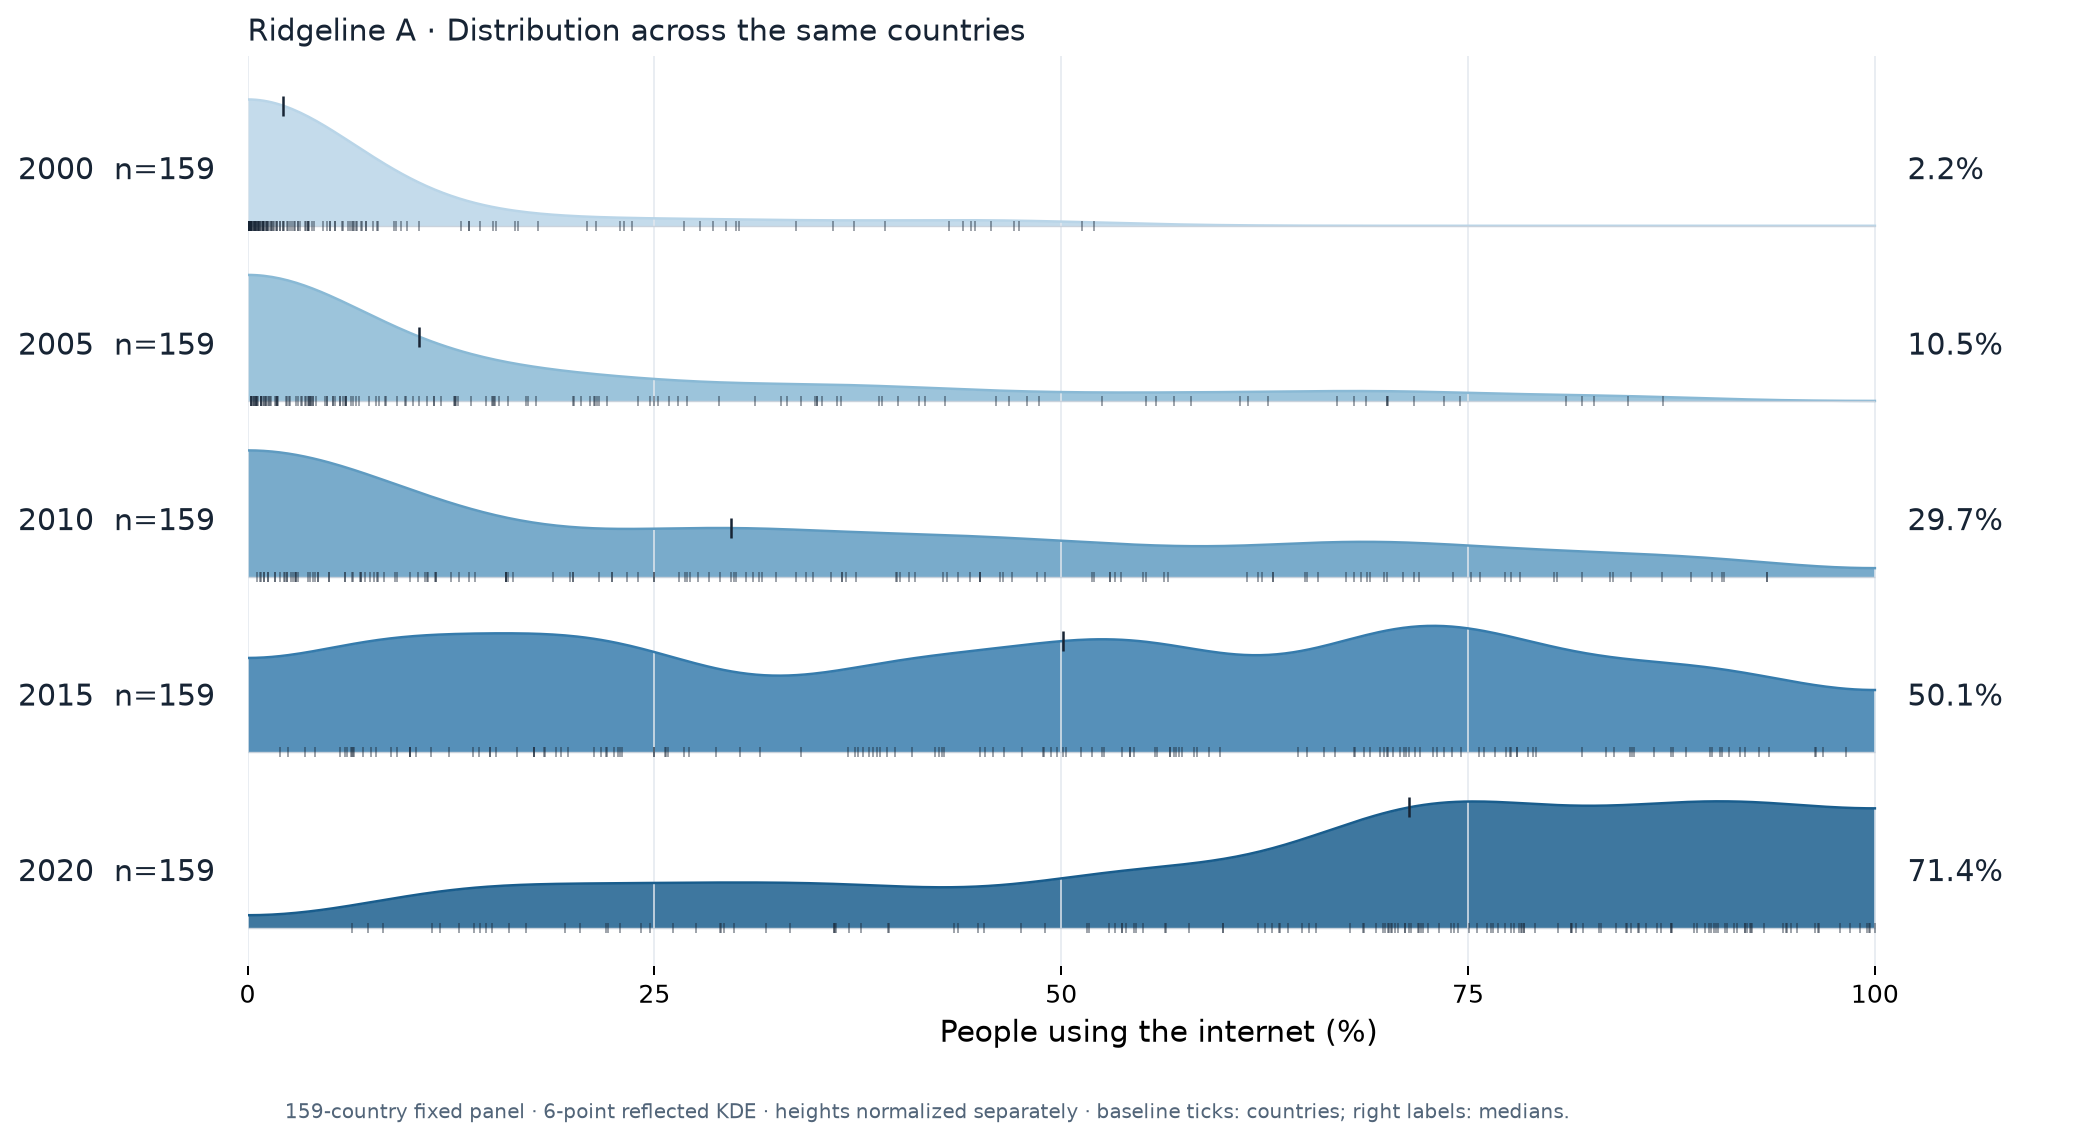
\includegraphics[width=\textwidth,height=0.35\textheight,keepaspectratio]{Fig16.png}

\caption{A rising median coexists with a broad 2020 distribution. {\footnotesize \href{https://aithal007.github.io/DV_assignment2/figures.html\#fig16}{\textcolor{accent}{\underline{View figure and interpretation online}}}}}\label{fig:16}

\end{figure*}

\noindent\textit{How to read the graph.} Ridges compare five yearly distributions of the same 159 countries on 0-100\%. Rugs retain observations and right labels medians; peak heights are normalized.

\paragraph{Question.} Did all countries move toward similar internet use?



\paragraph{Visual encoding.} Each ridge shows the distribution of internet use across the same 159 countries in one year. All ridges share the 0-100\% scale. Small ticks show countries, and right labels give the median.



\paragraph{Why this visualization.} A rising median could mean that countries moved together or that some moved much faster than others. Ridgelines retain the whole distribution at several dates. A common horizontal scale shows the shift, while country ticks help check the smooth shapes against the actual observations.



\paragraph{Interpretation.} The ridges shift right as the country median rises from 2.2\% in 2000 to 71.4\% in 2020. Yet the 2020 middle half still spans about 37.5 percentage points. The horizontal width and country ticks show that broad progress has not produced a narrow common adoption level.

All five distributions use the same 159 countries and the same 0-100\% axis, so the comparison is not driven by membership changes. Ridge heights are independently normalized; a taller peak does not mean more countries. Smoothing estimates shape between observations, whereas the ticks retain actual values. This supports the main question directly: a much larger median can coexist with substantial remaining dispersion. The fixed-cohort plot is needed for the separate question of who caught up.



\paragraph{Scope and reading note.} Curves use a reflected Gaussian density with a six-percentage-point bandwidth. Each ridge is scaled separately for shape.



\takeaway{A rising country median does not mean adoption has become uniform. Despite the rise from 2.2\% to 71.4\%, the 2020 middle half spans 37.5 points. Distribution width qualifies the progress visible in the central value.

}

\noindent\textit{Analytical recommendation.} Read distribution width alongside the rise in the median.

\subsection{Fig. 17: How distributions changed within regions}

\begin{figure*}[!tb]\centering

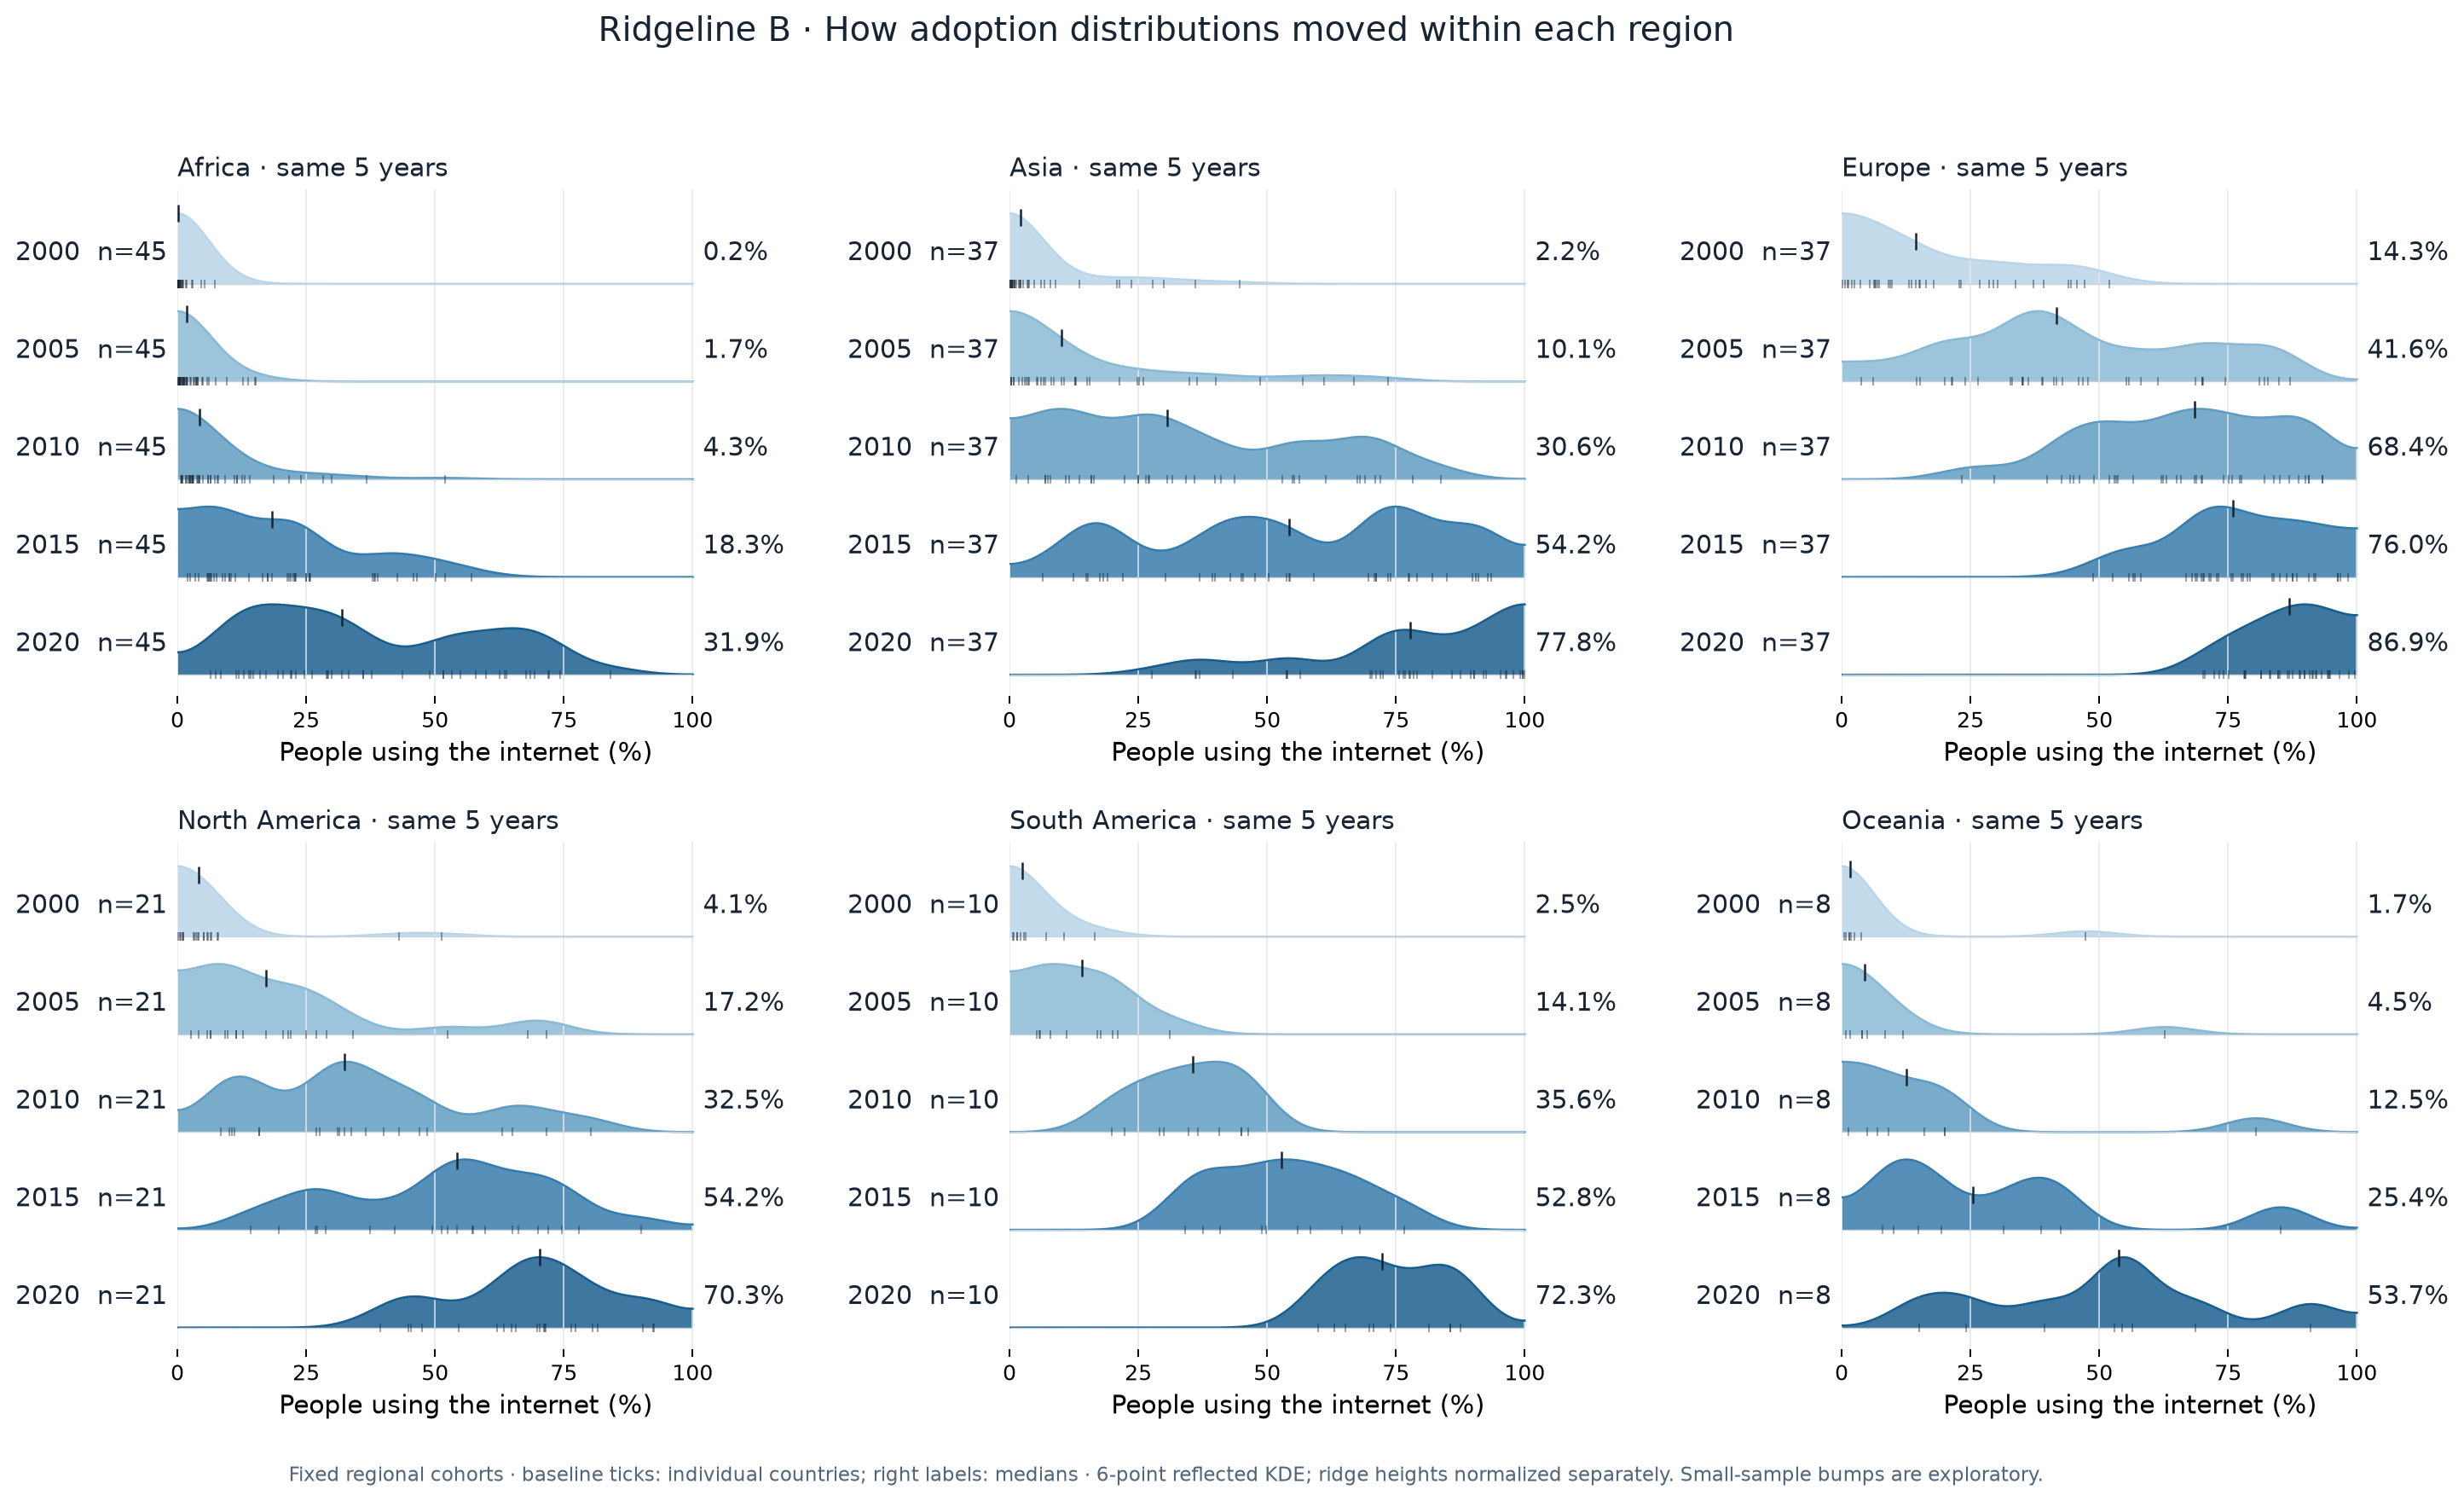
\includegraphics[width=\textwidth,height=0.49\textheight,keepaspectratio]{Fig17.png}

\caption{Regional distribution histories differ behind the global shift. {\footnotesize \href{https://aithal007.github.io/DV_assignment2/figures.html\#fig17}{\textcolor{accent}{\underline{View figure and interpretation online}}}}}\label{fig:17}

\end{figure*}

\noindent\textit{How to read the graph.} Six regional panels repeat the five-year ridgeline comparison with fixed memberships. Shared horizontal scales support timing and spread comparisons; rug marks retain countries.

\paragraph{Question.} Which regional differences are hidden by the whole-panel distribution?



\paragraph{Visual encoding.} Each panel repeats the ridgeline view within one region for 2000, 2005, 2010, 2015 and 2020. All panels use the same internet-use scale. Country ticks and median labels help check the smooth curves.



\paragraph{Why this visualization.} The global distribution mixes countries from different regions. Small multiples repeat the ridgeline comparison within each region, so a broad global shape can be traced to different regional paths. Shared horizontal scales keep low and high adoption in the same position across all panels.



\paragraph{Interpretation.} Europe's ridges move toward high adoption earlier, while later African ridges still occupy low and middle values. Asia's distributions remain broad during its movement to the right. These distinct positions and widths explain how the global progress pattern combines different regional histories rather than one common shift.

The shared horizontal scale and unchanged country membership support temporal comparison inside each region. The small Oceania sample contains only eight included countries (Cohort C, n=159), making its individual ticks more reliable evidence than a smooth bump alone. Note that Fig.~\ref{fig:13} uses the broader Cohort B (n=175) for regional endpoint comparisons; the Oceania 2015 median in this ridgeline (Cohort C, 159 countries) therefore need not equal the value implied by Fig.~\ref{fig:13}'s different cohort. Peak height is normalized within each ridge and should not be compared as a population count. These panels recover both between-region timing and internal spread that a single regional median horizon compresses.



\paragraph{Scope and reading note.} Small groups can produce bumps that are not stable patterns. Curve height is not a country count. Rounded labels can also coincide: Asia and North America both print 54.2\% for 2015, while their exact medians differ slightly (54.22\% versus 54.21\%).



\takeaway{Global progress combines different regional histories and changing internal spreads. A single global ridge therefore cannot represent one shared journey. Country marks are essential when small groups make a smooth density shape look more certain than the observations support.

}

\noindent\textit{Analytical recommendation.} Inspect regional histories before treating global progress as a shared trajectory.

\FloatBarrier

\section{Scalar fields and visual encodings}

Controlled experiments hold measured weather fields fixed while varying palette, temporal normalization and contour representation.



\subsection{Fig. 18: How color choices change the view}

\begin{figure*}[!tb]\centering

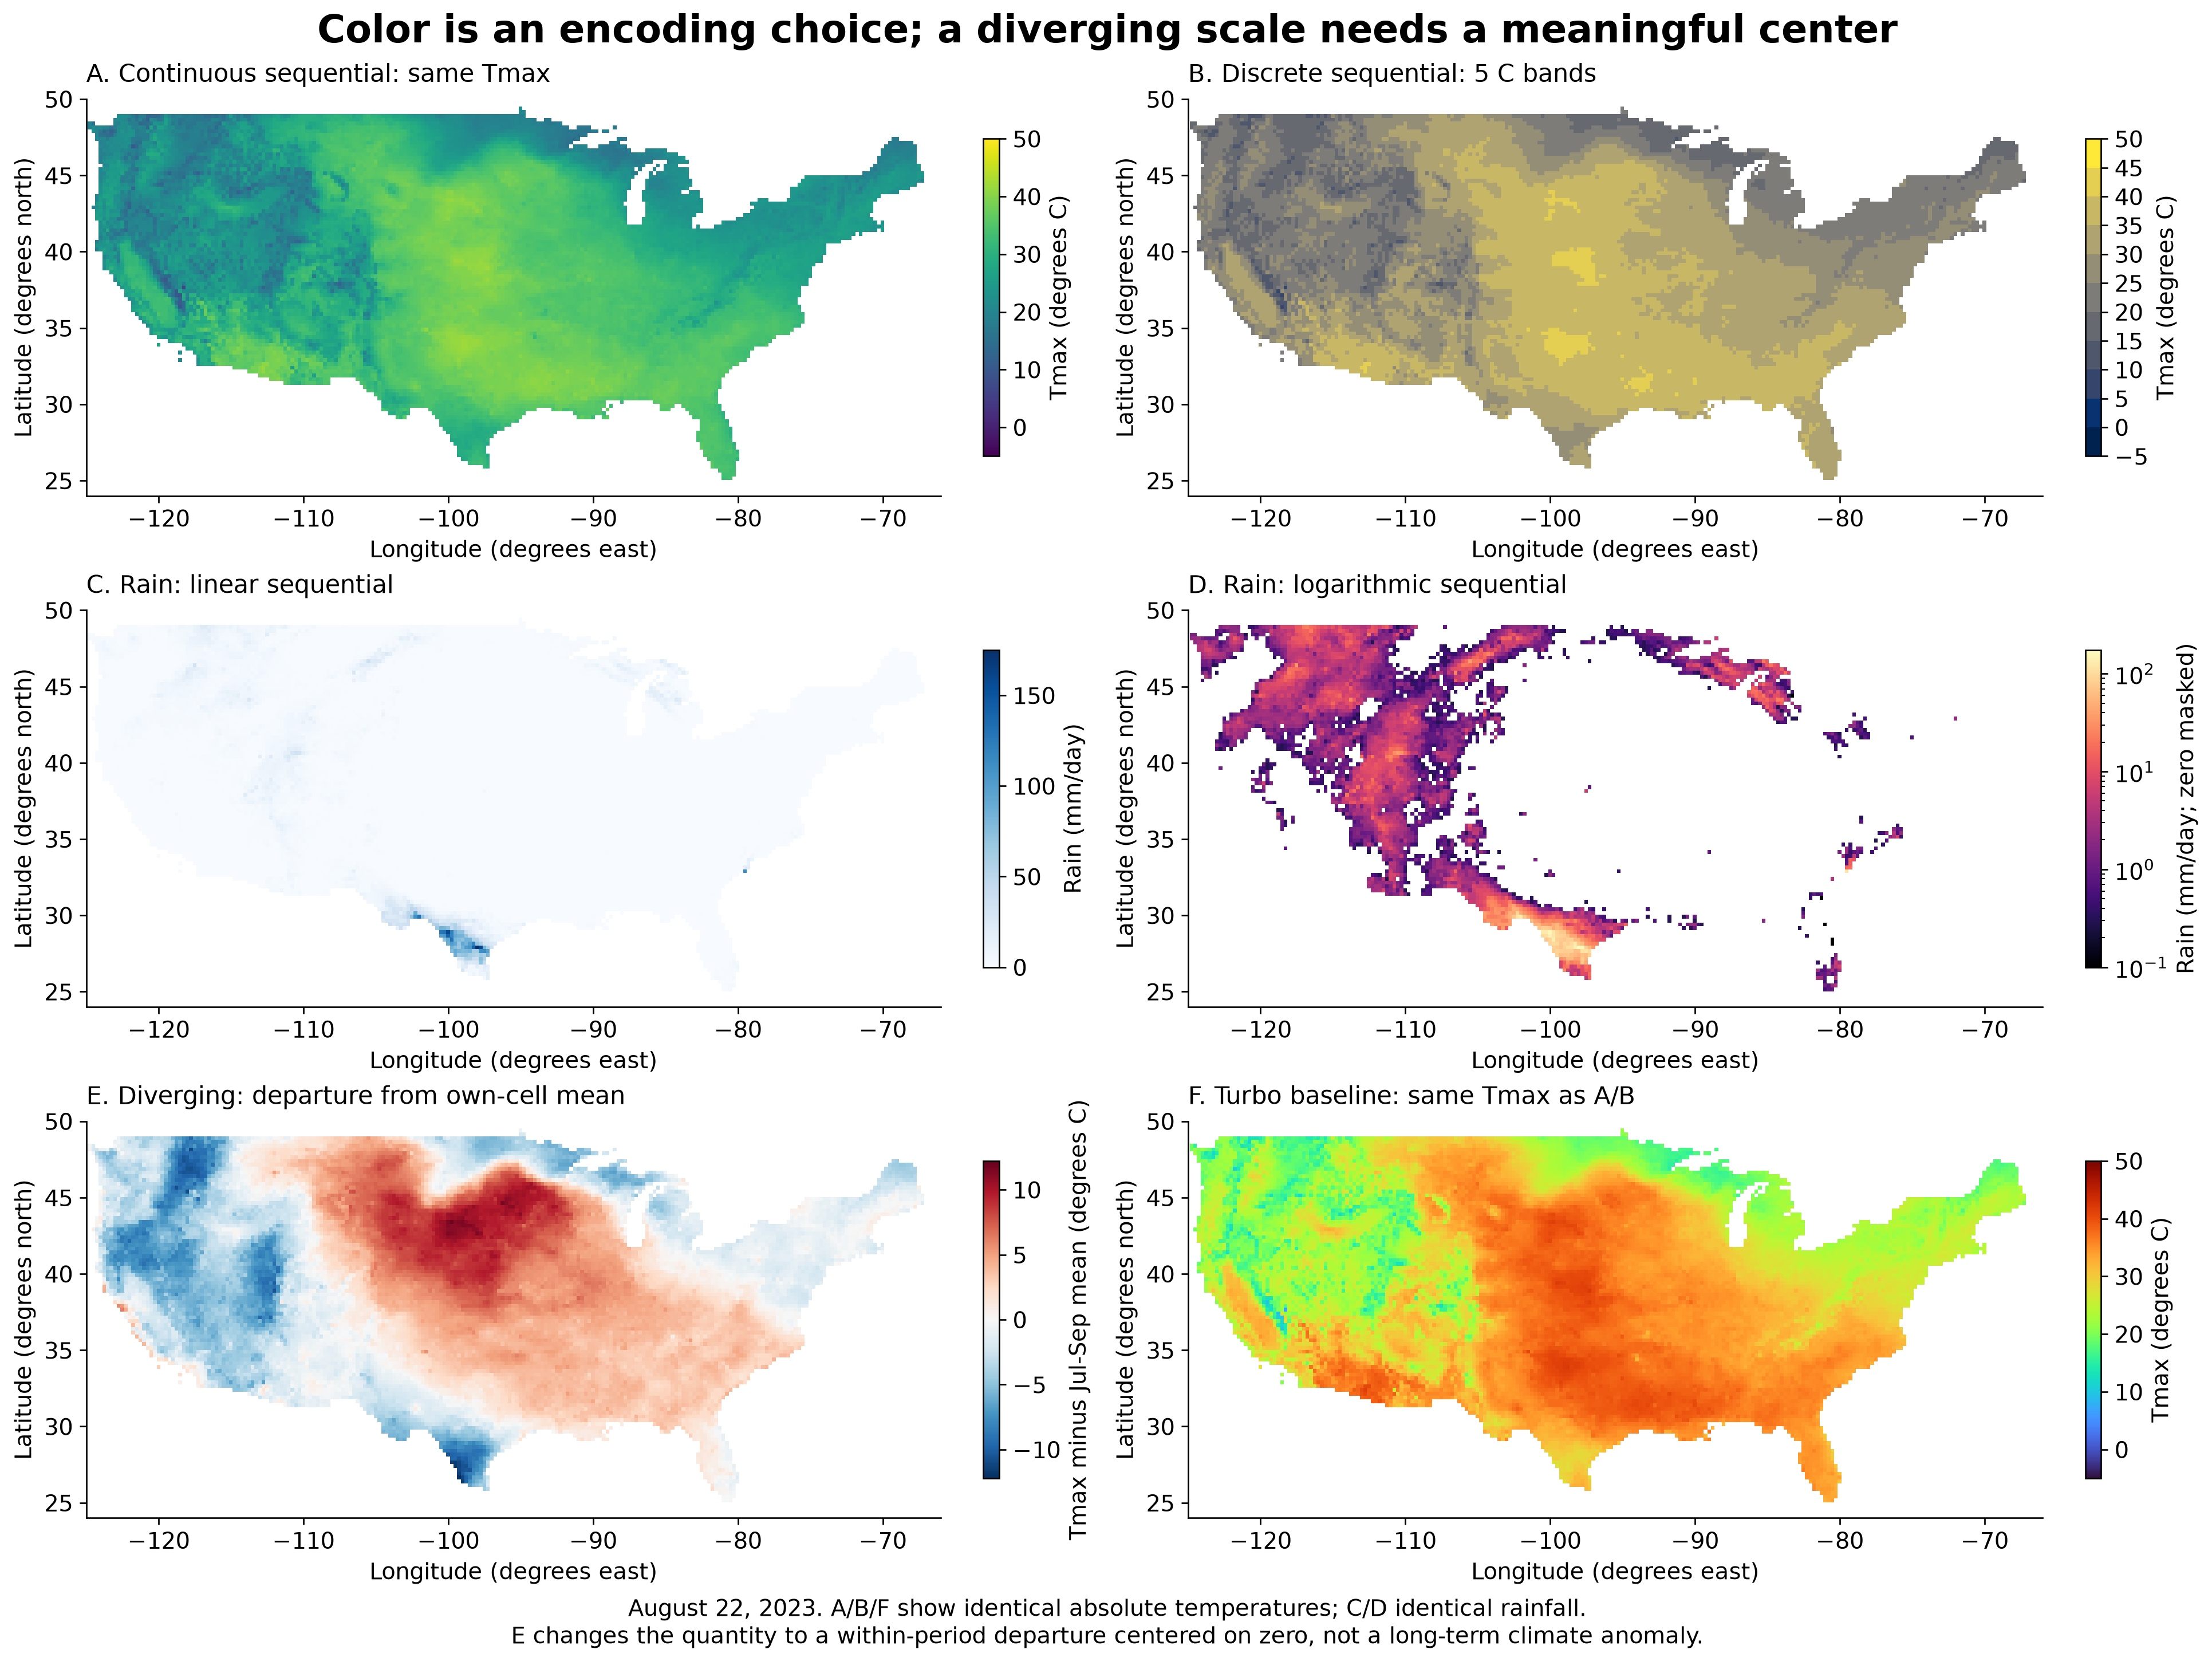
\includegraphics[width=\textwidth,height=0.62\textheight,keepaspectratio]{Fig18.png}

\caption{Identical values change appearance; zero-centered departures require a different encoding. {\footnotesize \href{https://aithal007.github.io/DV_assignment2/figures.html\#fig18}{\textcolor{accent}{\underline{View figure and interpretation online}}}}}\label{fig:18}

\end{figure*}

\noindent\textit{How to read the graph.} A/B/F hold absolute Tmax fixed; C/D hold rainfall fixed. E changes to a zero-centered within-period temperature departure, requiring a diverging scale.

\paragraph{Question.} What changes when the same field uses a different color mapping?



\paragraph{Visual encoding.} The panels keep the weather field and date fixed. Panels A-D use sequential palettes whose colors progress from lower to higher values: temperature uses continuous viridis (A) and cividis split into 5-degree bands (B), and rain uses Blues with a linear scale (C) and magma with a logarithmic scale (D). Panel E needs a diverging scale because departures from a local mean extend in both directions, and panel F keeps turbo as a deliberately poor baseline. Palette choice and scale normalization are separate choices. Read each color bar before comparing the maps.



\paragraph{Why this visualization.} A palette or scale can make a feature stand out even when the measurements do not change. These panels hold the field fixed and change only its mapping to color. Sequential colormaps suit these ordered magnitudes because no middle value needs special emphasis. Temperature tests palette choice; rainfall tests how the scale reveals smaller values alongside heavy rain.



\paragraph{Interpretation.} Panels A, B, and F display absolute daily maximum temperature on August 22: continuous viridis, 5-degree discrete cividis steps with an authentic stepped colorbar, and the unsegmented turbo baseline \cite{ref15}. Panels C and D compare linear and logarithmic rainfall with zero rain masked in white. Sequential palettes suit ordered physical magnitudes \cite{ref7}; the turbo baseline demonstrates the perceptual banding and ordering hazards documented by Borland and Taylor \cite{ref15}.

Panel E deliberately changes the quantity to each cell's daily Tmax minus its own July-September mean. Zero separates warmer and cooler departures, justifying symmetric diverging RdBu\_r. Keeping the quantity and normalization explicit prevents reading palette-induced contrast as additional physical structure; turbo hues have no extra measurement meaning.



\paragraph{Scope and reading note.} Zero rain is masked for logarithmic mapping. Color contrast by itself is not a change in the data.



\takeaway{Color mapping controls which measured differences receive visual emphasis. Linear rain color prioritizes absolute amounts, while logarithmic color separates small positive amounts. Interpret a feature through its legend and normalization before calling it a stronger weather event.

}

\noindent\textit{Analytical recommendation.} Choose a color center only when it has a meaningful data reference.

\subsection{Fig. 19: Fixed and daily color scales}

\begin{figure*}[!tb]\centering

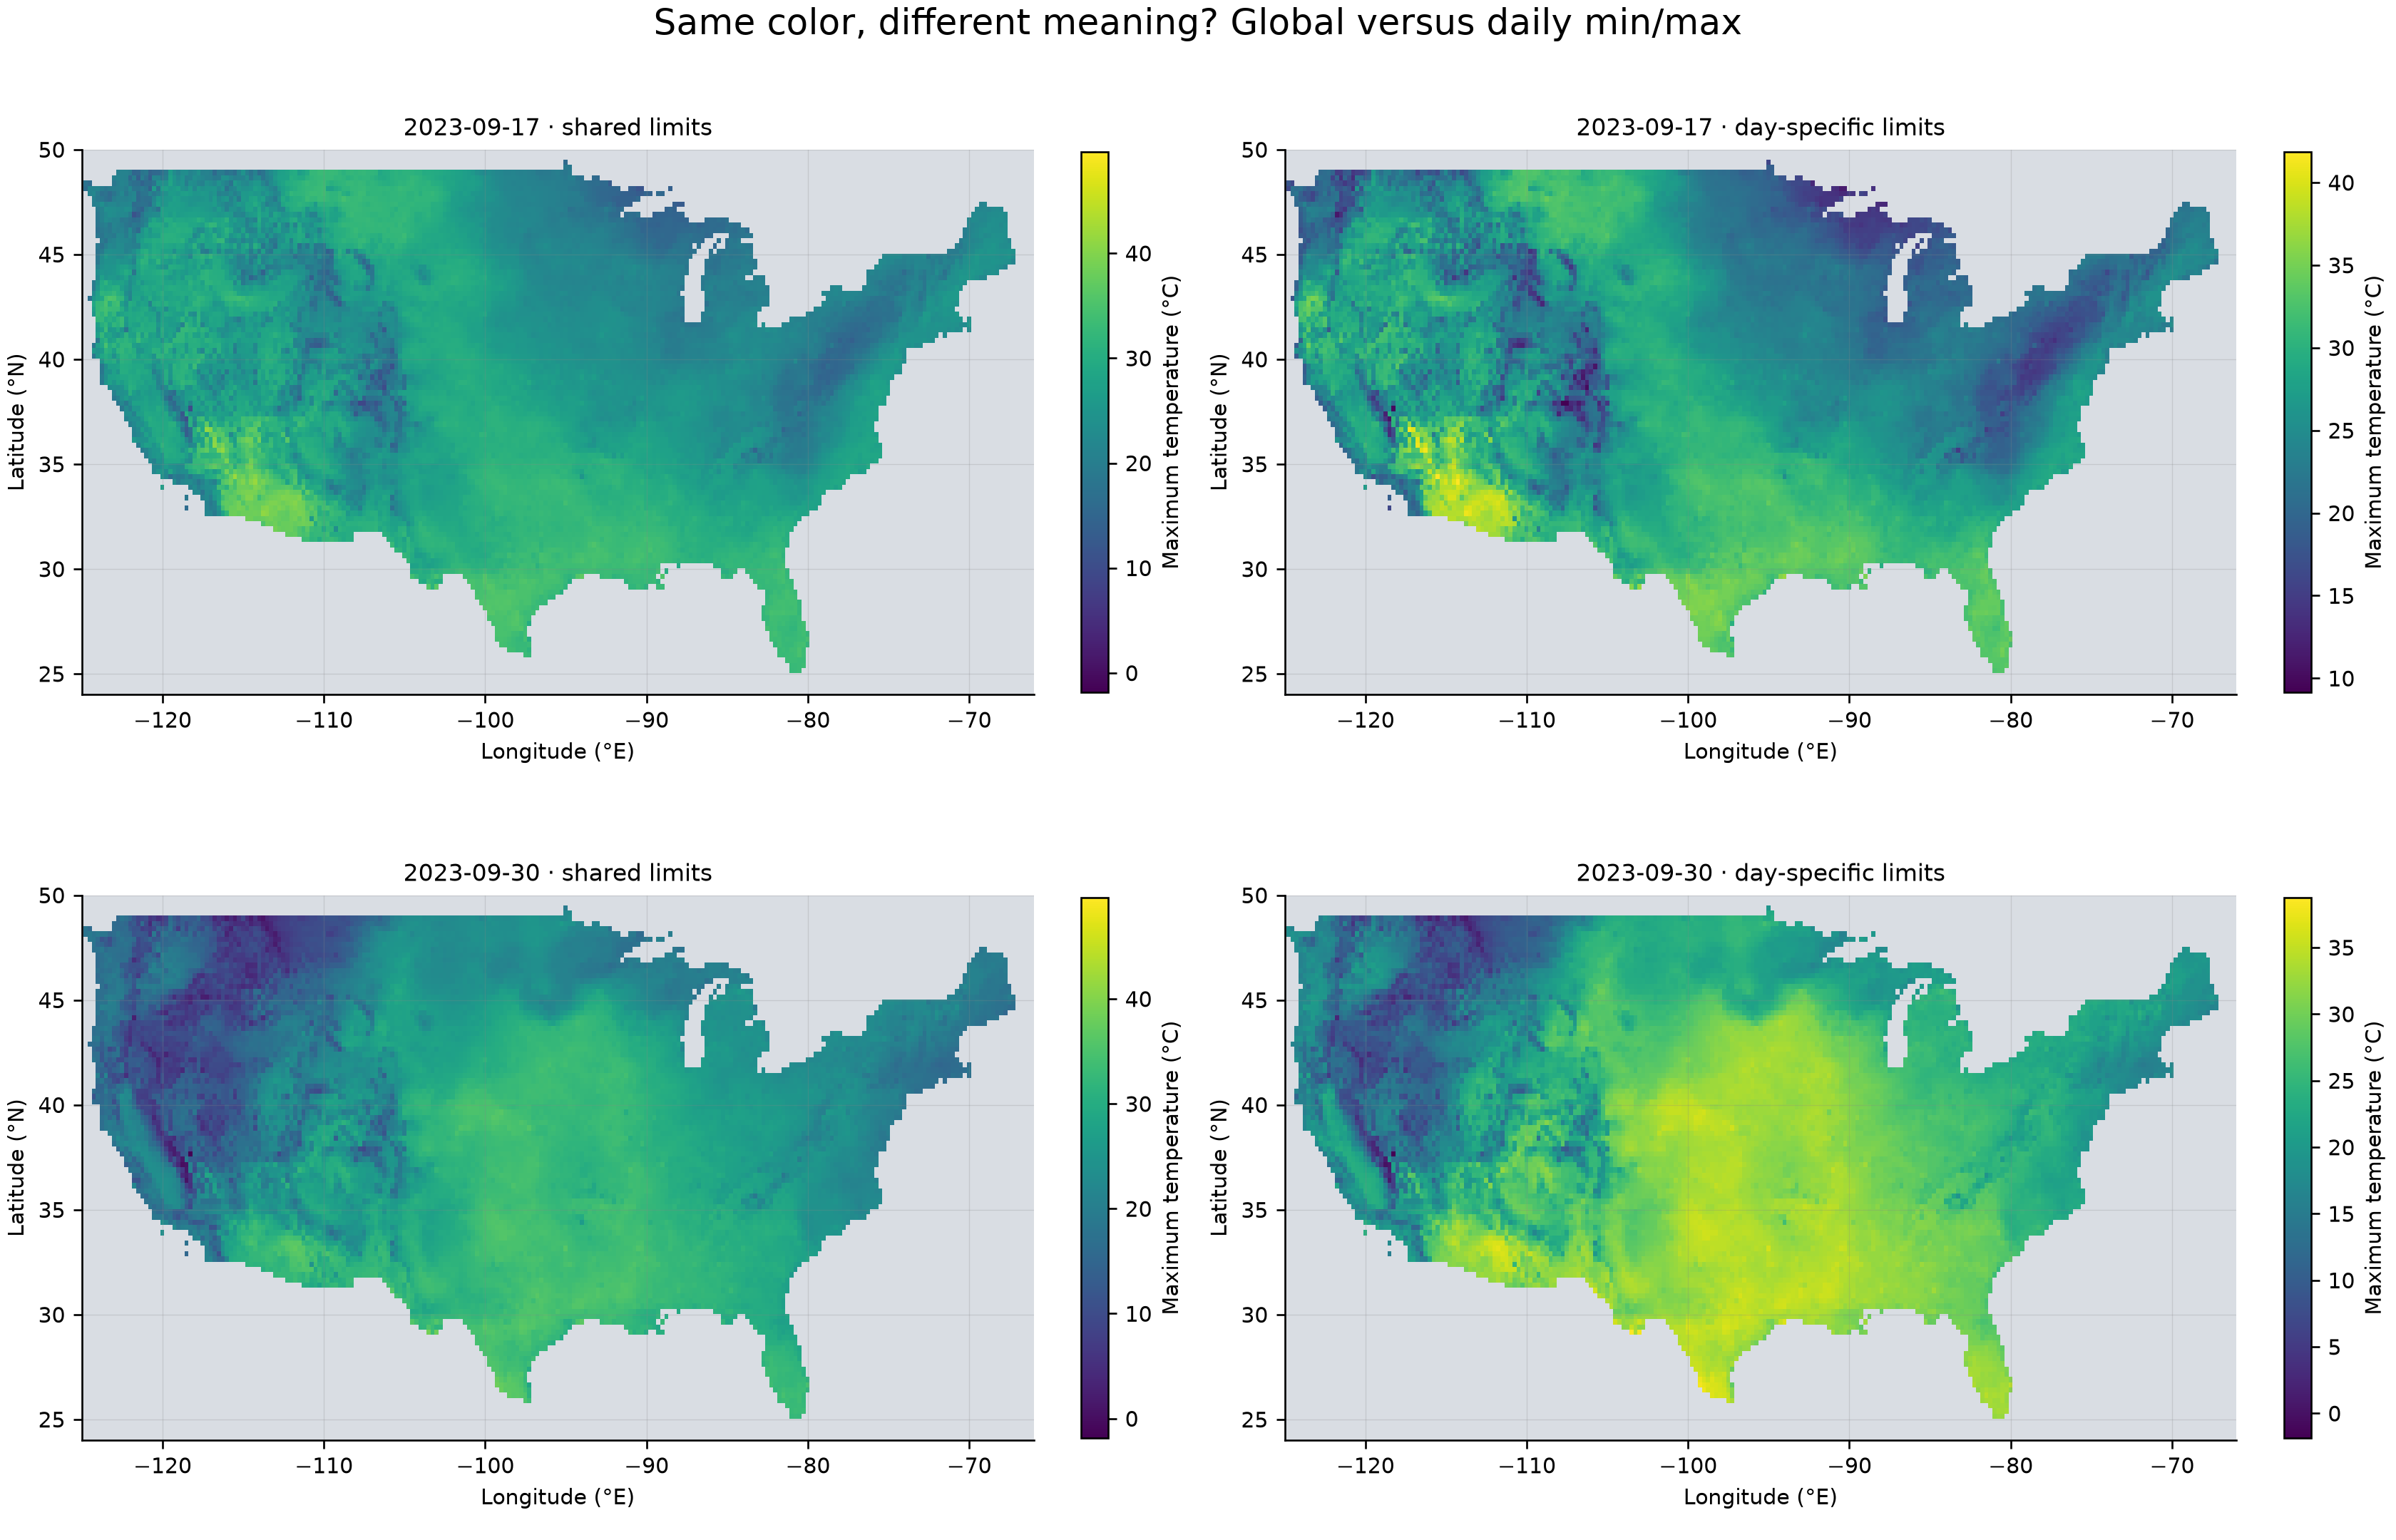
\includegraphics[width=\textwidth,height=0.49\textheight,keepaspectratio]{Fig19.png}

\caption{Daily rescaling changes the numerical meaning of the same color. {\footnotesize \href{https://aithal007.github.io/DV_assignment2/images/scivis/scivis_global.gif}{\textcolor{accent}{\underline{View fixed-scale animation}}} \quad | \quad \href{https://aithal007.github.io/DV_assignment2/images/scivis/scivis_local.gif}{\textcolor{accent}{\underline{View daily-scale animation}}}}}\label{fig:19}

\end{figure*}

\noindent\textit{How to read the graph.} Identical temperature fields use fixed eight-date extrema at left and each date's extrema at right. Read the separate colorbars before comparing colors.

\paragraph{Question.} Can the same color mean a different temperature?



\paragraph{Visual encoding.} The left column uses one temperature range across the eight sampled dates. The right column rescales each date to its own minimum and maximum. Both columns show the same fields.



\paragraph{Why this visualization.} An animation can look equally warm on every date if each frame is rescaled separately. The two columns test this with identical daily fields. One scale preserves comparisons between dates; the other spends its full color range on the variation within each date. Neither choice can be understood without checking the color bars.



\paragraph{Interpretation.} The paired columns map identical daily fields using two parameter rules. Global normalization uses u=(T-min)/(max-min) with bounds fixed over the eight frames; daily normalization recomputes those bounds for each date. Consequently, the same warm hue may mark different temperatures in the daily column even when both frames use their full palette.

The fixed eight-date range is -1.85 to 49.65 C. It supports between-frame comparison without claiming to cover extremes on every unsampled day. Daily scaling is useful for within-date contrasts but cannot support reading repeated color as repeated absolute temperature. The GIFs make this issue explicit over time. This explains a visual inference failure that can occur before any statistical aggregation: inconsistent encodings can conceal the change the animation is meant to reveal.



\paragraph{Scope and reading note.} The fixed limits come from the eight samples, not from all 92 days or a long-term climate record.



\takeaway{Consistent colors are necessary for comparing temperature across dates. Daily rescaling can assign the same bright color to different temperatures, concealing absolute change. Use fixed bounds for temporal comparison and daily bounds for within-date contrast.

}

\noindent\textit{Analytical recommendation.} Use fixed scales to compare dates; use local scales to inspect within-date detail.

\subsection{Fig. 20: Contour intervals and filled contours}

\begin{figure*}[!tb]\centering

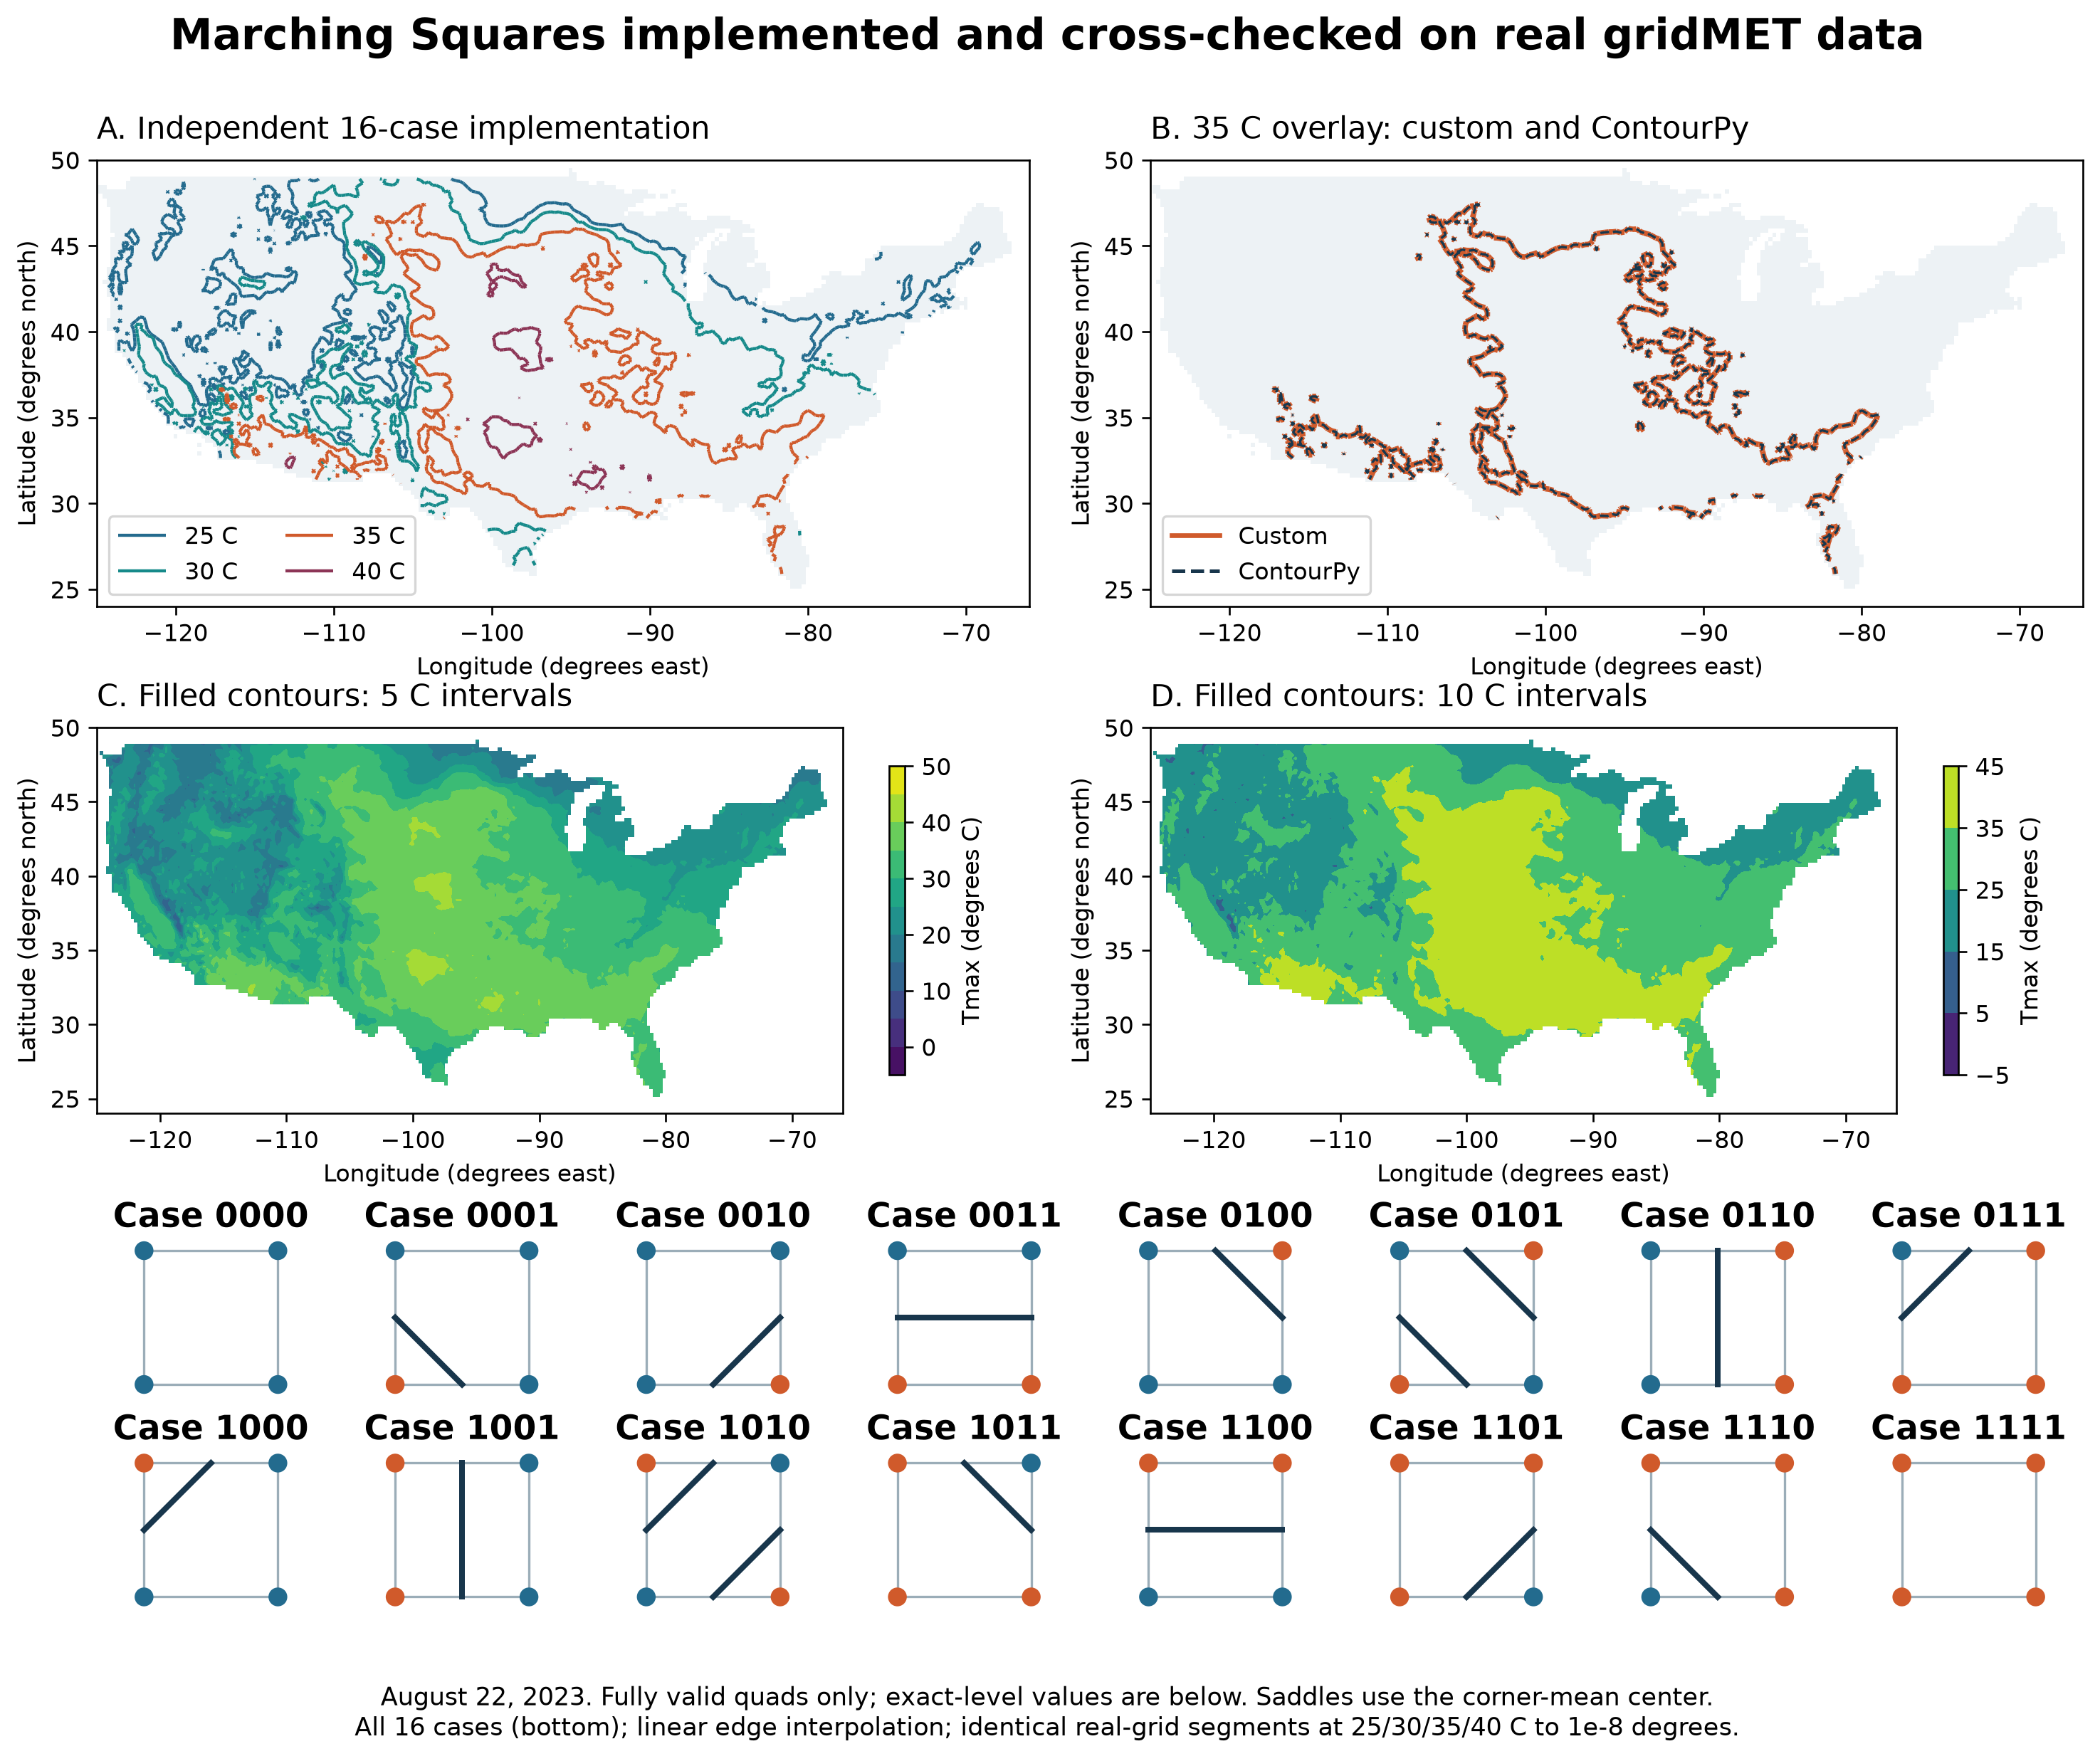
\includegraphics[width=\textwidth,height=0.68\textheight,keepaspectratio]{Fig20.png}

\caption{Custom lines match ContourPy at four thresholds; filled bands trade boundary detail for regional readability. {\footnotesize \href{https://aithal007.github.io/DV_assignment2/images/scivis/scivis_contour.gif}{\textcolor{accent}{\underline{View contour animation}}}}}\label{fig:20}

\end{figure*}

\noindent\textit{How to read the graph.} A: custom 16-case tracing. B: 35 C overlay against ContourPy. C/D: five-/ten-degree filled bands. Bottom diagrams show the corner configurations.

\paragraph{Question.} How much boundary detail does the contour interval show?



\paragraph{Visual encoding.} A: independent line tracing. B: custom/ContourPy 35 C overlay. C/D: five-/ten-degree filled bands. Bottom: all 16 corner cases; orange corners are above threshold. The same fully valid quads and linear interpolation support the comparison.



\paragraph{Why this visualization.} Contours turn a continuous field into visible boundaries. Using the same date with two intervals separates the effect of boundary spacing from actual weather differences. Lines make threshold crossings explicit, while filled bands make broad areas easier to compare. The four panels test both choices on the same grid.



\paragraph{Interpretation.} An independent 16-case Marching Squares algorithm generates the contour topology: four corner bits classify each fully valid quad; linear interpolation locates edge crossings; saddle cases are resolved using the corner-mean center. Exact-level values count as below. The bottom diagrams expose all 16 cases, including ambiguous topological configurations \cite{ref6,ref14} (ref14 describes the 3D Marching Cubes; the 2D Marching Squares topology used here is the direct 2D analogue of the same case-table principle).

The custom lines match ContourPy serial at 25, 30, 35 and 40 C to 1e-8 degrees on the actual August 22 grid; 32 synthetic case/center checks confirm exact boundary closure. Custom line tracing provides exact threshold verification, while ContourPy filled bands delineate regional thermal zones. Five- versus ten-degree bands change display detail, not source resolution.



\paragraph{Scope and reading note.} More contour lines mean more displayed detail, not more observations or a changed field.



\takeaway{More contour lines increase display detail without increasing data resolution. Five-degree spacing reveals more threshold crossings; filled bands emphasize broad regions. Select the representation for the reading task and infer boundaries only at the stated levels.

}

\noindent\textit{Analytical recommendation.} Use traced thresholds for boundaries and filled bands for regional comparison.

\section{Weather across complete months and days}

We restore all 92 dates to compare cooling, rainfall concentration, repeated heat and episode timing.



\subsection{Fig. 21: Monthly temperature maps}

\begin{figure*}[!tb]\centering

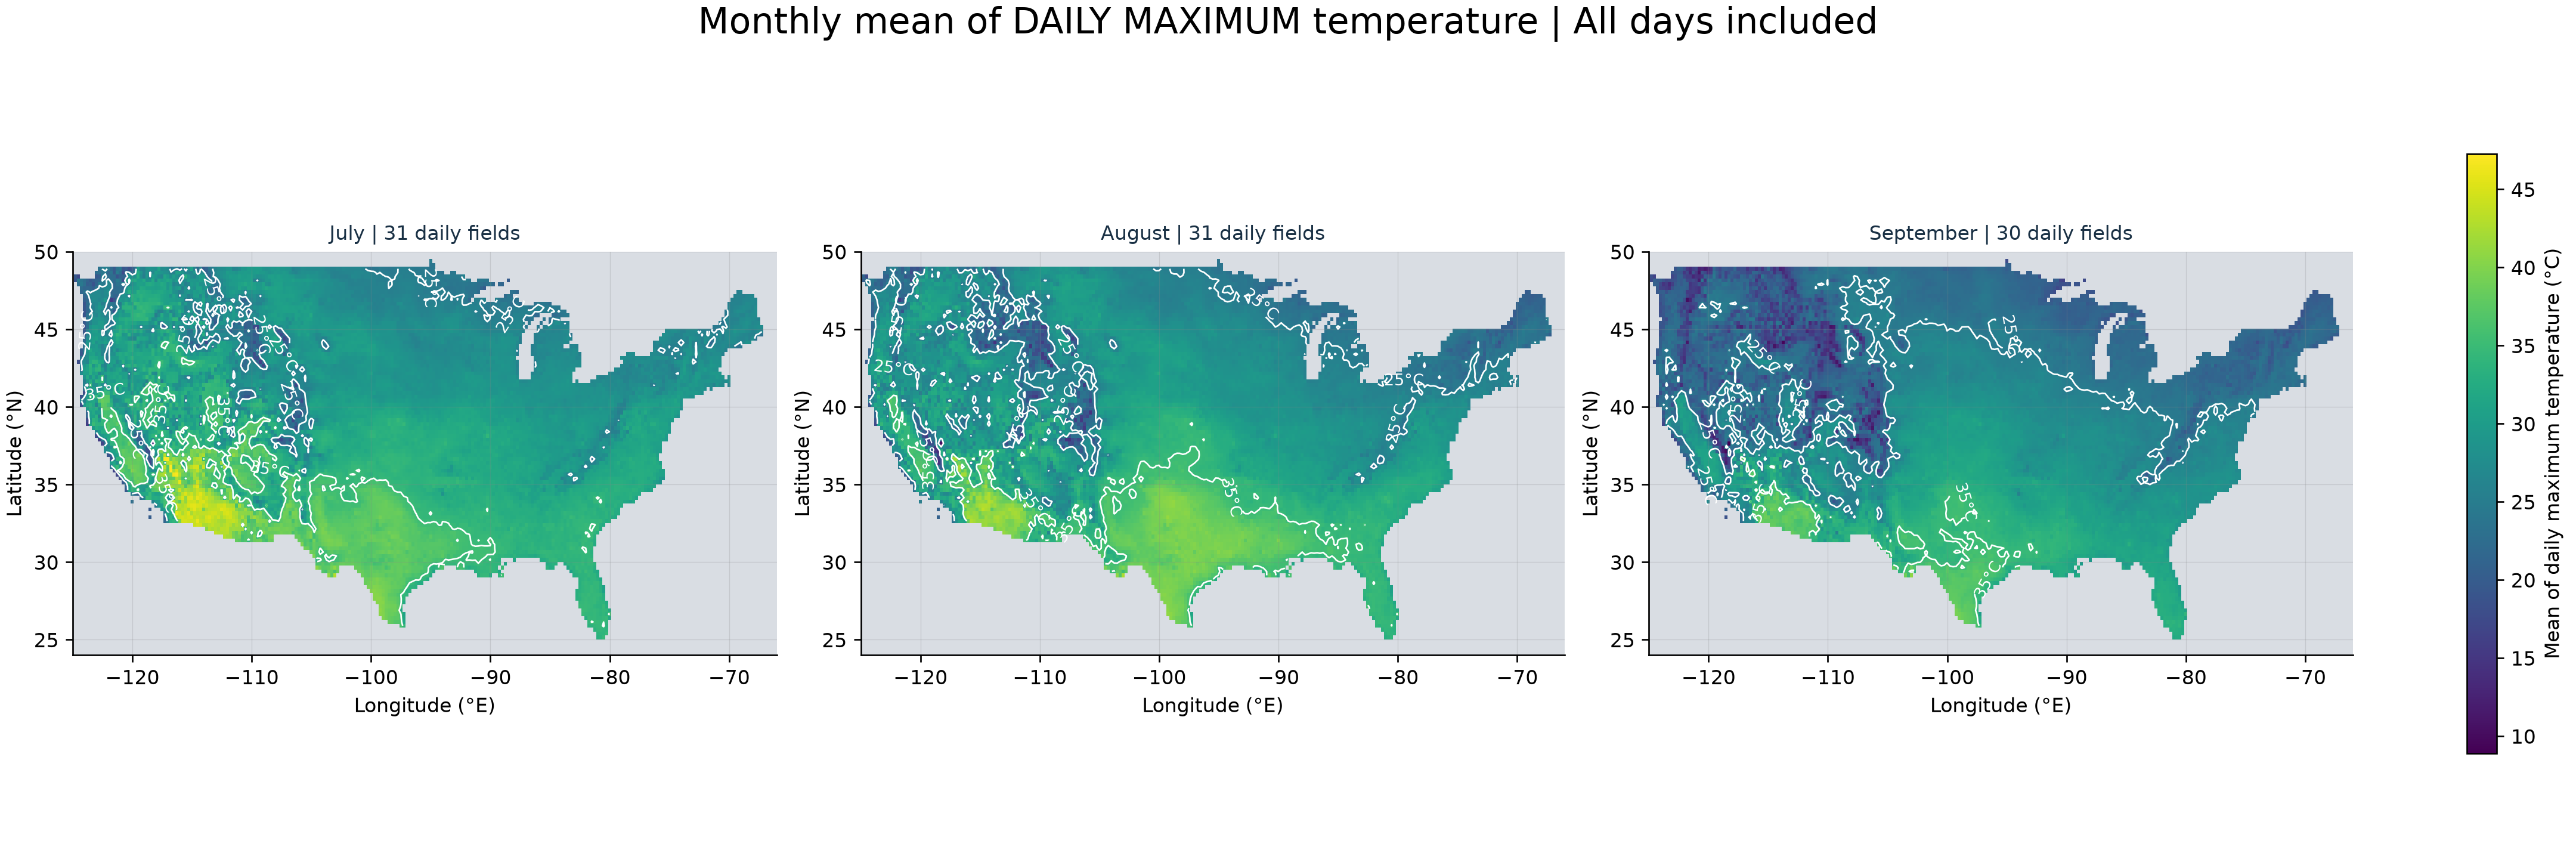
\includegraphics[width=\textwidth,height=0.49\textheight,keepaspectratio]{Fig21.png}

\caption{Complete-month means cool while retaining geographic differences. {\footnotesize \href{https://aithal007.github.io/DV_assignment2/figures.html\#fig21}{\textcolor{accent}{\underline{View figure and interpretation online}}}}}\label{fig:21}

\end{figure*}

\noindent\textit{How to read the graph.} Three monthly maps average all daily maxima on the common footprint. Background color encodes temperature ($^{\circ}$C); contour lines provide explicit isothermal reference boundaries: dashed lines delineate the 25\textdegree{}C isotherm and solid lines delineate the 35\textdegree{}C isotherm.

\paragraph{Question.} How does the average daily maximum temperature change across the three months?



\paragraph{Visual encoding.} Each map averages daily maximum temperature over one month. All maps use the same Celsius scale and the same reference contour levels: the 25\textdegree{}C contour marks the transition from mild to warm regions, and the 35\textdegree{}C contour isolates persistent high-heat cores.



\paragraph{Why this visualization.} After testing color and contours, we use fixed choices to compare complete months. Shared colors let a temperature be recognized across all three maps, and common contour levels give reference boundaries. Using every day avoids choosing one unusually hot or cool date to represent a month.



\paragraph{Interpretation.} The same color and 25/35 C contours make monthly temperatures comparable. Mean daily maximum temperature falls from 31.19 C in July to 26.55 C in September over the weighted common footprint, while southern warm areas remain visible. The maps establish both the broad decline and its nonuniform spatial pattern.

Each month uses every daily maximum, so one unusually hot or cool day is not made its representative. The mapped quantity is an average of daily maxima, not a monthly extreme or an average of hourly temperatures. Monthly averaging still removes short spells and the order of days. The following difference map tests the spatial extent of cooling, and daily/frequency views recover the event information needed to interpret that seasonal summary.



\paragraph{Scope and reading note.} These are monthly averages of daily maxima, not monthly extremes or averages of every hourly temperature.



\takeaway{The monthly maps establish broad cooling while retaining its spatial pattern. The mean daily maximum falls by 4.64 degrees, but a monthly average cannot count heat episodes or their duration. Daily and frequency views supply those missing dimensions.

}

\noindent\textit{Analytical recommendation.} Follow monthly means with daily views to recover timing.

\subsection{Fig. 22: Monthly change versus two selected dates}

\begin{figure*}[!tb]\centering

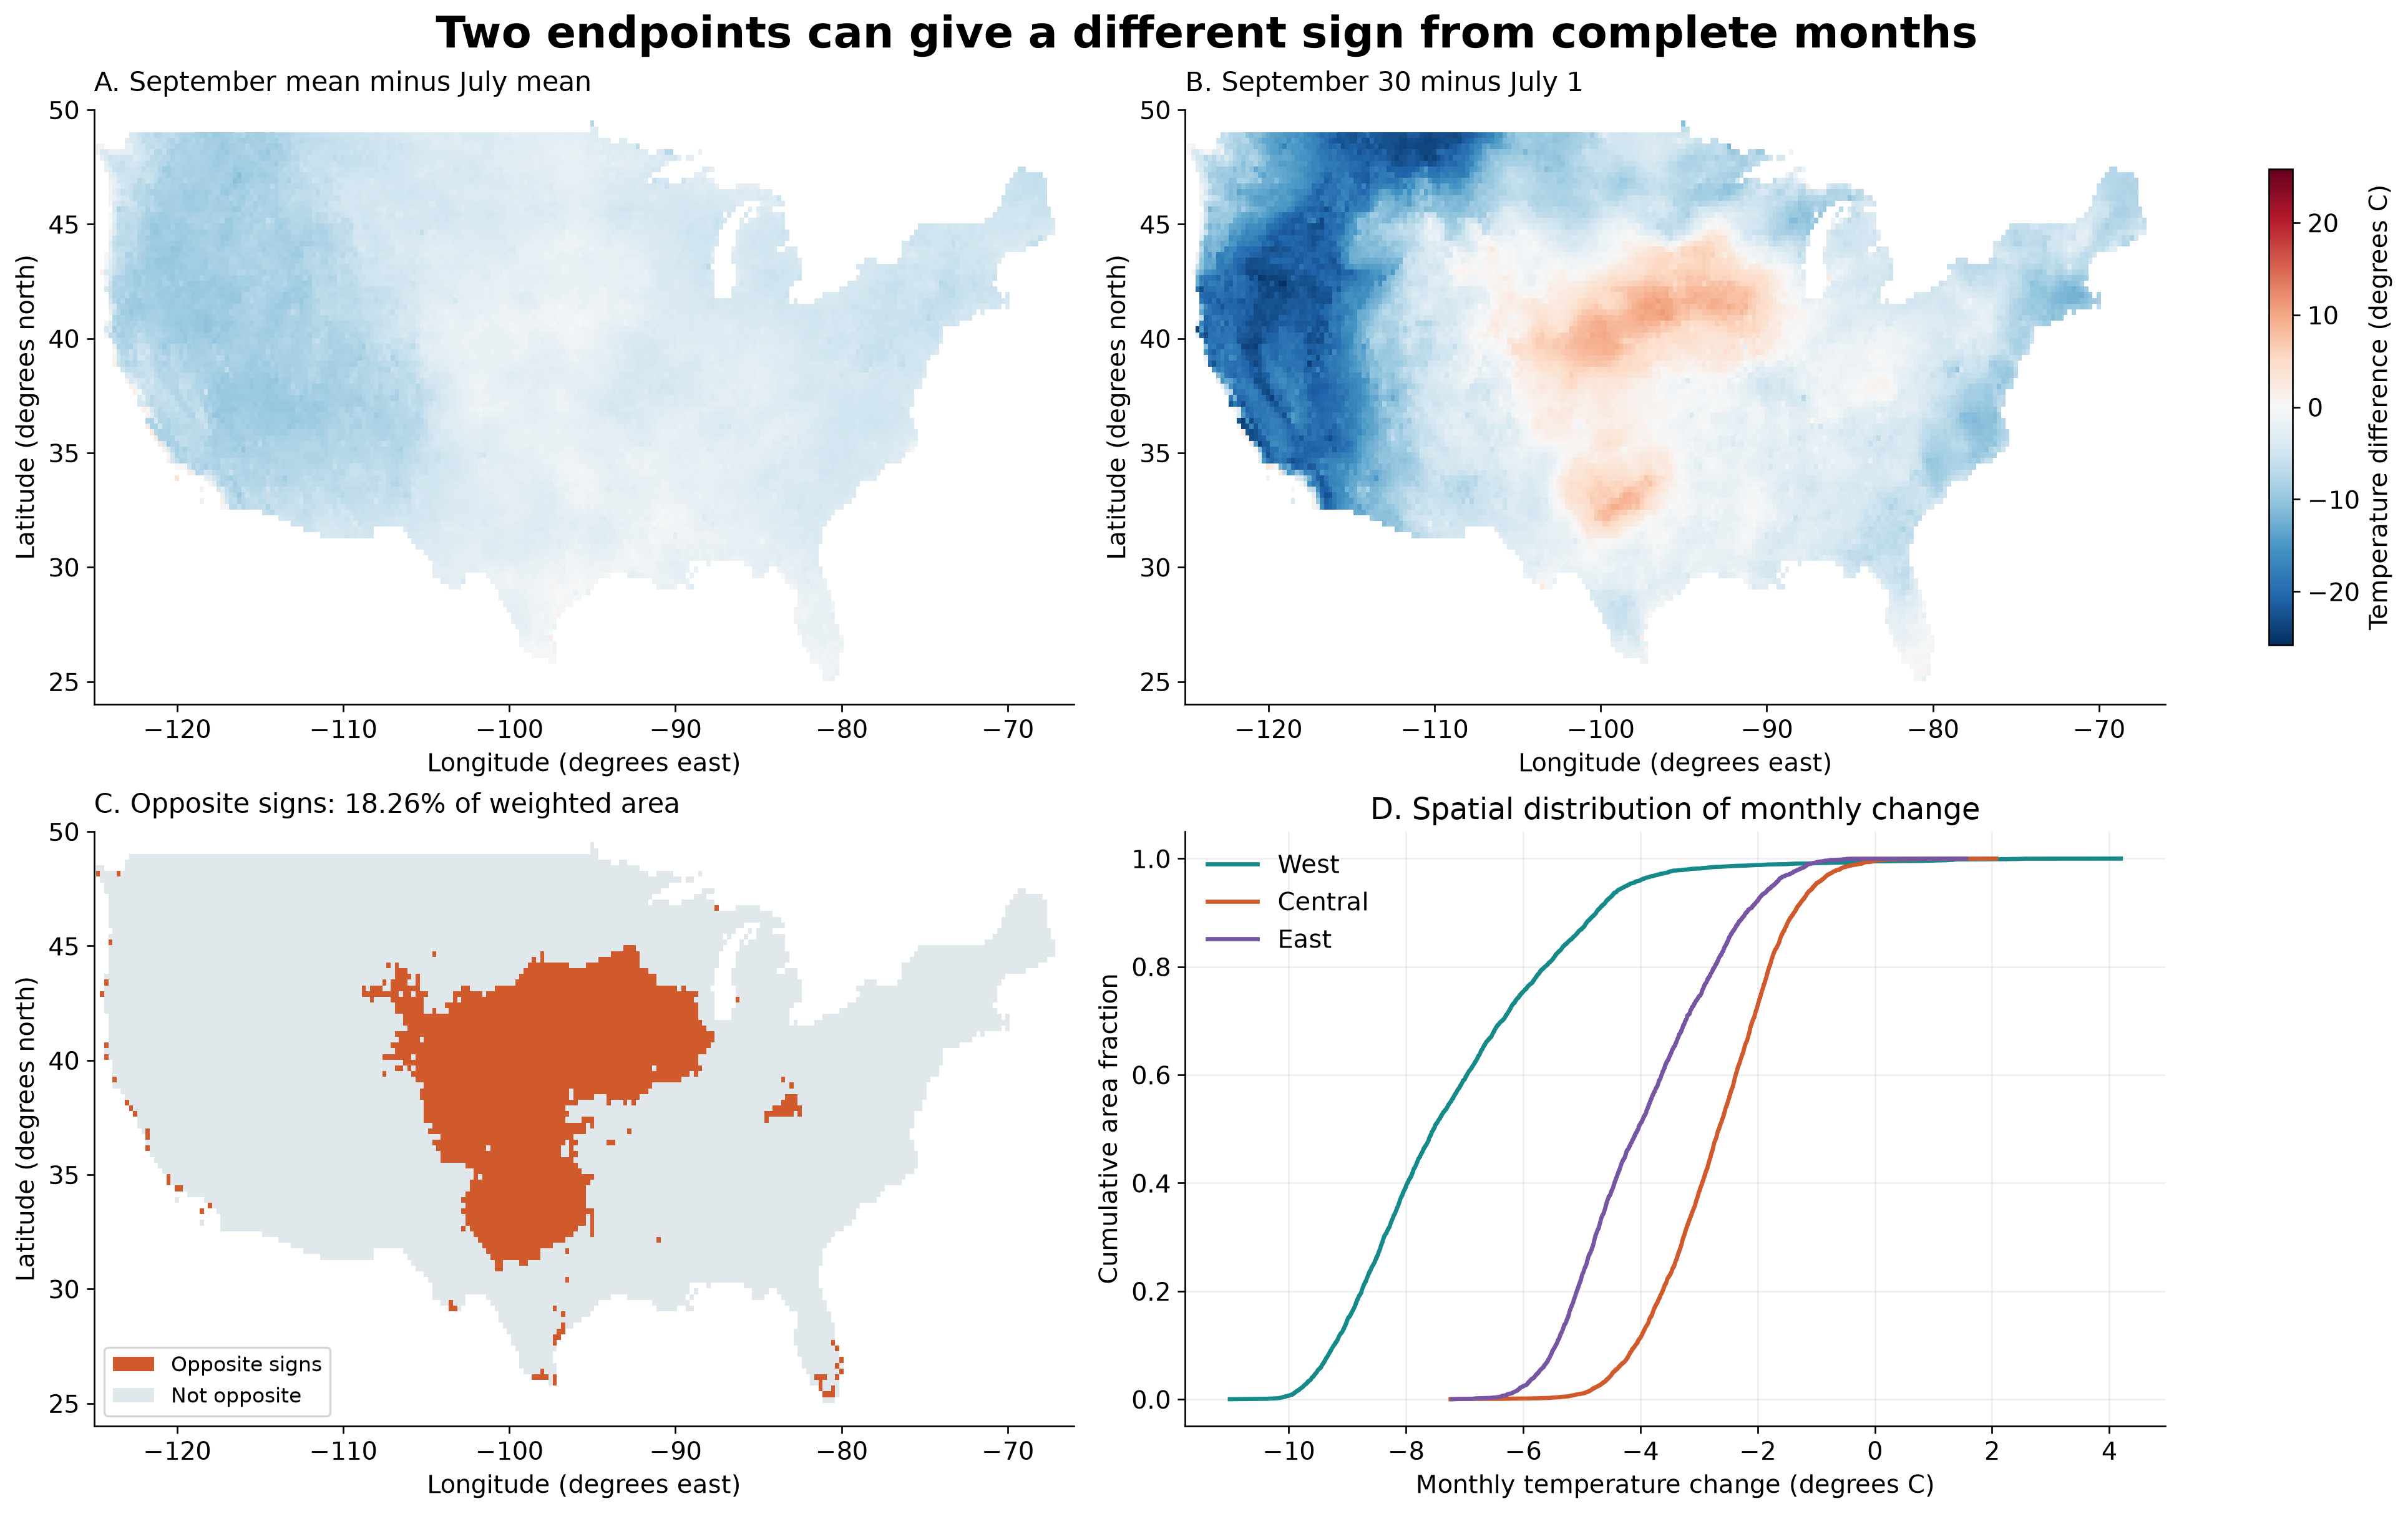
\includegraphics[width=\textwidth,height=0.55\textheight,keepaspectratio]{Fig22.png}

\caption{Endpoint and complete-month differences have opposite signs over 18.26\% of area. {\footnotesize \href{https://aithal007.github.io/DV_assignment2/figures.html\#fig22}{\textcolor{accent}{\underline{View figure and interpretation online}}}}}\label{fig:22}

\end{figure*}

\noindent\textit{How to read the graph.} A/B compare monthly and endpoint differences with shared limits. C marks opposite signs; D shows area-weighted monthly-change distributions.

\paragraph{Question.} Can two daily snapshots describe a whole month's change?



\paragraph{Visual encoding.} A: complete-month difference; B: September 30 minus July 1, with the same zero-centered limits. C: orange marks opposite signs. D: area-weighted cumulative distributions of monthly changes by longitude sector.



\paragraph{Why this visualization.} Three maps show overall cooling but make small spatial differences difficult to compare. A diverging colormap suits a difference map because zero is a meaningful reference: it separates cooling from warming. Symmetric color limits show the sign and size of change around that neutral center. The cumulative curves show how widespread each change is within longitude bands, rather than reducing each band to one mean.



\paragraph{Interpretation.} A/B use the same symmetric color limits for complete-month and endpoint changes. Monthly September-minus-July means cool over 99.66\% of weighted area, with mean change -4.64 C. C directly marks the 18.26\% where September 30 minus July 1 has the opposite sign. D shows how monthly cooling varies across longitude sectors.

Thus the endpoint discrepancy is visible rather than only stated. Two selected weather states can misrepresent the direction of complete-month change at a location. Comparing matched footprints and a zero-centered diverging scale separates this sampling effect from a color-scale change; the cumulative curves prevent one area mean from concealing spatial variation.



\paragraph{Scope and reading note.} The result describes this 2023 interval and sampled area; it is not a long-term climate trend.



\takeaway{Two endpoint days can misrepresent change across the full interval. Their change sign disagrees with the complete-month comparison over 18.26\% of the study area. Use all days when the claim concerns monthly conditions rather than two weather states.

}

\noindent\textit{Analytical recommendation.} Check whether endpoint dates reverse the complete-month direction.

\subsection{Fig. 23: Monthly rain totals and five-day bursts}

\begin{figure*}[!tb]\centering

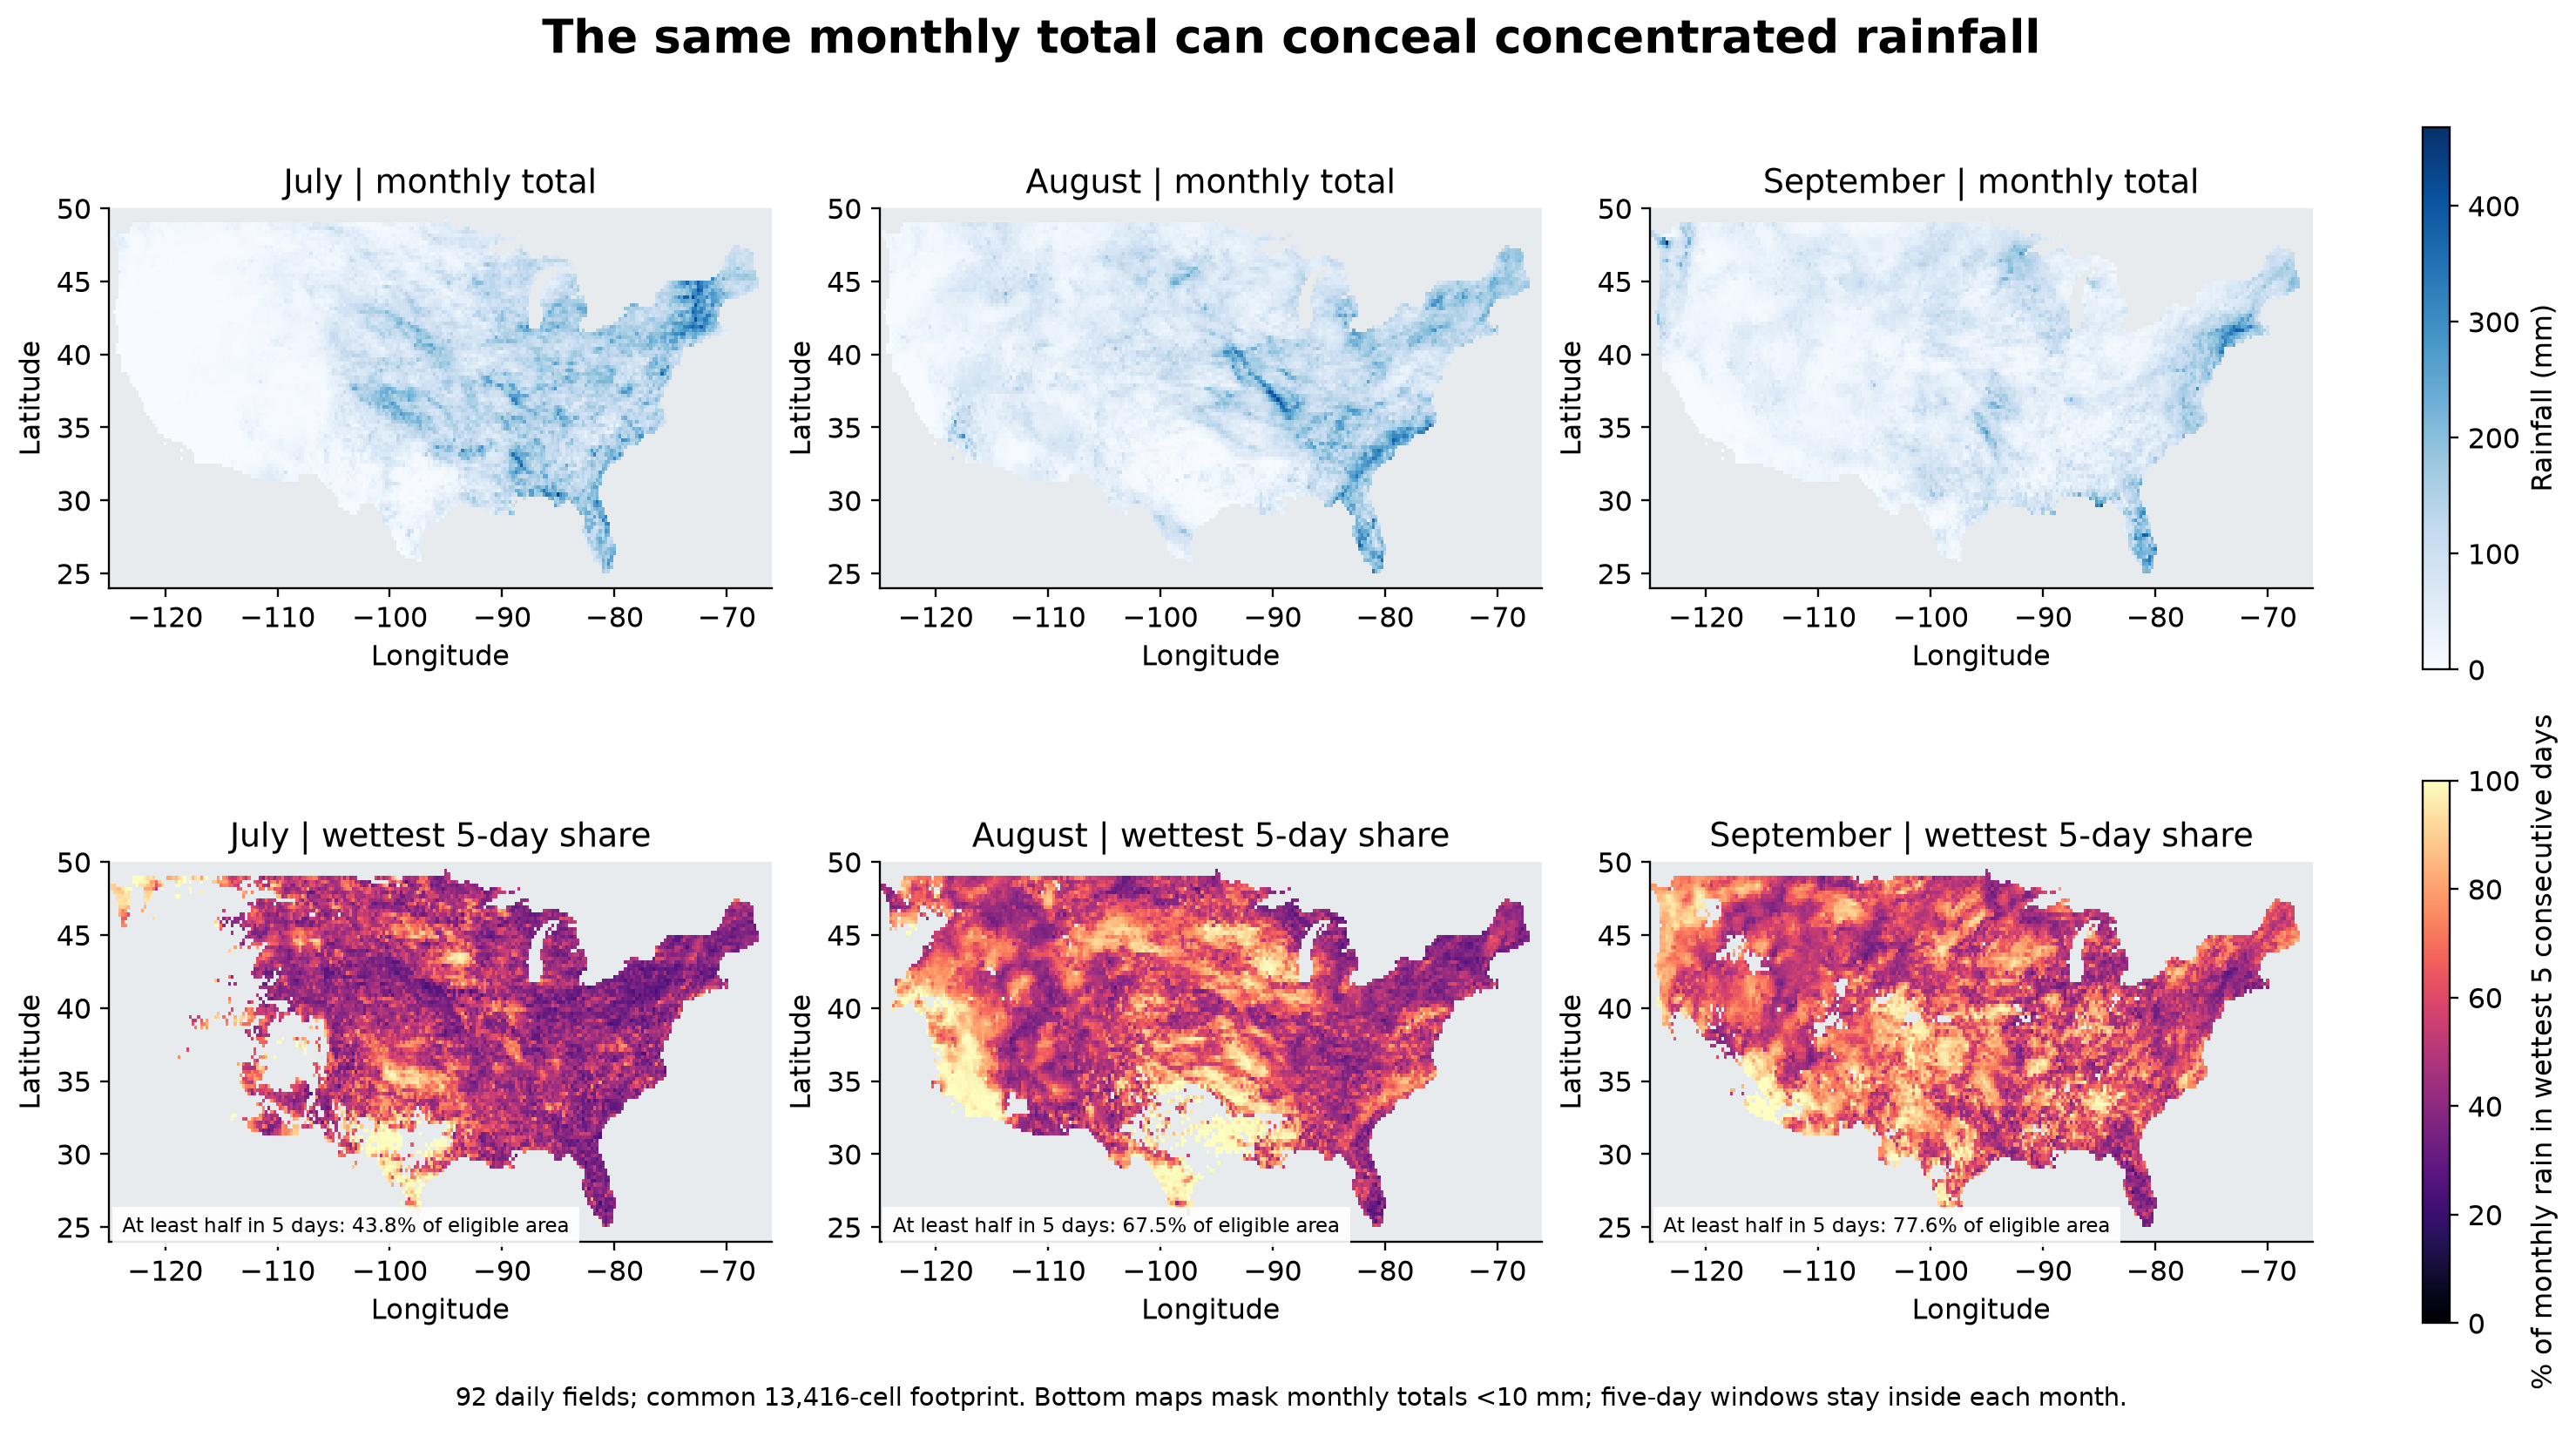
\includegraphics[width=0.88\textwidth,height=0.44\textheight,keepaspectratio]{Fig23.png}

\caption{Similar monthly rain totals conceal different five-day concentration. {\footnotesize \href{https://aithal007.github.io/DV_assignment2/figures.html\#fig23}{\textcolor{accent}{\underline{View figure and interpretation online}}}}}\label{fig:23}

\end{figure*}

\noindent\textit{How to read the graph.} Top: monthly rain totals. Bottom: wettest five-day share, restricted to cells with at least 10 mm monthly rain. Masks change eligible footprints.

\paragraph{Question.} Can similar monthly totals come from different rainfall timing?



\paragraph{Visual encoding.} The top row shows monthly rain totals on one scale. The bottom row shows the share of each month's rain that falls in its wettest five consecutive days. Cells with less than 10 mm monthly rain are masked in the bottom row.



\paragraph{Why this visualization.} A monthly rainfall total cannot distinguish steady rain from a short burst. The second row adds the share falling in the wettest five consecutive days. Keeping total and concentration separate avoids calling a very small rain amount a major event simply because all of it fell at once.



\paragraph{Interpretation.} July and August have similar weighted rain totals, 75.26 and 75.82 mm, but different timing. Among cells with monthly total at least 10 mm, 43.8\% of eligible July area gets at least half its rain in one five-day window, versus 67.5\% in August and 77.6\% in September. September's total is lower, 57.08 mm.

The minimum-total mask avoids ratios dominated by tiny denominators; eligible footprints differ (74.75\%, 92.32\%, 94.09\%). Concentration also depends on wet-day count: a cell with few rain days can have a large five-day share without a sustained episode. Read the ratio with totals and daily timing, rather than interpreting it directly as event duration or hazard.



\paragraph{Scope and reading note.} Windows stay inside each month. The eligible area differs by month, and this measure does not establish flooding.



\takeaway{Monthly rainfall amount cannot identify how rain arrived. Similar July-August totals conceal different five-day concentration, and September has the largest concentration share despite a lower total. Compare amount with timing, using the explicitly eligible area for each month.

}

\noindent\textit{Analytical recommendation.} Separate monthly amount, wet-day count and concentration of timing.

\subsection{Fig. 24: Where hot days are frequent}

\begin{figure*}[!tb]\centering

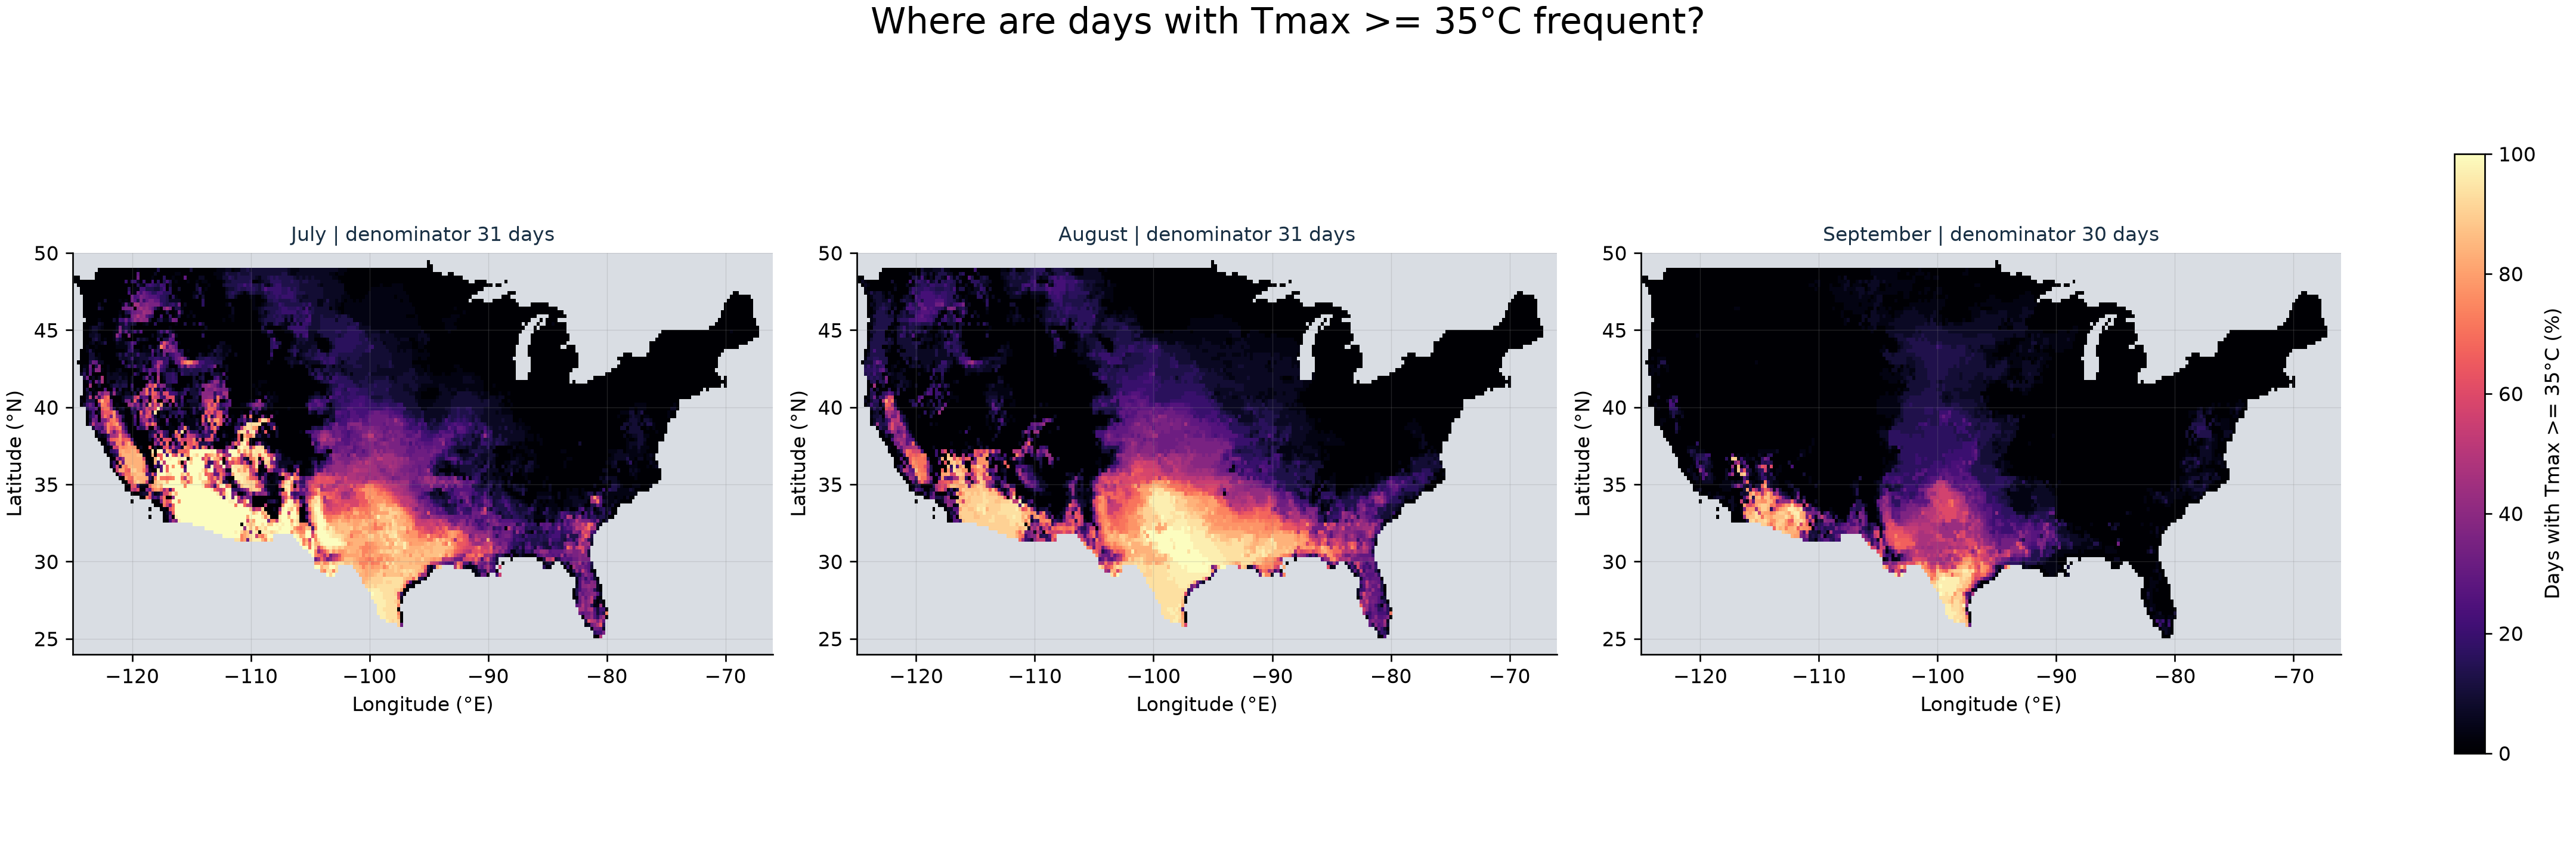
\includegraphics[width=\textwidth,height=0.49\textheight,keepaspectratio]{Fig24.png}

\caption{Repeated hot days remain spatially concentrated despite seasonal cooling. {\footnotesize \href{https://aithal007.github.io/DV_assignment2/figures.html\#fig24}{\textcolor{accent}{\underline{View figure and interpretation online}}}}}\label{fig:24}

\end{figure*}

\noindent\textit{How to read the graph.} Each month maps the percentage of its days at or above 35 C. Shared colors compare repetition; zero is a measured frequency.

\paragraph{Question.} Where do daily maximum temperatures often reach 35\textdegree{}C?



\paragraph{Visual encoding.} Each map shows the percentage of days in a month with daily maximum temperature at least 35\textdegree{}C. The three maps share one 0-100\% scale.



\paragraph{Why this visualization.} A monthly mean temperature does not count how often a chosen hot threshold was exceeded. Frequency maps use all days and preserve location, making repeated heat distinguishable from one selected hot day. The fixed percentage scale lets July, August and September be compared directly.



\paragraph{Interpretation.} The weighted mean frequency of Tmax >=35 C falls from 22.8\% of July days to 8.9\% of September days. The spatial colors show where repeated threshold exceedance remains concentrated, providing evidence that is absent from the monthly mean temperature alone.

The denominator is each month's number of days, so 31 versus 30 days does not mechanically create the contrast. A 50\% cell crosses the chosen threshold on half its days, but its warm days may be consecutive or scattered. Thus these maps establish repetition and location, while the persistence map/calendar establish sequence and duration. The 35 C threshold is a declared descriptive definition rather than a universal heat-risk criterion; the final sensitivity panel checks how that choice affects the counts.



\paragraph{Scope and reading note.} The 35\textdegree{}C threshold is a chosen study definition. Frequency alone does not show whether hot days form one continuous run.



\takeaway{Hot-day frequency reveals repeated heat that a monthly mean or one selected date cannot count. Its decline from July to September measures occurrence, while the maps retain location. Frequency still leaves the ordering of those days unresolved.

}

\noindent\textit{Analytical recommendation.} Use persistence views to distinguish scattered hot days from continuous spells.

\subsection{Fig. 25: Hovmoller diagrams: daily departures and rain across longitude}

\begin{figure*}[!tb]\centering

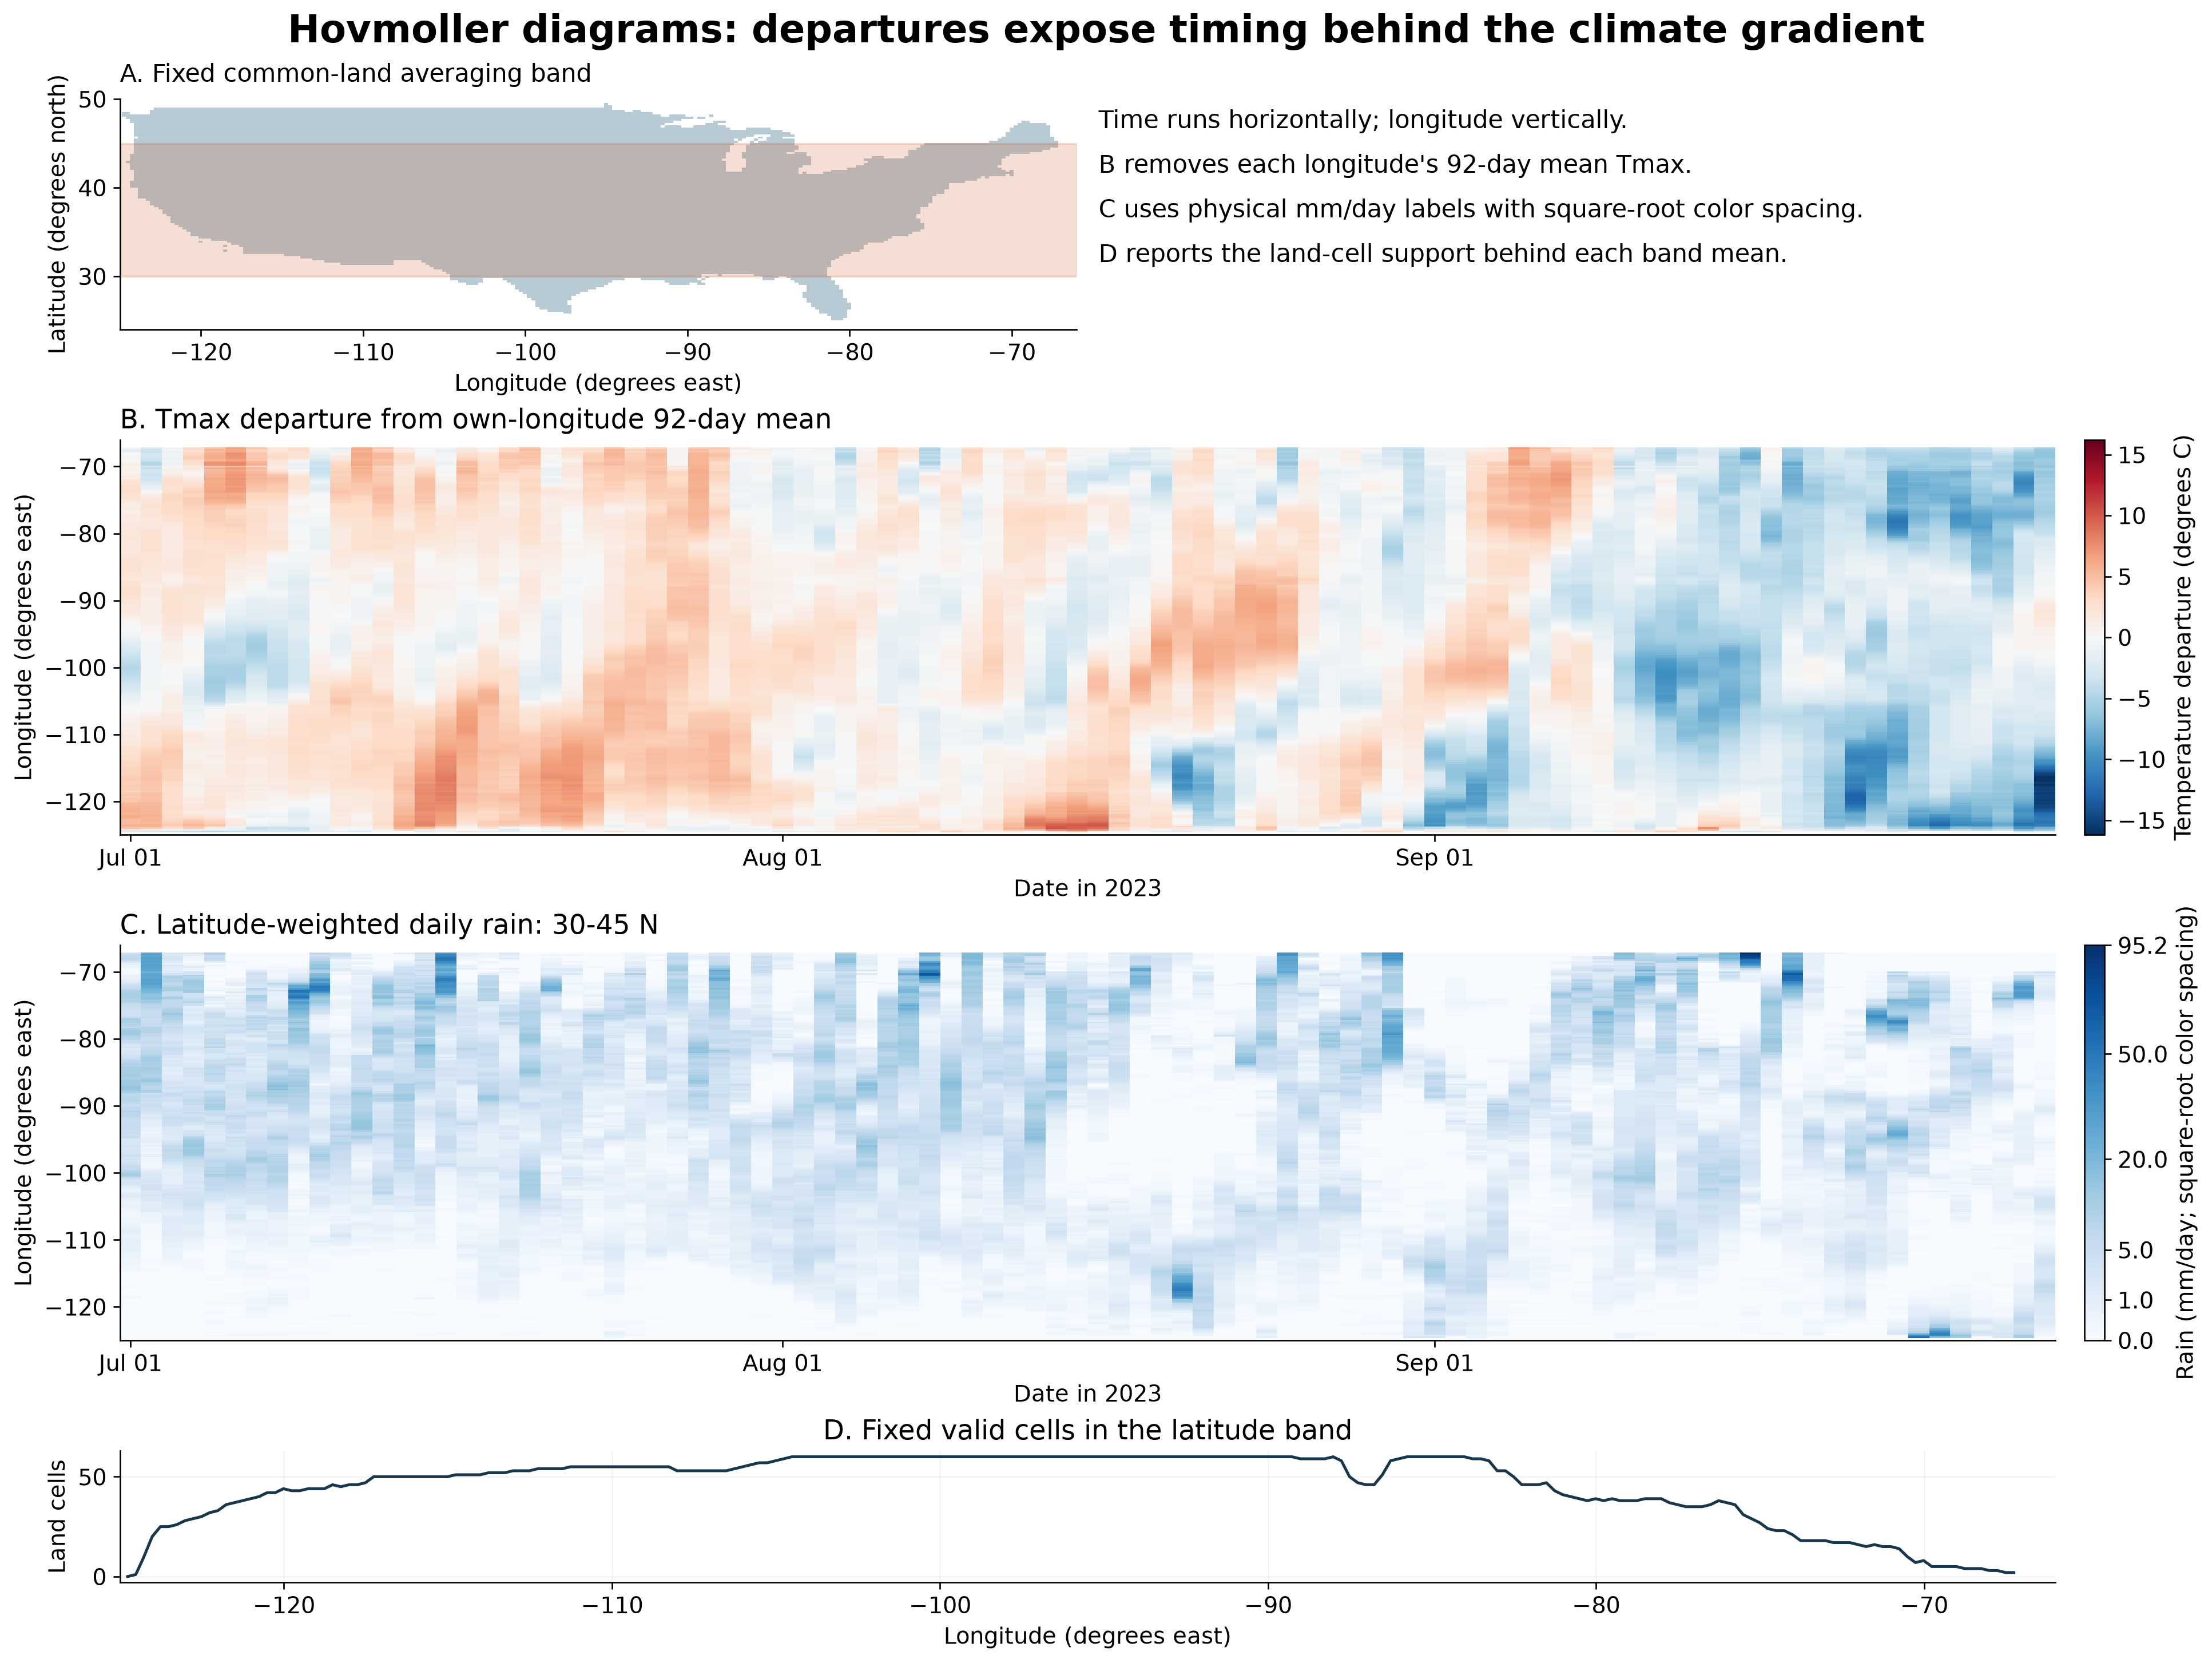
\includegraphics[width=\textwidth,height=0.65\textheight,keepaspectratio]{Fig25.png}

\caption{Longitude-centered departures reveal timing; coastal rain extremes can have sparse spatial support. {\footnotesize \href{https://aithal007.github.io/DV_assignment2/figures.html\#fig25}{\textcolor{accent}{\underline{View figure and interpretation online}}}}}\label{fig:25}

\end{figure*}

\noindent\textit{How to read the graph.} A locates 30-45 N. B/C place date horizontally and longitude vertically; colors show period-mean Tmax departures and rain. D reports land-cell support.

\paragraph{Question.} When and where do warm and rainy periods occur?



\paragraph{Visual encoding.} A identifies the fixed 30-45 N band. In B/C, horizontal position is date and vertical position longitude. B shows departure from each longitude's own period mean; C shows actual rain with square-root color spacing. D gives the contributing-cell count.



\paragraph{Why this visualization.} Maps preserve location but require many frames to show all 92 days. A time-longitude diagram keeps every date visible in one view. Averaging across latitude makes room for that time axis, so episodes can be compared by their dates and east-west extent rather than remembered across an animation.



\paragraph{Interpretation.} This Hovmoller display retains daily time-longitude structure \cite{ref11}. Time is horizontal and longitude vertical across the fixed 30-45 N band. Panel B subtracts each longitude's 92-day mean Tmax, removing the fixed east-west gradient to expose warm/cool departures. Persistent positive anomalies across 110-120 W in July reflect the historic Southwest heat dome documented by NOAA \cite{ref9}.

In Panel C, the largest latitude-weighted rain mean is 95.20 mm/day on September 16 at 67.27 W (averaging two valid coastal cells, 94.10 and 96.30 mm/day; color spacing is square-root transformed). Panel D reports longitude support (1-60 cells). Synoptic context connects the August 22 Texas rainfall to the landfall of Tropical Storm Harold \cite{ref16}, and the September 16 Maine coastal maximum to Hurricane Lee \cite{ref17}. Harold's heaviest coastal rain fell south of the 30-45 N band (about 26-29 N), so these band averages track its northern extent rather than its coastal core; the September 16 Maine maximum lies inside the band. Latitude-band averages illustrate event timing and longitude extent while aggregating local storm structures.



\paragraph{Scope and reading note.} Averaging across latitude hides north-south differences. Reading across columns does not by itself track a moving storm.



\takeaway{Retaining every date exposes episodes smoothed away by monthly maps. The time-longitude view locates their timing and east-west extent, but latitude averaging removes north-south detail. Return to maps before interpreting a band as a specific event location or track.

}

\noindent\textit{Analytical recommendation.} Check baseline and spatial support before interpreting time-longitude streaks.

\section{Wind direction and magnitude}

Quiver maps locate the flow; monthly direction distributions describe how often different winds occur.



\subsection{Fig. 26: Quiver: readable sampling and arrow-length comparisons}

\begin{figure*}[!tb]\centering

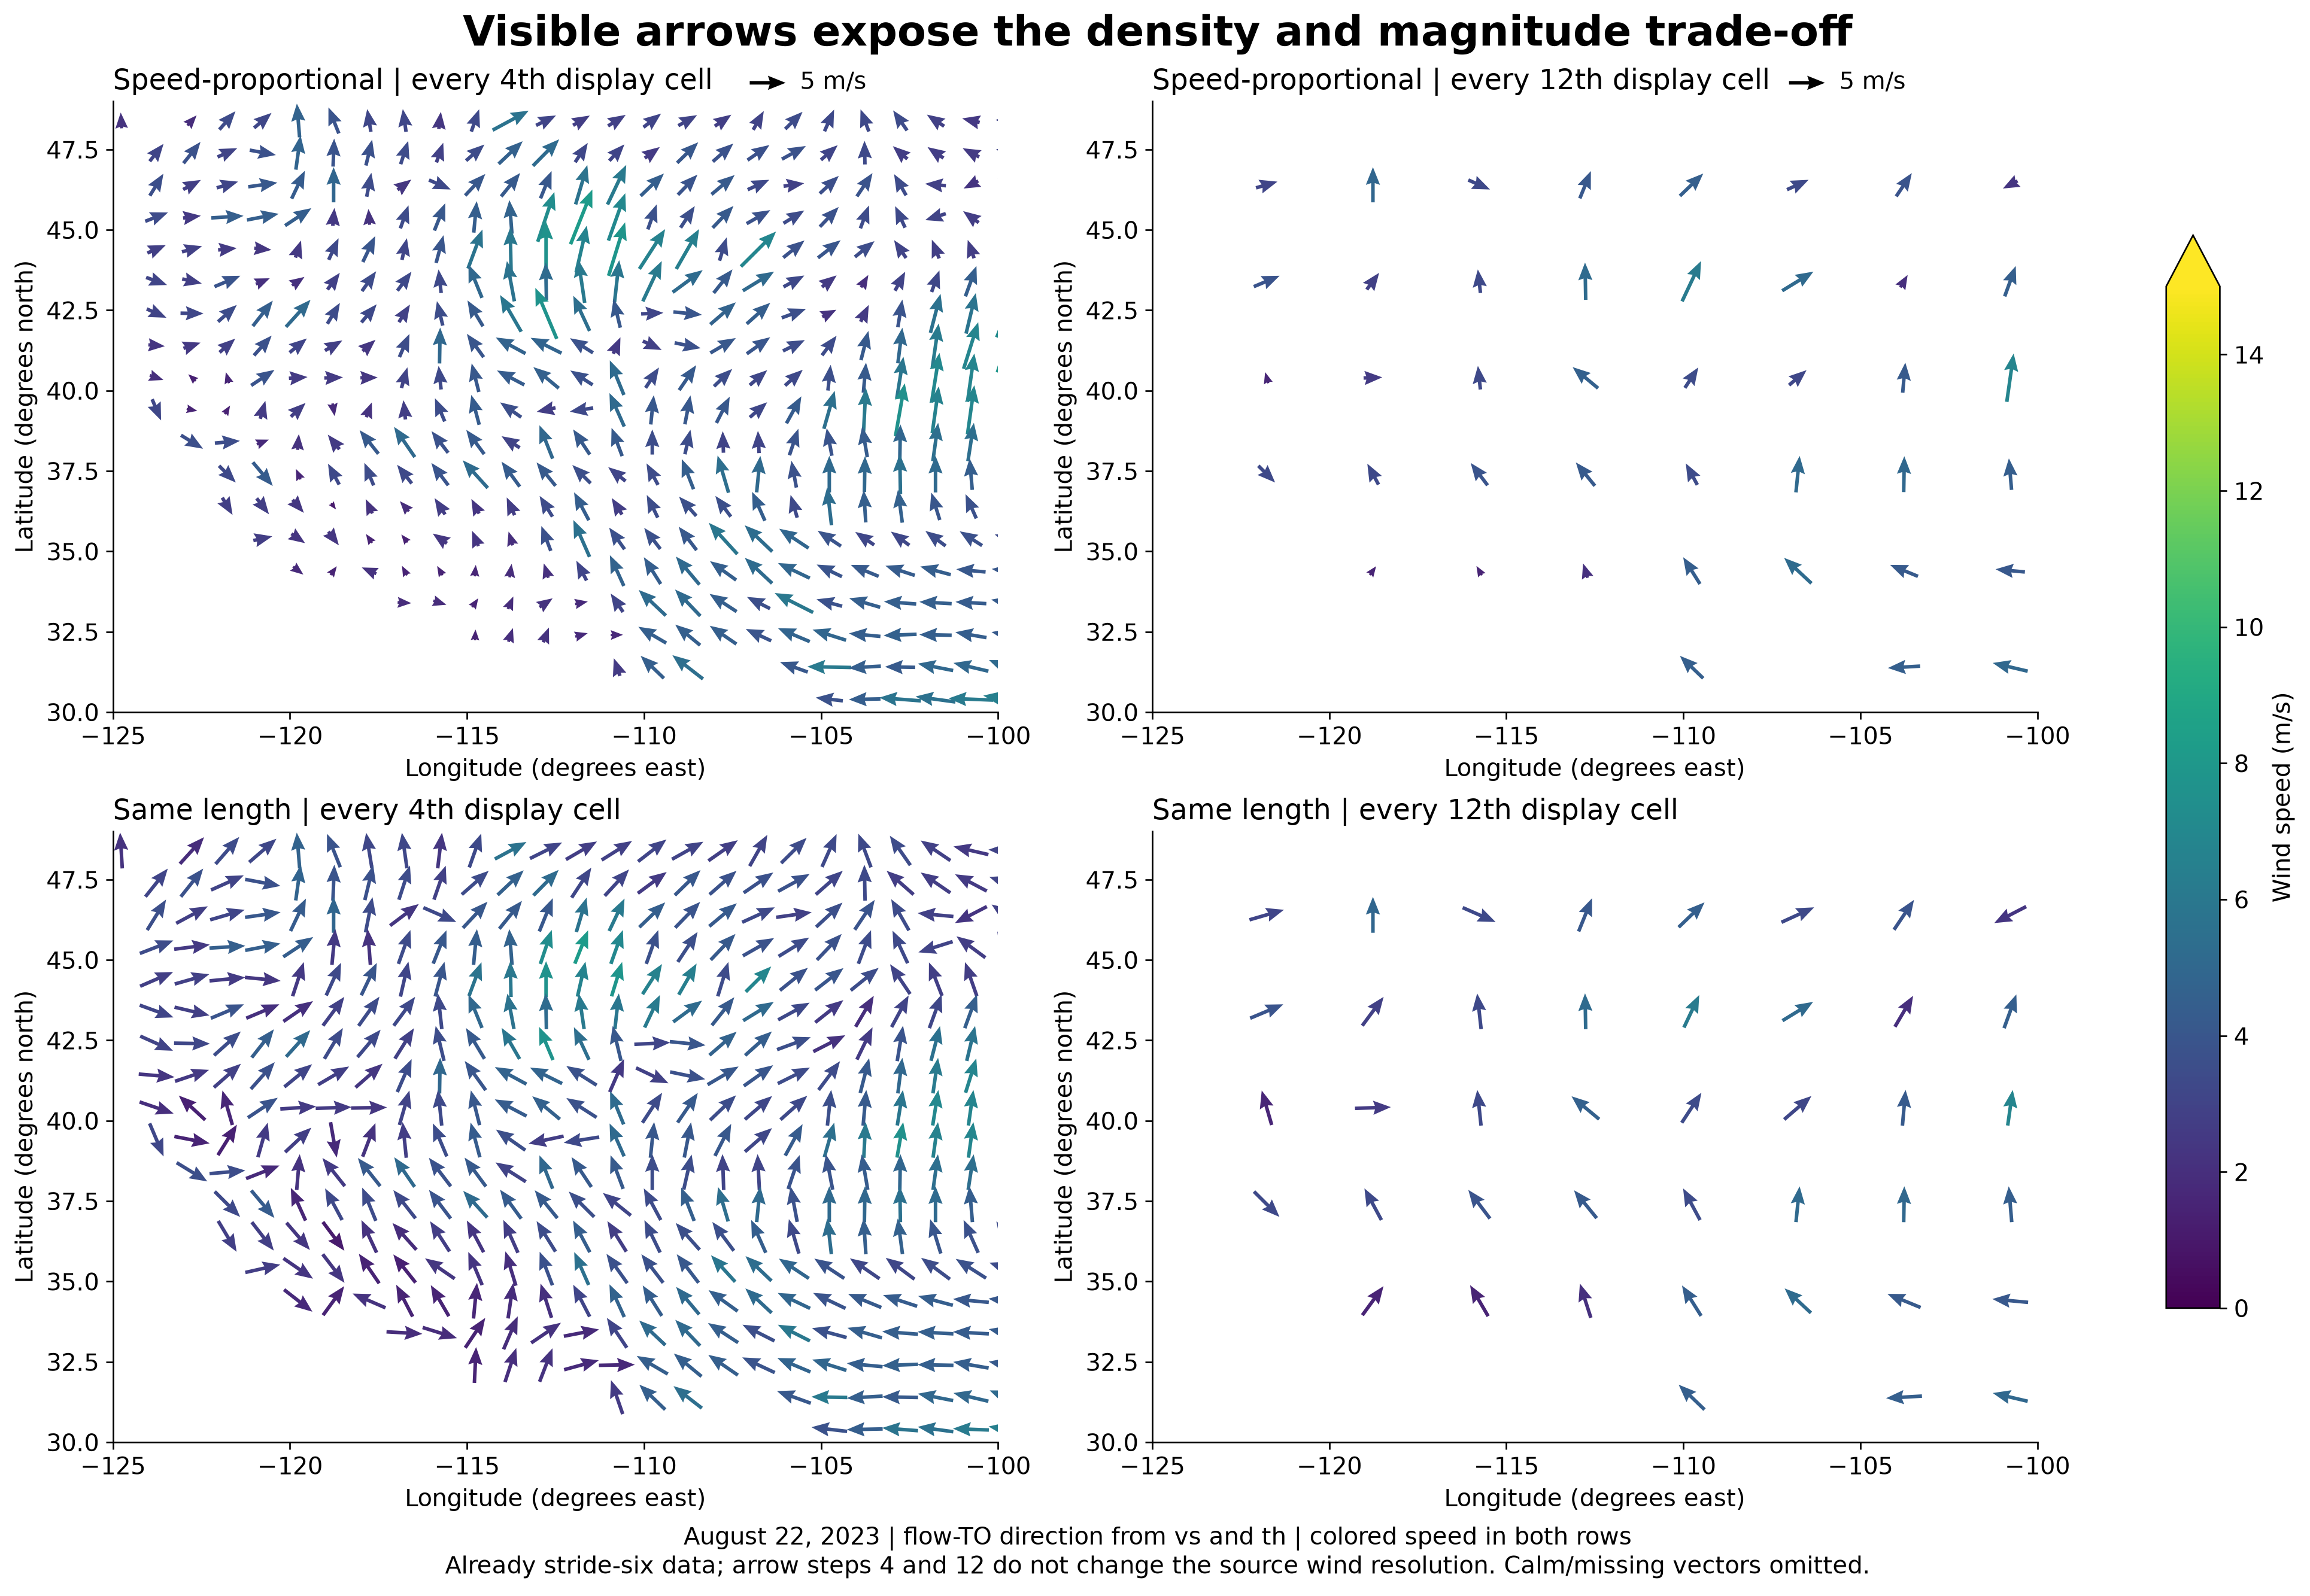
\includegraphics[width=\textwidth,height=0.47\textheight,keepaspectratio]{Fig26.png}

\caption{Thinning removes locations; equal arrow lengths remove magnitude encoding. {\footnotesize \href{https://aithal007.github.io/DV_assignment2/figures.html\#fig26}{\textcolor{accent}{\underline{View figure and interpretation online}}}}}\label{fig:26}

\end{figure*}

\noindent\textit{How to read the graph.} Columns sample every fourth/twelfth display cell. Upper arrow lengths encode speed; lower lengths are equal. Colors encode speed throughout; keys identify 5 m/s.

\paragraph{Question.} How do sampling and arrow length affect readability?



\paragraph{Visual encoding.} Columns sample every fourth/twelfth point of the already stride-six cache. Upper arrows have speed-proportional lengths; lower arrows have equal lengths. Color shows speed in both rows; keys identify the upper physical scale.



\paragraph{Why this visualization.} An arrow map can become unreadable before it becomes informative. Holding the wind field fixed while varying spacing shows how much local detail is traded for legibility. Comparing speed-scaled and equal-length arrows also separates the tasks of reading direction and reading magnitude.



\paragraph{Interpretation.} Two sampling densities compare every fourth and twelfth display cell on the August 22 western-US field. Speed-proportional arrows retain a 5 m/s physical key; equal-length arrows prioritize directional flow while color encodes speed throughout. Sparse sampling clarifies general circulation without introducing interpolation artifacts.

The required variables are \path{vs} (10 m speed) and \path{th} (10 m FROM-direction). After angle conversion to radians, $u = -v_s \sin(\theta)$, $v = -v_s \cos(\theta)$ gives flow-TO components. Display bearings account for longitude scale and map aspect. The comparison isolates symbol density and length encoding; it cannot reveal finer wind resolution or trajectories absent from the data \cite{ref1}.



\paragraph{Scope and reading note.} These are daily wind values at 10 m, not gusts or paths followed by air parcels.



\takeaway{Arrow spacing and length determine which wind questions are readable. Sparse sampling clarifies directions while omitting locations; equal lengths emphasize direction and speed-scaled lengths add magnitude. Interpret the vector convention and speed colors with the chosen design.

}

\noindent\textit{Analytical recommendation.} Choose arrow density and length encoding together to preserve readable direction.

\subsection{Fig. 27: Monthly wind-direction distributions}

\begin{figure*}[!tb]\centering

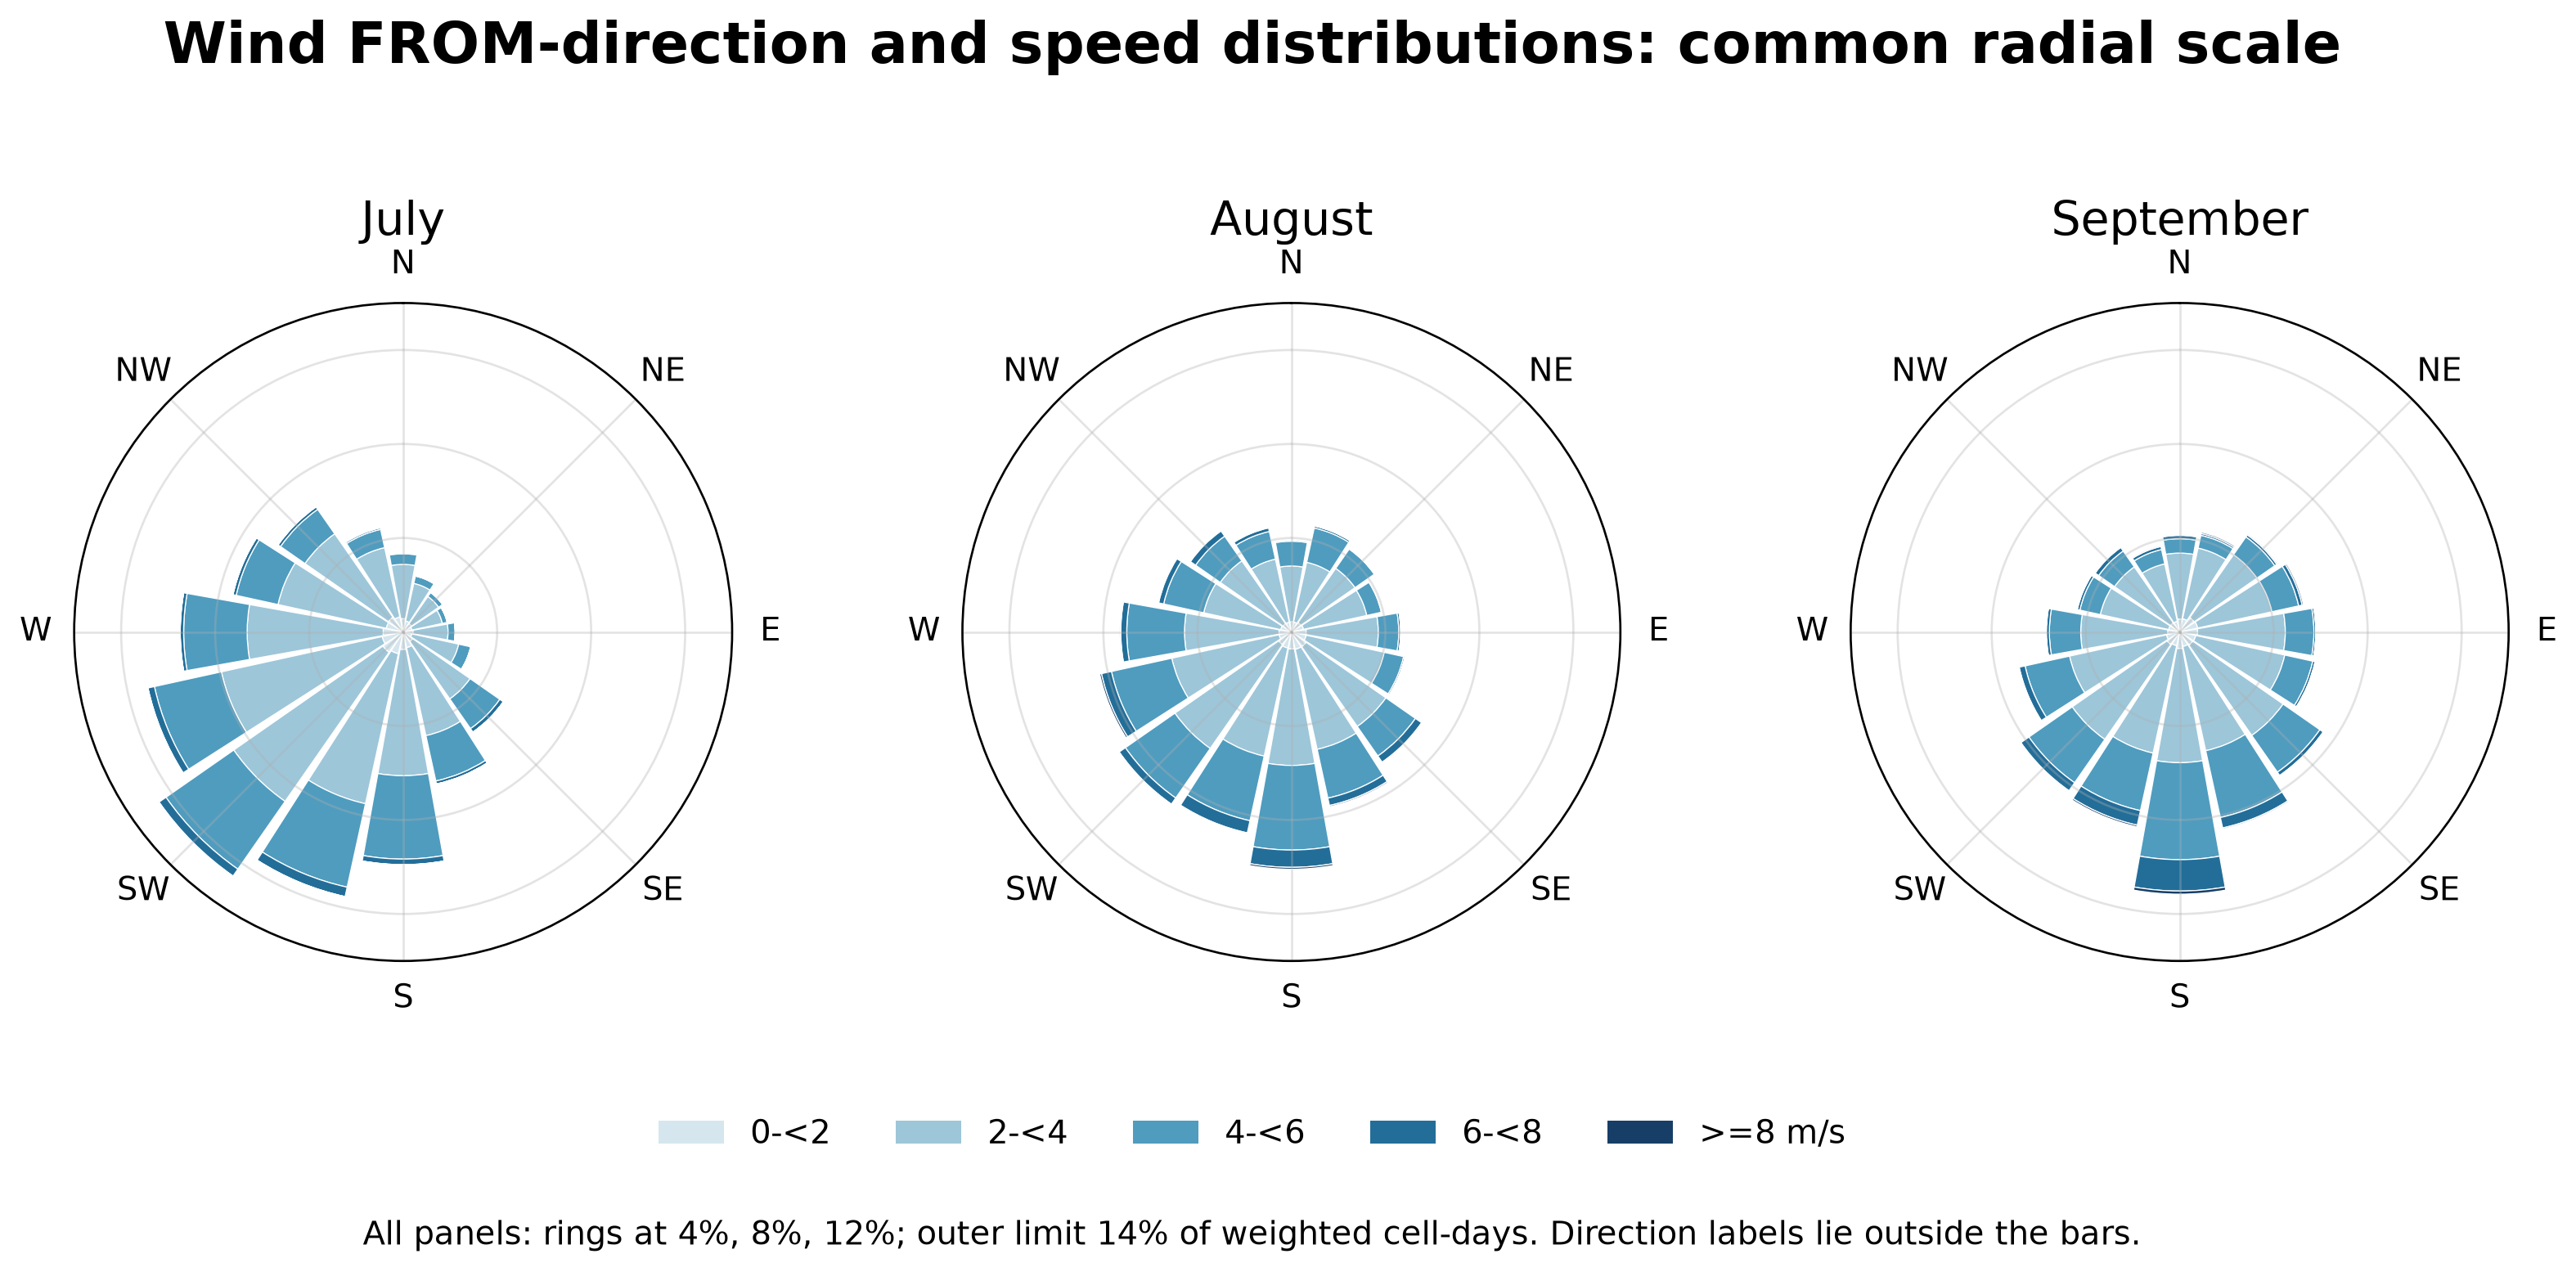
\includegraphics[width=\textwidth,height=0.42\textheight,keepaspectratio]{Fig27.png}

\caption{Common-scale roses expose a monthly shift in source direction. {\footnotesize \href{https://aithal007.github.io/DV_assignment2/figures.html\#fig27}{\textcolor{accent}{\underline{View figure and interpretation online}}}}}\label{fig:27}

\end{figure*}

\noindent\textit{How to read the graph.} Each rose bins FROM-direction; stacked colors bin speed. Ring frequencies and the 14\% radial maximum are common across all three months.

\paragraph{Question.} Does one pooled wind summary hide monthly differences?



\paragraph{Visual encoding.} Each rose groups a month's grid-cell days by wind source direction. Stacked colors show speed ranges. The same radial scale gives the percentage of each month's weighted grid-cell days.



\paragraph{Why this visualization.} Quiver maps show where wind points, but not how often each source direction occurs across a month. Wind roses collect those directions into sectors and divide each sector by speed. Separate monthly panels and a common radial scale reveal changes that one pooled seasonal rose would hide.



\paragraph{Interpretation.} July's dominant source-direction sector is southwest, shifting southward in August and September. All roses use an identical 14\% outer frequency limit, with ring values positioned outside bars to prevent visual clutter. Stacked colors show speed class contributions to each directional bin.

Each percentage uses weighted grid-cell days in that month, not just days at one station. Equal radial scales make the seasonal shift comparable, while the common legend prevents color reinterpretation. This pooled direction distribution complements the quiver maps: it reveals frequency changes but deliberately gives up exact location.



\paragraph{Scope and reading note.} Read radial height as frequency. Near-calm directions carry little physical meaning.



\takeaway{Wind direction and strength distributions change within the three-month interval. Monthly roses expose a source-direction shift that a pooled seasonal summary could hide. Their common radial scale supports frequency comparison, while maps remain necessary to locate the winds.

}

\noindent\textit{Analytical recommendation.} Compare pooled direction frequencies, then return to maps for location.

\section{Coincidence, frequency and persistence}

Aligned fields identify joint conditions, full-period counts establish occurrence, and the daily calendar explains why equal frequencies can have unequal run lengths.



\subsection{Fig. 28: Temperature, rain and wind on the same dates}

\begin{figure*}[!tb]\centering

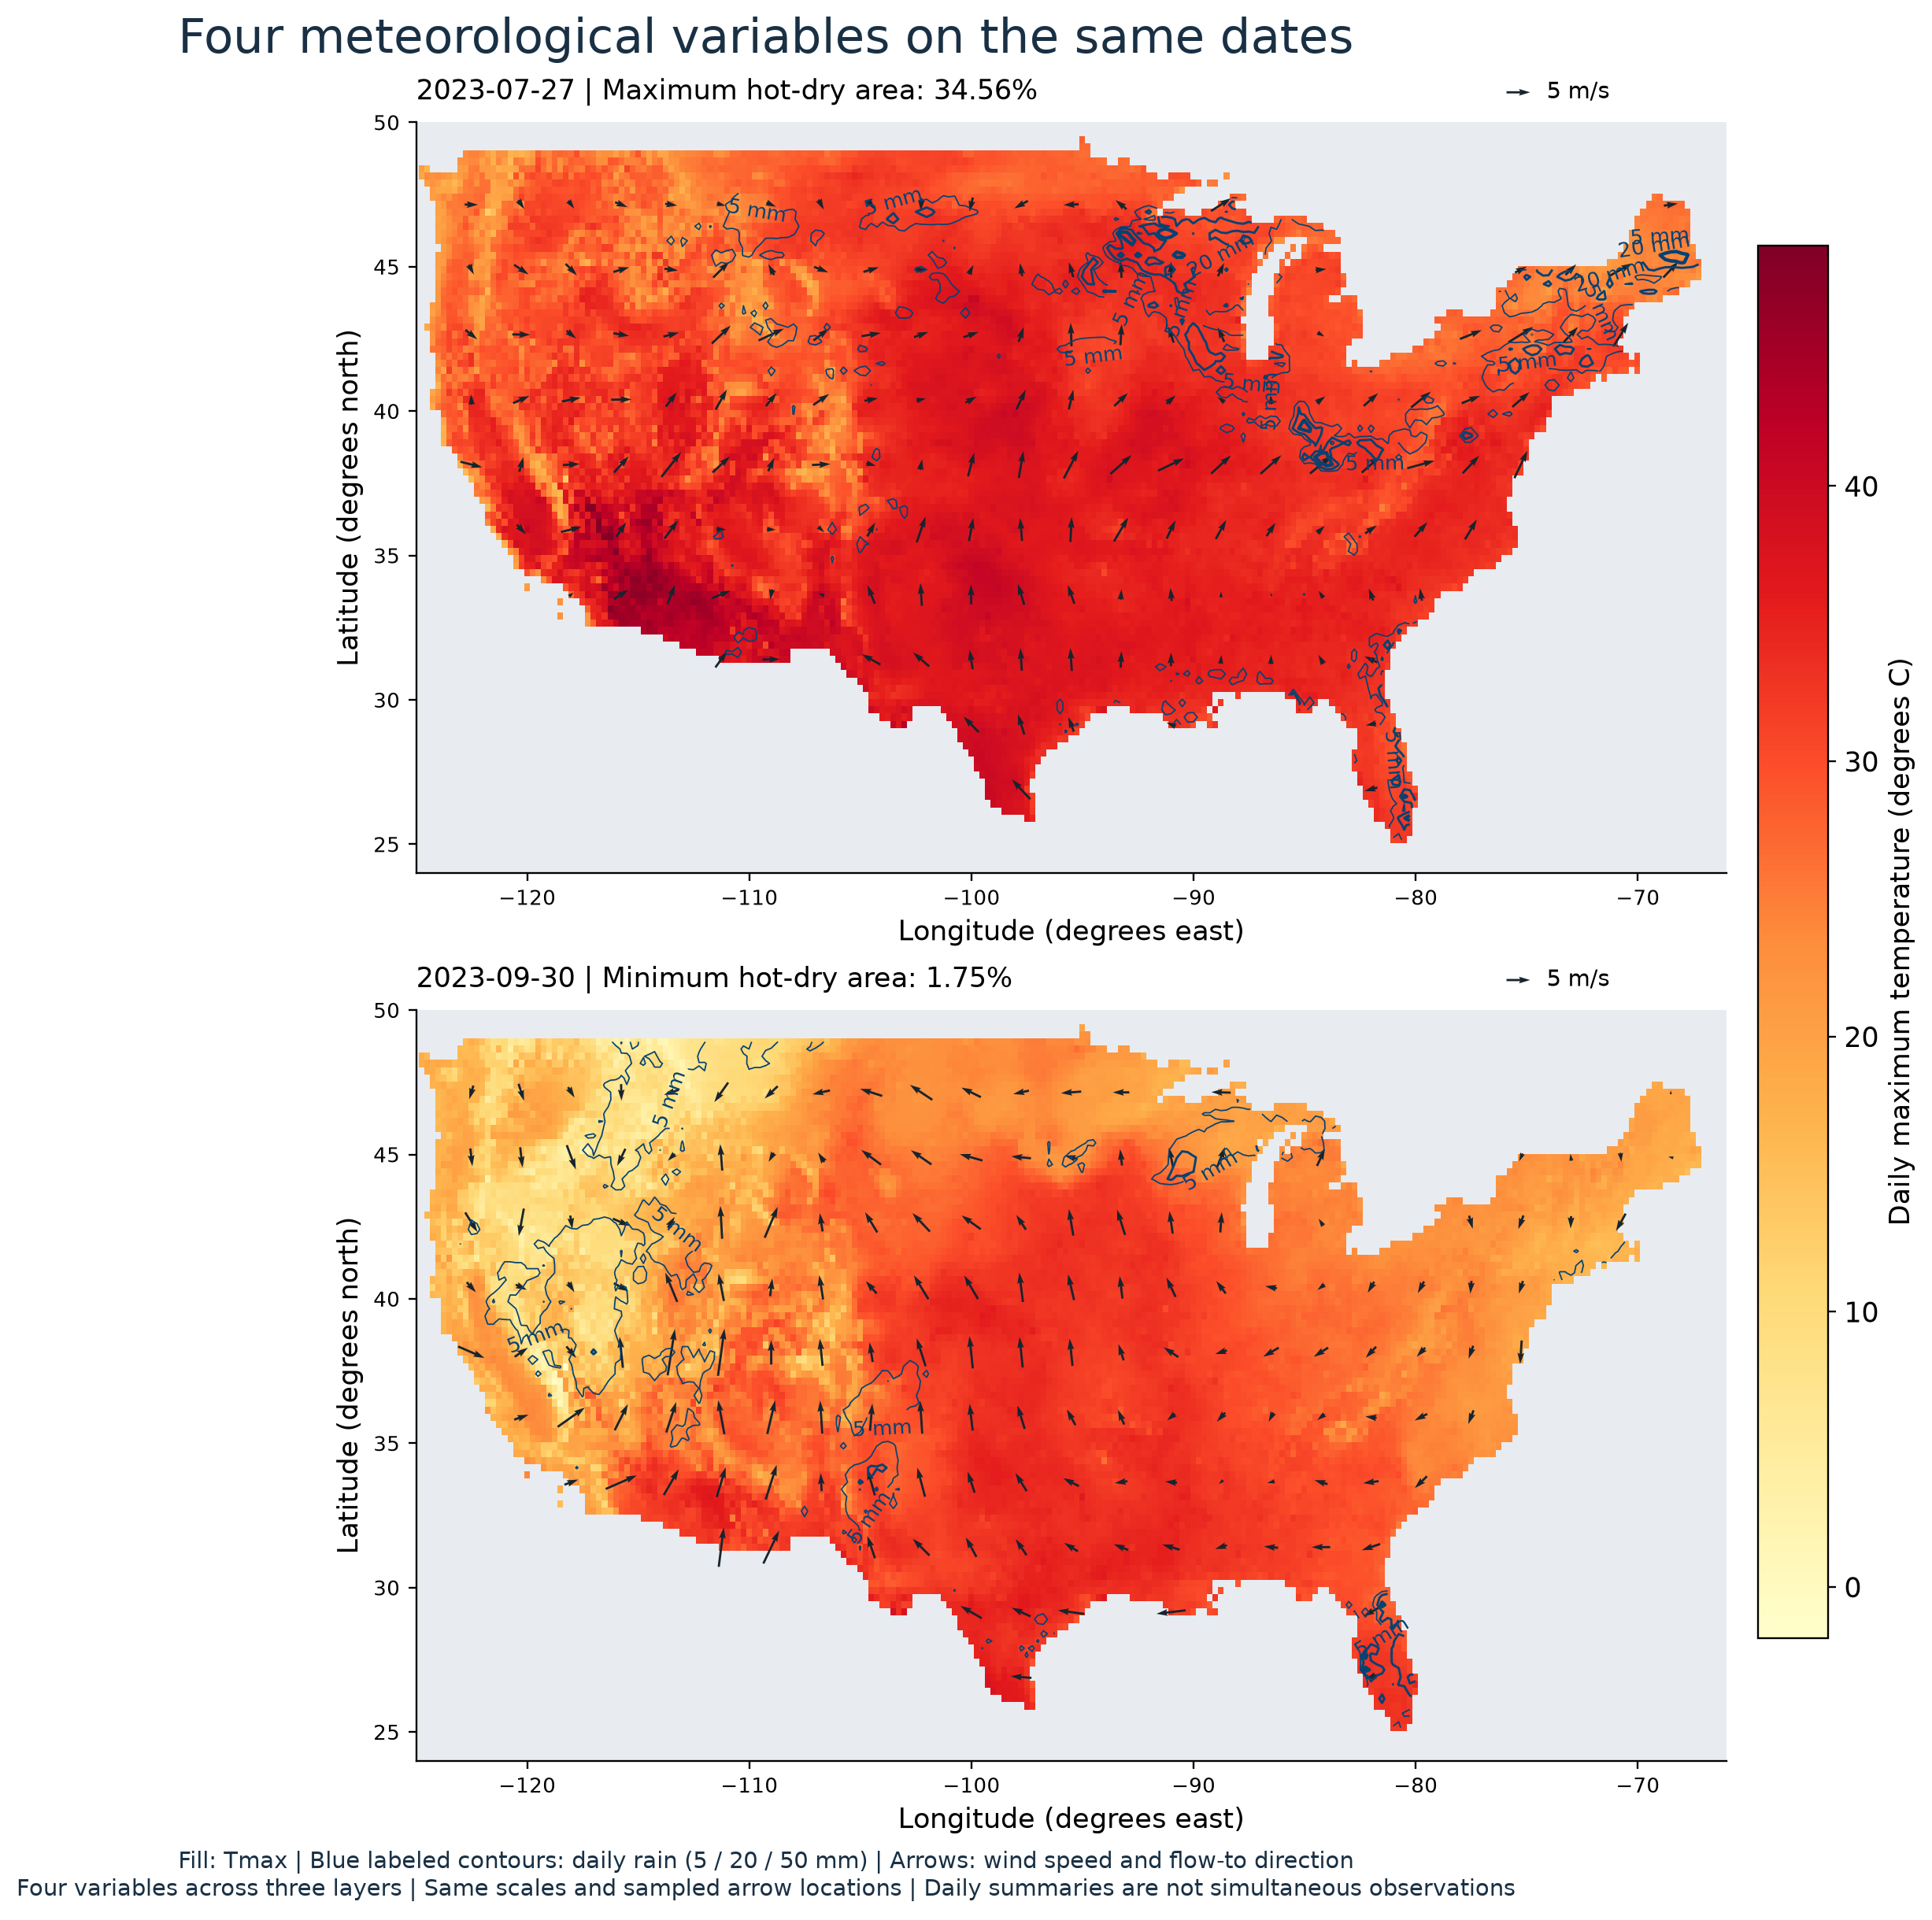
\includegraphics[width=\textwidth,height=0.59\textheight,keepaspectratio]{Fig28.png}

\caption{Aligned fields reveal spatial coincidence on two selected dates. {\footnotesize \href{https://aithal007.github.io/DV_assignment2/figures.html\#fig28}{\textcolor{accent}{\underline{View figure and interpretation online}}}}}\label{fig:28}

\end{figure*}

\noindent\textit{How to read the graph.} Two objectively selected dates share temperature colors, rain thresholds, arrow positions and speed keys. Layers reveal spatial coincidence on each date.

\paragraph{Question.} Can separate weather summaries hide where conditions occur together?



\paragraph{Visual encoding.} Both maps combine temperature color, rain contours and wind arrows. They show July 27 and September 30 on shared scales so the fields can be read at the same locations.



\paragraph{Why this visualization.} Separate temperature, rainfall and wind maps make it hard to check whether conditions occur at the same locations. The overlay aligns the three fields on one map. Two contrasting dates show what that alignment adds, while common visual scales keep the comparison meaningful.



\paragraph{Interpretation.} The objectively selected dates contrast hot-dry area coverage of 34.56\% on July 27 and 1.75\% on September 30. Common temperature colors, 5/20/50 mm rain contours and the same arrow positions permit spatial comparison. The overlay reveals where the fields coincide; three separate area means would not establish that.

The dates are deliberately contrasting examples, so they do not show how frequent either state is. The next full-period calculation evaluates all cells and dates. Moreover, daily maximum temperature, accumulated rain and daily wind summaries need not occur at the same hour: the overlay establishes cell-day alignment, not instantaneous physical simultaneity. This qualification preserves the spatial inference without turning co-location into an explanation of a weather mechanism.



\paragraph{Scope and reading note.} The dates were selected for this contrast. Co-location in a daily map does not prove a causal link or hourly coincidence.



\takeaway{Separate field summaries cannot establish that conditions coincide at the same place. The overlay aligns heat, rain and wind to reveal spatial coincidence on selected dates. Those examples motivate the complete-period overlap calculation rather than establish its frequency.

}

\noindent\textit{Analytical recommendation.} Inspect aligned fields before computing complete-period overlap.

\subsection{Fig. 29: Separate frequencies and shared occurrence}

\begin{figure*}[!tb]\centering

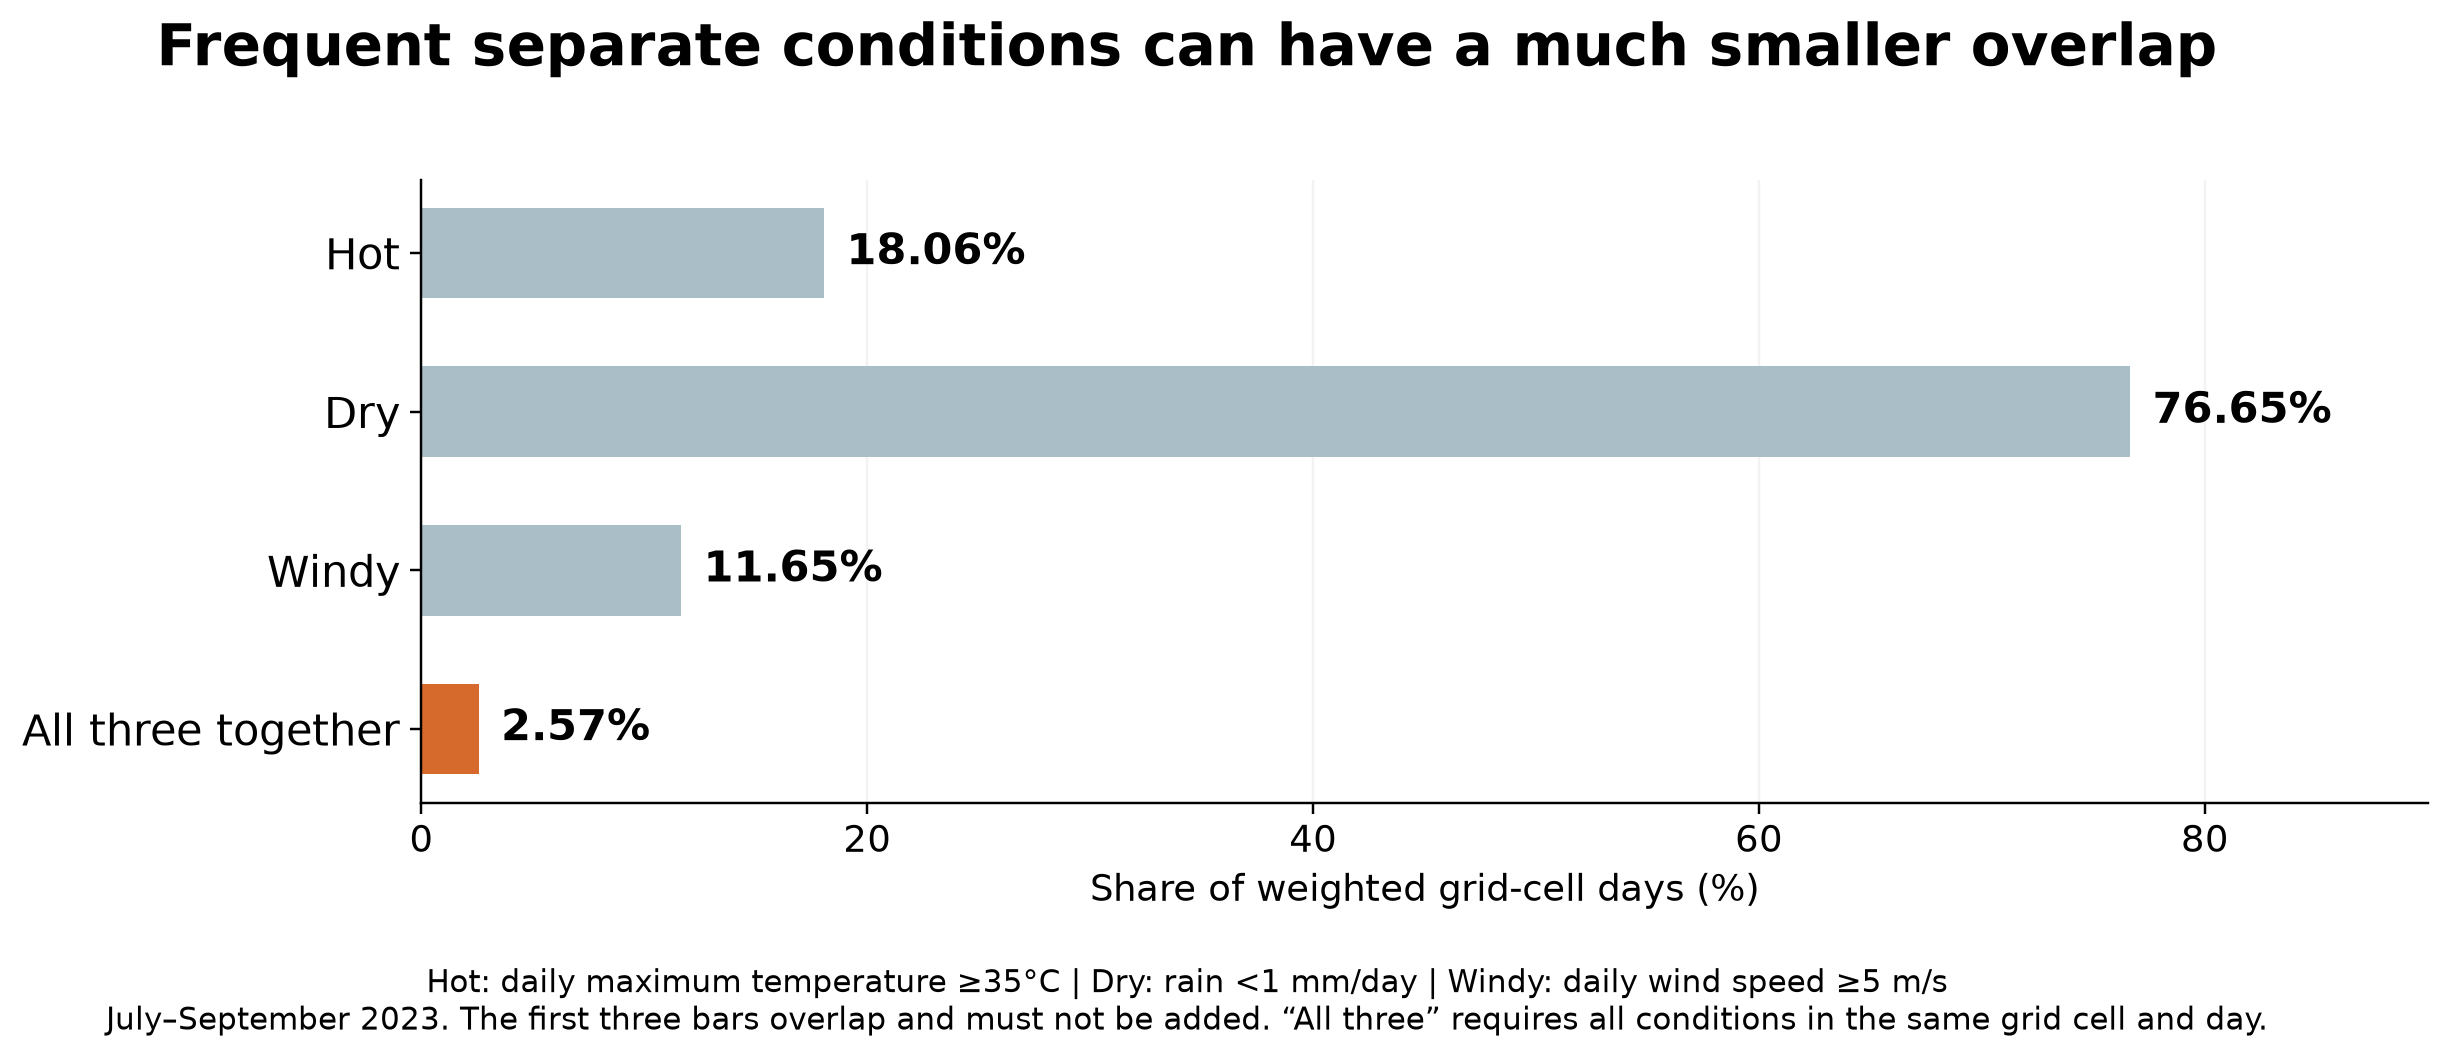
\includegraphics[width=\textwidth,height=0.21\textheight,keepaspectratio]{Fig29.png}

\caption{Frequent separate conditions have only 2.57\% joint occurrence. {\footnotesize \href{https://aithal007.github.io/DV_assignment2/figures.html\#fig29}{\textcolor{accent}{\underline{View figure and interpretation online}}}}}\label{fig:29}

\end{figure*}

\noindent\textit{How to read the graph.} Bars are weighted cell-day frequencies. The first three overlap; the fourth counts their exact intersection at the same cell and date.

\paragraph{Question.} How often do hot, dry and windy conditions occur together?



\paragraph{Visual encoding.} The first three bars count hot, dry and windy grid-cell days separately. The orange bar requires all three conditions in the same grid cell on the same day. All bars use the same weighted percentage scale.



\paragraph{Why this visualization.} With three conditions and a question about their joint occurrence, four bars give a direct answer. The first three establish how common each condition is; the fourth requires all three together. An intersection matrix would add symbols and combinations that are unnecessary for this comparison.



\paragraph{Interpretation.} Thresholds: hot means daily maximum temperature $\geq 35\,^{\circ}$C, dry means daily rain $< 1\,\text{mm/day}$, and windy means 10 m wind speed $\geq 5\,\text{m/s}$. The separate bars give about 18.06\% hot, 76.65\% dry and 11.65\% windy weighted cell-days. Their intersection is 2.57\%, calculated only when all three flags are true at the same cell and date. A very common dry condition therefore does not make the three-condition event equally common.

The bars overlap and must not be added. Multiplying the three marginal percentages would give about 1.61\% under an independence assumption, rather than the measured 2.57\%; separate frequencies do not recover the joint distribution. This answers the coincidence part of the main question with an explicit joint calculation. It is not a significance test, causal attribution or official hazard index, and neighboring cells/days are not independent samples.



\paragraph{Scope and reading note.} The first three bars overlap and must not be added. These percentages describe weighted grid-cell days, not people.



\takeaway{Common individual conditions need not produce common joint events. Although dry days occupy 76.65\% of weighted cell-days, only 2.57\% meet all three conditions together. Compute overlap at the same cell and date; separate marginal percentages cannot recover it.

}

\noindent\textit{Analytical recommendation.} Calculate joint conditions explicitly rather than multiplying marginal frequencies.

\subsection{Fig. 30: How often conditions occur and how long they last}

\begin{figure*}[!tb]\centering

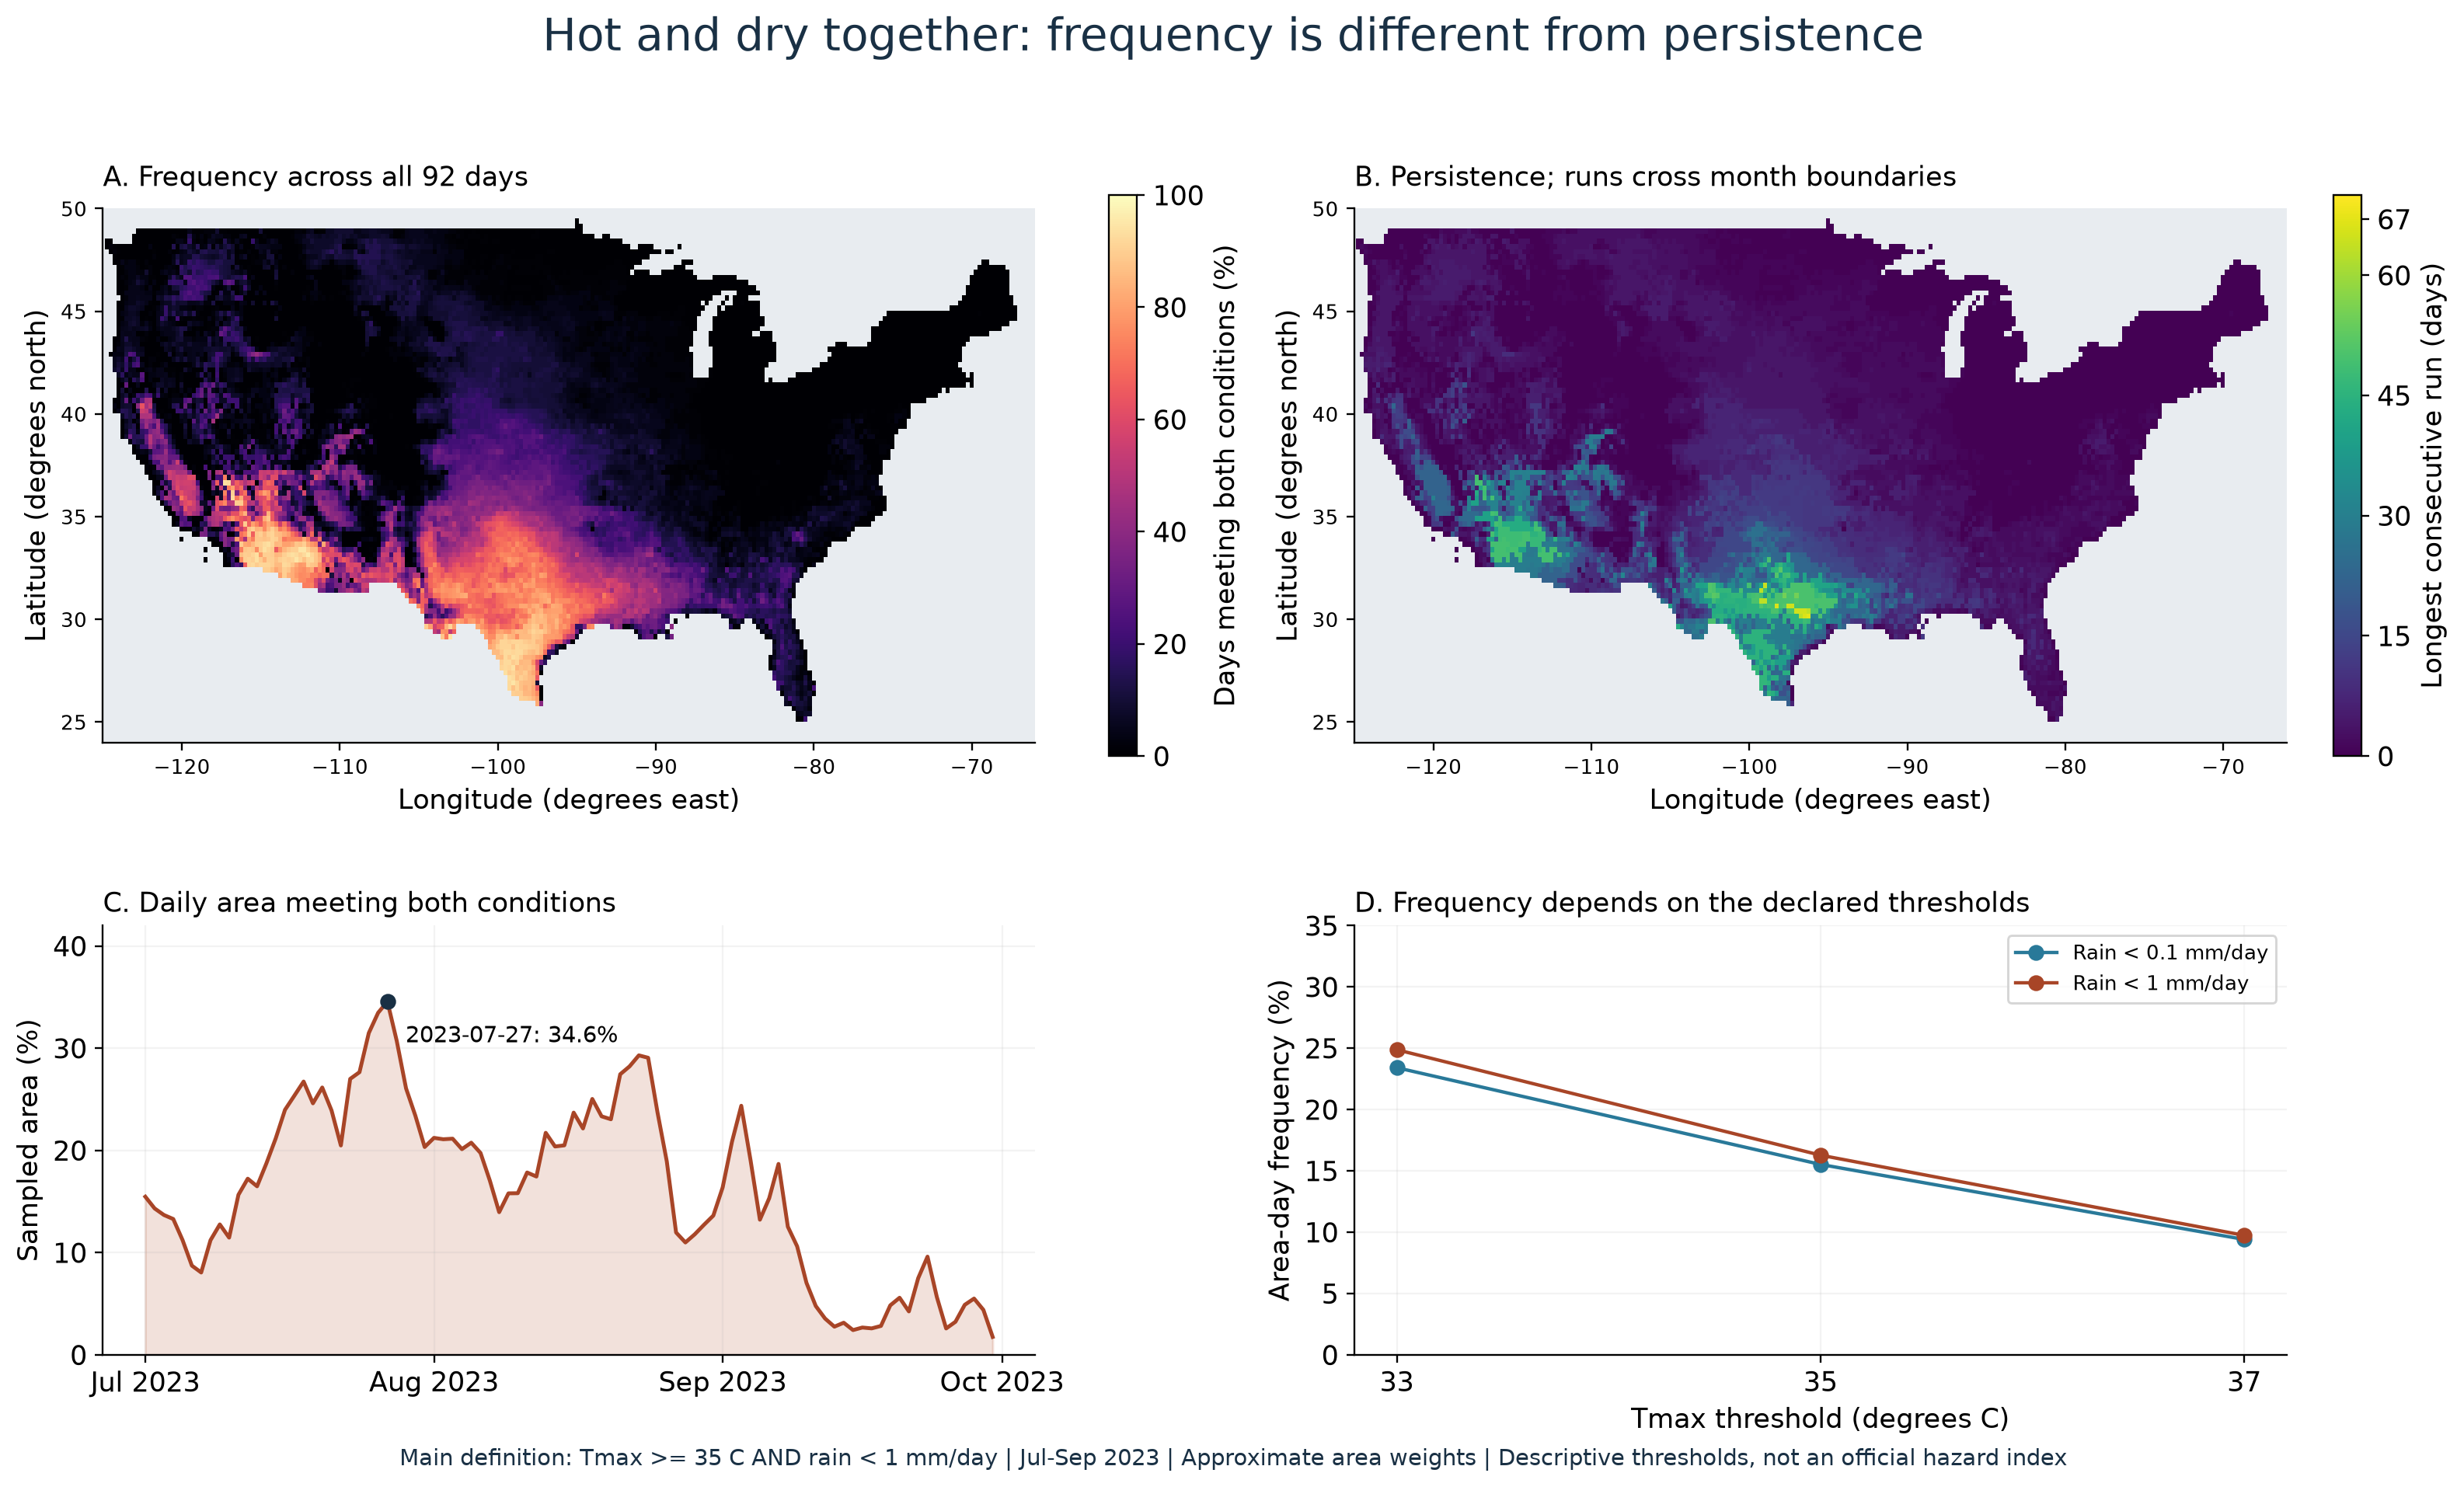
\includegraphics[width=\textwidth,height=0.42\textheight,keepaspectratio]{Fig30.png}

\caption{Frequency, uninterrupted duration and daily affected area describe different event properties. {\footnotesize \href{https://aithal007.github.io/DV_assignment2/figures.html\#fig30}{\textcolor{accent}{\underline{View figure and interpretation online}}}}}\label{fig:30}

\end{figure*}

\noindent\textit{How to read the graph.} Maps show frequency and longest run; the timeline gives daily affected area. The threshold panel repeats the calculation under six definitions.

\paragraph{Question.} Does the event count describe uninterrupted duration?



\paragraph{Visual encoding.} The maps compare hot-dry day frequency and the longest hot-dry run at each cell. The daily curve shows area coverage. The final panel repeats the calculation under alternative thresholds.



\paragraph{Why this visualization.} The shared-condition bars count occurrences but do not show whether they form long uninterrupted spells. Frequency and longest-run maps separate these two ideas. The daily coverage curve restores timing, and the threshold panel checks how the numerical result changes when the event definition changes.



\paragraph{Interpretation.} Hot-dry conditions occupy 16.27\% of weighted grid-cell days, while the maximum local uninterrupted run reaches 67 days. These quantities have different denominators: one summarizes area and time together; the other records the longest sequence at one location. The daily coverage curve adds whether a local persistent pattern also affects a large fraction of the footprint at once.

The final panel repeats frequencies at 33, 35 and 37 C with rain cutoffs of 0.1 and 1 mm/day, showing definition sensitivity. Runs touching the first/last observation may continue outside the window. The daily calendar that follows supplies a direct explanation of the frequency-persistence distinction: equal counts can be arranged into very different spells. Report occurrence, duration, coverage and threshold together before characterizing the event pattern.



\paragraph{Scope and reading note.} A run may start before or end after the study window. These daily thresholds do not diagnose drought or a heatwave.



\takeaway{Occurrence, uninterrupted duration and affected area describe different event properties. The 16.27\% hot-dry frequency and 67-day local maximum cannot substitute for each other. Combine their maps, daily coverage and threshold sensitivity before characterizing the seasonal pattern.

}

\noindent\textit{Analytical recommendation.} Report frequency, duration and affected area as separate event properties.

\subsection{Fig. 31: Daily event order separates frequency from persistence}

\begin{figure*}[!tb]\centering

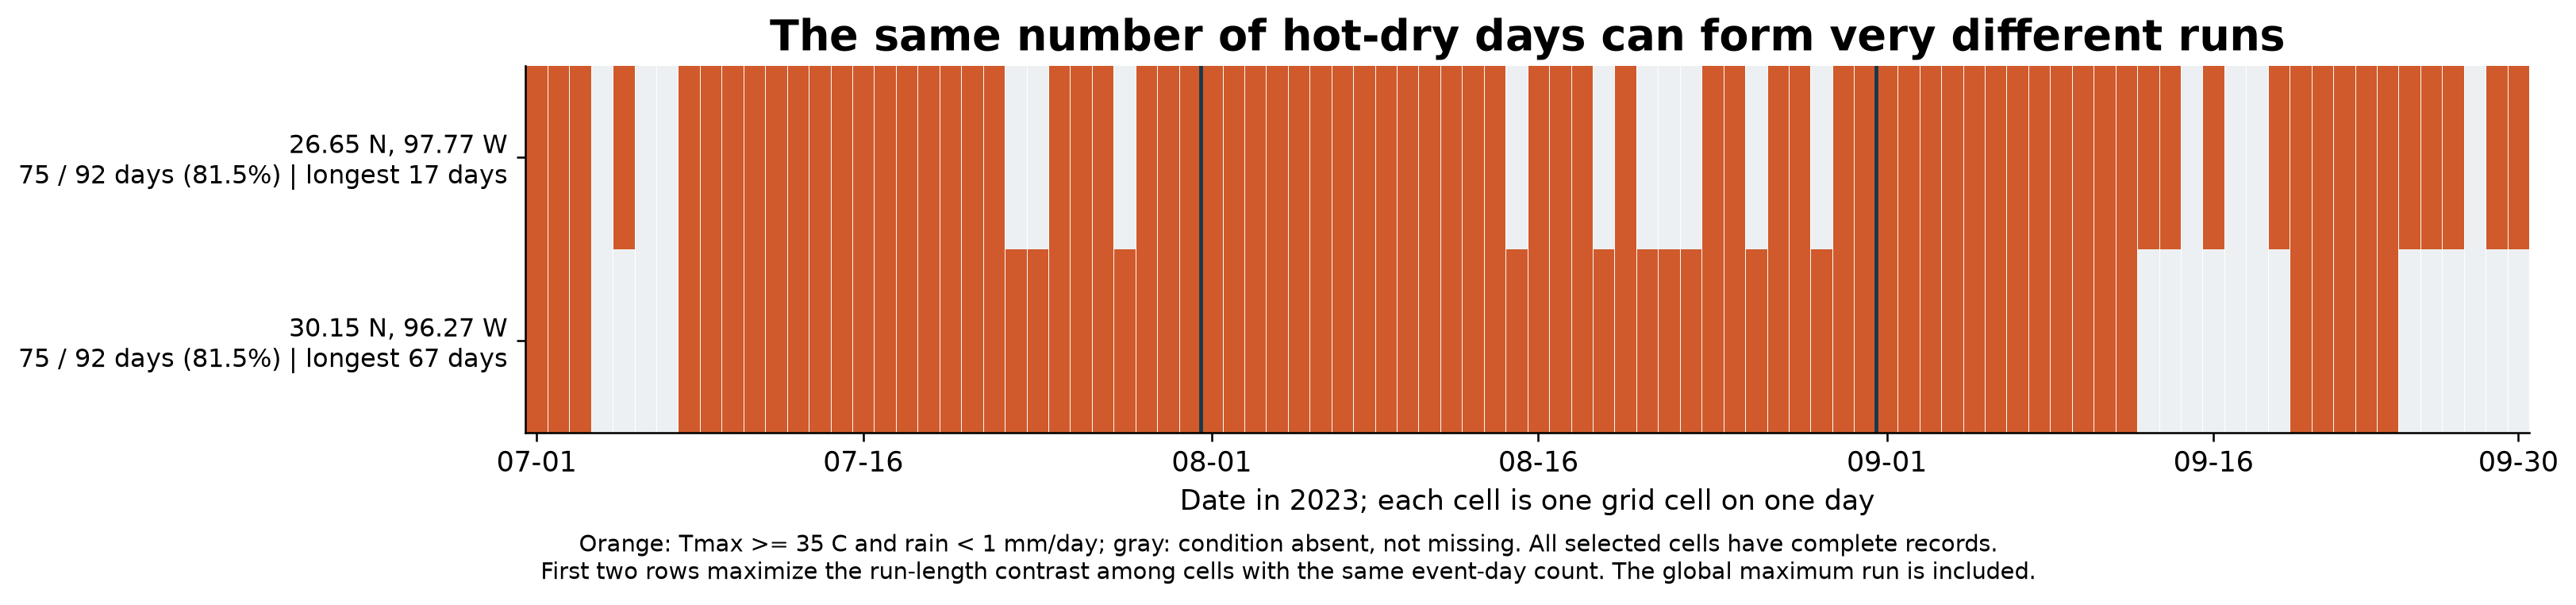
\includegraphics[width=\textwidth,height=0.18\textheight,keepaspectratio]{Fig31.png}

\caption{Equal 75-day counts conceal longest spells of 17 versus 67 days. {\footnotesize \href{https://aithal007.github.io/DV_assignment2/figures.html\#fig31}{\textcolor{accent}{\underline{View figure and interpretation online}}}}}\label{fig:31}

\end{figure*}

\noindent\textit{How to read the graph.} Rows are fixed grid cells, columns all 92 dates. Orange marks hot-dry days; gray marks absence. Row labels state counts and longest runs.

\paragraph{Question.} Can equal event frequencies hide different uninterrupted spells?



\paragraph{Visual encoding.} Rows are named grid cells; columns are all 92 days. Orange marks hot-dry conditions and gray their absence. Row labels give event-day counts and longest runs; vertical lines separate months.



\paragraph{Why this visualization.} Maps show where frequency and persistence occur. The calendar reveals the daily ordering that creates their difference.



\paragraph{Interpretation.} Both selected cells have 75 qualifying days out of 92 (81.5\%), yet the orange sequences form longest runs of 17 and 67 days. The interrupted first row and long continuous block in the second supply the visual mechanism behind that difference. A count discards the ordering that determines persistence.

Selection searches the common 13,416-cell footprint for the largest run-length contrast among equal positive day counts, with a declared tie rule. These are deliberately diagnostic examples, not typical cells. The maximum 67-day run is included. Fixed coordinates and the complete daily series avoid changing locations or omitting non-event days between panels. Boundary-touching spells may extend beyond the study window. This is the temporal detail needed to interpret the preceding frequency and run-length maps.



\paragraph{Scope and reading note.} The first pair deliberately maximizes the contrast among equal-count cells; it is not a typical sample. Runs may extend beyond the observed dates.



\takeaway{Equal event counts can hide very different persistence. Two cells each have 75 hot-dry days, yet longest spells of 17 and 67 days. Preserving daily order is necessary to distinguish scattered occurrences from sustained conditions.

}

\noindent\textit{Analytical recommendation.} Preserve daily order when duration matters.

\FloatBarrier

\section{Discussion}

Country averages conceal profile differences (71 of 454 nearly equal-adoption pairs meet P95, a 3.1x enrichment over the 5\% baseline), different paired paths, and both the 47\% within-region and 53\% between-region portions of measured variation. Broadband association weakens from $r_s = 0.831$ ($p < 0.001$) for levels to $r_s = 0.054$ ($p = 0.48$) for gains, with ceiling and floor effects limiting snapshot interpretation. Fixed cohorts reveal an absolute median gap that peaked at 62.7 points in 2011 before compressing to 53.8 in 2020, a pattern consistent with S-curve diffusion. Fig.~\ref{fig:1}'s documented feature-sensitivity analysis shows that omitting one indicator yields edge Jaccard overlaps of 0.338-0.512 (omitting mobile: 0.338; broadband: 0.412; landlines: 0.485; internet use: 0.512); the grouping is therefore a stated four-indicator definition, not an immutable country taxonomy.

Weather comparisons recover different omitted details: endpoint signs disagree with monthly means over 18.26\% of area; monthly totals conceal concentrated rainfall; equal 75-day event counts produce 17- versus 67-day runs. Synoptic weather features reflect documented meteorological events, including the July Southwest heat dome \cite{ref9}, Tropical Storm Harold's rainfall \cite{ref16}, and Hurricane Lee's coastal impact \cite{ref17}. Separate field frequencies also fail to recover the 2.57\% joint occurrence. These findings answer the main question through profiles, matched change and daily order.



\textbf{Scope and limits.} Country aggregates support descriptive comparisons, not causal attribution. Complete-case cohorts exclude missing observations; counts, shares and subscription rates use different denominators. The 2020 country values are source-published international estimates during the pandemic year and may be revised or modelled by their producers. Weather results concern one three-month interval and a fixed subsampled footprint, with approximate area weights and dependent cells/days. Daily fields need not coincide hourly; runs may extend beyond the window. Event cutoffs are descriptive, and period departures are not climate normals. Stride six reduces processing volume and display overlap; no native-resolution equivalence or finer-stride sensitivity check is claimed, so small-scale rainfall extremes may differ.



\section{Code and supporting files}

The README supplies setup and staged reproduction commands. Source country extracts, weather caches/acquisition metadata, custom contour code/tests, numbered images and editable LaTeX are included. The local launcher opens the browser user interfaces; optional Playwright commands regenerate browser exports and complete captures.



\section*{Author Contributions and Task Allocation}
Task responsibilities are assigned below. Each student implemented at least one SciVis and one InfoVis task with no shared figure ownership.
\par\smallskip\noindent{\footnotesize\begin{tabularx}{\columnwidth}{@{}p{0.27\columnwidth}Y@{}}\toprule\textbf{Member} & \textbf{Responsibility}\\\midrule
Parikshith Aithal K V (BT2024249) & \textbf{InfoVis:} Network (3 layouts, interaction) and parallel coordinates (bundling, brushing, reordering); \textbf{SciVis:} scalar color mapping, global/local scales, rainfall concentration. Figs 1--7, 18--19, 22--23 \\
Sindhoor Ganapathi Hegde (BT2024014) & \textbf{InfoVis:} Horizon and ridgeline plot variations (two variants each); \textbf{SciVis:} custom Marching Squares contour tracing, filled-band contours, contour GIF; weather persistence and event timing. Figs 14--17, 20--21, 24--25, 30--31 \\
Varshith M Gowda (BT2024227) & \textbf{InfoVis:} Treemap zoom/hierarchy experiments; association and catch-up comparisons across measures, regions and cohorts; \textbf{SciVis:} quiver grid-sampling and arrow-length encoding with wind roses and multivariable context. Figs 8--13, 26--29 \\\bottomrule\end{tabularx}}\par\smallskip

\section{Conclusion}

Similar summaries conceal different profiles, paths and daily sequences. Country-level pairing, consistent encodings and explicit temporal order provide the evidence needed to interpret the averages.



\begin{thebibliography}{17}

\bibitem{ref1} J. T. Abatzoglou, "Development of gridded surface meteorological data for ecological applications and modelling," International Journal of Climatology, vol. 33, pp. 121-131, 2013. gridMET product and documentation. \href{https://www.climatologylab.org/gridmet.html}{Online source}.

\bibitem{ref2} Our World in Data, "Internet" and underlying ITU/World Bank indicator metadata. The report uses the preserved A1 extracts, not a newly downloaded release. \href{https://ourworldindata.org/internet}{Online source}.

\bibitem{ref3} A. A. Hagberg, D. A. Schult and P. J. Swart, "Exploring network structure, dynamics, and function using NetworkX," Proceedings of the 7th Python in Science Conference, pp. 11-15, 2008. \href{https://aric.hagberg.org/papers/hagberg-2008-exploring.pdf}{Online source}.

\bibitem{ref4} D3 contributors, "What is D3?" and hierarchy/treemap documentation. JavaScript library used for the browser visualizations. \href{https://d3js.org/what-is-d3}{Online source}.

\bibitem{ref5} M. Bastian, S. Heymann and M. Jacomy, "Gephi: An Open Source Software for Exploring and Manipulating Networks," ICWSM, 2009. Assignment-permitted alternative; not used in this implementation. \href{https://doi.org/10.1609/icwsm.v3i1.13937}{Online source}.

\bibitem{ref6} ContourPy contributors, "Algorithm description," serial marching-squares/sweep contour generation and interpolation documentation. \href{https://contourpy.readthedocs.io/en/stable/description.html}{Online source}.

\bibitem{ref7} Matplotlib contributors, "Choosing Colormaps in Matplotlib," sequential and diverging palette guidance. \href{https://matplotlib.org/stable/users/explain/colors/colormaps.html}{Online source}.

\bibitem{ref8} N. Henry, J.-D. Fekete and M. J. McGuffin, "NodeTrix: A Hybrid Visualization of Social Networks," IEEE TVCG, vol. 13, no. 6, pp. 1302-1309, 2007. \href{https://www.dgp.toronto.edu/~mjmcguff/research/nodetrix/nodetrix.pdf}{Online source}.

\bibitem{ref9} NOAA National Centers for Environmental Information, "Assessing the U.S. Climate in July 2023," 2023. Independent context for the Southwest heat episode in the selected year. \href{https://www.ncei.noaa.gov/news/national-climate-202307}{Online source}.

\bibitem{ref10} J. Heinrich et al., "Evaluation of a Bundling Technique for Parallel Coordinates," 2011. Inspiration for the explicit-group, axis-preserving browser curves. \href{https://arxiv.org/abs/1109.6073}{Online source}.

\bibitem{ref11} E. Hovmoller, "The Trough-and-Ridge diagram," Tellus, vol. 1, no. 2, pp. 62-66, 1949. \href{https://doi.org/10.3402/tellusa.v1i2.8498}{Online source}.

\bibitem{ref12} J. Heer, N. Kong and M. Agrawala, "Sizing the Horizon: The Effects of Chart Size and Layering on the Graphical Perception of Time Series Visualizations," CHI, 2009. \href{https://hci.stanford.edu/publications/2009/heer-horizon-chi09.pdf}{Online source}.

\bibitem{ref13} M. Bruls, K. Huizing and J. J. van Wijk, "Squarified Treemaps," Data Visualization 2000, pp. 33-42, 2000. \href{https://doi.org/10.1007/978-3-7091-6783-0_4}{Online source}.

\bibitem{ref14} W. E. Lorensen and H. E. Cline, "Marching Cubes: A High Resolution 3D Surface Construction Algorithm," Computer Graphics, vol. 21, no. 4, pp. 163-169, 1987. \href{https://doi.org/10.1145/37401.37422}{Online source}.

\bibitem{ref15} D. Borland and R. M. Taylor II, "Rainbow Color Map (Still) Considered Harmful," IEEE Computer Graphics and Applications, vol. 27, no. 2, pp. 14-17, 2007. \href{https://doi.org/10.1109/MCG.2007.46}{Online source}.

\bibitem{ref16} NOAA National Hurricane Center, "Tropical Storm Harold Tropical Cyclone Report," 2023. \href{https://www.nhc.noaa.gov/data/tcr/AL092023_Harold.pdf}{Online source}.

\bibitem{ref17} NOAA National Hurricane Center, "Hurricane Lee Tropical Cyclone Report," 2023. \href{https://www.nhc.noaa.gov/data/tcr/AL132023_Lee.pdf}{Online source}.

\end{thebibliography}

\end{document}